\documentclass[compress]{beamer}
\usepackage{ifthen,verbatim}

\newcommand{\isnote}{}
\xdefinecolor{lightyellow}{rgb}{1.,1.,0.25}
\xdefinecolor{darkblue}{rgb}{0.1,0.1,0.7}

%% Uncomment this to get annotations
%% \def\notes{\addtocounter{page}{-1}
%%            \renewcommand{\isnote}{*}
%% 	   \beamertemplateshadingbackground{lightyellow}{white}
%%            \begin{frame}
%%            \frametitle{Notes for the previous page (page \insertpagenumber)}
%%            \itemize}
%% \def\endnotes{\enditemize
%% 	      \end{frame}
%%               \beamertemplateshadingbackground{white}{white}
%%               \renewcommand{\isnote}{}}

%% Uncomment this to not get annotations
\def\notes{\comment}
\def\endnotes{\endcomment}

\setbeamertemplate{navigation symbols}{}
\setbeamertemplate{headline}{\mbox{ } \hfill
\begin{minipage}{5.5 cm}
\vspace{-0.75 cm} \small
\end{minipage} \hfill
\begin{minipage}{4.5 cm}
\vspace{-0.75 cm} \small
\begin{flushright}
\ifthenelse{\equal{\insertpagenumber}{1}}{}{Jim Pivarski \hspace{0.2 cm} \insertpagenumber\isnote/\pageref{numpages}}
\end{flushright}
\end{minipage}\mbox{\hspace{0.2 cm}}\includegraphics[height=1 cm]{../cmslogo} \hspace{0.1 cm} \includegraphics[height=1 cm]{../tamulogo} \hspace{0.01 cm} \vspace{-1.05 cm}}

\begin{document}

\begin{frame}
\vfill
\begin{center}
\textcolor{darkblue}{\Large Realistic CRAFT1 MC Scenario}

\vfill
\begin{columns}
\column{0.3\linewidth}
\begin{center}
\large
\textcolor{darkblue}{Jim Pivarski}
\end{center}
\end{columns}

\begin{columns}
\column{0.3\linewidth}
\begin{center}
\scriptsize
{\it Texas A\&M University}
\end{center}
\end{columns}

\vfill
February 24, 2009
\end{center}
\end{frame}

%% \begin{notes}
%% \item This is the annotated version of my talk.
%% \item If you want the version that I am presenting, download the one
%% labeled ``slides'' on Indico (or just ignore these yellow pages).
%% \item The annotated version is provided for extra detail and a written
%% record of comments that I intend to make orally.
%% \item Yellow notes refer to the content on the {\it previous} page.
%% \item All other slides are identical for the two versions.
%% \end{notes}

\small

\begin{frame}
\frametitle{Realistic CRAFT1 MC Scenario}
\begin{itemize}\setlength{\itemsep}{0.2 cm}
\item A snapshot of the current state of the muon geometry, for use in
  MC for CRAFT1 analyses, can be generated via a deterministic script
  (random number seed is specified)

\item To run the script, check out V02-08-10 \mbox{of Alignment/MuonAlignment\hspace{-1 cm}}
\begin{itemize}
\item {\tt \scriptsize Alignment/MuonAlignment/python/MCScenario\_CRAFT1\_22X.py}
\end{itemize}

\item To look at it on the web, go to
\begin{itemize}
\item {\tt \scriptsize http://cmssw.cvs.cern.ch/cgi-bin/cmssw.cgi/CMSSW/} {\tt \scriptsize Alignment/MuonAlignment/python/MCScenario\_CRAFT1\_22X.py?view=markup}
\end{itemize}

\item For a copy of the SQLite file (to upload to the database), see
\begin{itemize}
\item {\tt \scriptsize /afs/cern.ch/user/p/pivarski/public/} \\ \hspace{1 cm}{\tt \scriptsize MCScenario\_CRAFT1\_22X\_V02-08-10.db}
\item Only DTAlignmentRcd and CSCAlignmentRcd are meaningful (APEs should be zero, as they are in data)
\item SQLite file tag names are equal to the record names
\end{itemize}

\end{itemize}
%% \hspace{-0.83 cm} \textcolor{darkblue}{\Large Outline2}
\end{frame}

\begin{frame}
\frametitle{The basic idea for DTs}
\begin{itemize}
\item Many DT chambers were observed with globalMuons, but only the
  best-measured ones were aligned
\item The residuals plots give us a good idea of where the rest of
  them are, with 1--2~mm uncertainty because we haven't decided that
  we can trust the residuals plots at a finer scale yet
\item Randomly generate DT chamber positions using observed residuals
  as the mean and 1--2~mm as the sigma of the Gaussian
\begin{itemize}
\item 1~mm of the ``1--2~mm'' is correlated between chambers in the
  same sector (because they lie on the same track)
\item another 1~mm is uncorrelated (a two-level hierarchy)
\end{itemize}
\item Any gaps in the residuals plots are filled in with Gaussians as
  wide as the corrections (4.5~mm in local $x$, 2.3~mm in $y$, and
  \mbox{1.0~mrad in $\phi_z$)\hspace{-1 cm}}
\item Local $x$, $y$, and $\phi_z$ were best determined, local $z$
  inferred from typical slopes of residuals, and $\phi_x$, $\phi_y$
  estimated from $\vec{B}$-field plots
\end{itemize}
\end{frame}

\begin{frame}
\frametitle{The basic idea for CSCs}
\begin{itemize}
\item CSC positions were observed with photogrammetry, and these
  corrections haven't been used in data processing yet
\begin{itemize}
\item therefore, they are currently a known error \\ (on the chamber-relative-to-disk level)
\end{itemize}
\item Disk-bending corrections were derived from DCOPS, which have
  a 1.4~mm uncertainty \mbox{(in $\vec{B}=0$ data, with respect to photogrammetry)\hspace{-1 cm}}
\begin{itemize}
\item this is correlated among all the chambers in the same ring that
  were corrected in $z$ and $\phi_x$
\end{itemize}
\item Whole-disk positions have some uncertainty in CMS \mbox{global coordinates\hspace{-1 cm}}
\item Three-level hierarchy: disk $\to$ disk-bending $\to$ individual chambers
\begin{itemize}
\item actually four levels, including layer-by-layer misalignments,
  but these are very small
\end{itemize}
\item CSC Overlaps information used to determine scale of chamber-by-chamber
  $\phi_y$ misalignments and layer misalignments
\end{itemize}
\end{frame}

\begin{frame}
\frametitle{What's on slides 6--70}
\begin{itemize}\setlength{\itemsep}{0.5 cm}
\item More explicit justification for each parameter (pages 6--13)
\begin{itemize}
\item including plots and references to talks which present them
\end{itemize}

\item Plots of every constant (pages 14--70)
\begin{itemize}
\item you can see some of the correlation-trends
\item photogrammetry CSC distribution is not exactly Gaussian
\end{itemize}

\item This is the last slide in the basic overview
\end{itemize}
\label{numpages}
\end{frame}

%% \section*{First section}
%% \begin{frame}
%% \begin{center}
%% \Huge \textcolor{blue}{First section}
%% \end{center}
%% \end{frame}

\begin{frame}
\frametitle{DT local $x$ and $y$}
\framesubtitle{(these are global $r\phi$ and $z$, respectively)}
\begin{itemize}
\item After a globalMuon alignment, uncertainties are not correlated on the station or wheel level
\item But they are correlated roughly by sector, due to the fact that
  chambers in the same sectors largely share tracks
\item The ``1--2~mm'' uncertainty is thus divided as
\begin{itemize}
\item 1~mm independent chamber-by-chamber error
\item 1~mm correlation within each sector \mbox{(sector$\otimes$wheel pairs, actually)\hspace{-2 cm}}
\end{itemize}
\item This is much more than the reproducibility of the procedure
  (0.098~mm in $x$ and 0.186~mm in $y$), so we are conservatively
  assuming a 1--2~mm error in the technique
\item The above only applies to aligned chambers; the other two categories are
\begin{itemize}
\item unaligned due to low statistics, but obvious from the residuals
  plots$^*$ what the true misalignment is (to the nearest millimeter)
\item too few tracks on the chamber to even appear in the plots
\end{itemize}
\end{itemize}

$^*$``more information'' \mbox{\tt \scriptsize http://indico.cern.ch/conferenceDisplay.py?confId=51267\hspace{-2 cm}}
\end{frame}

\begin{frame}
\frametitle{DT local $x$ and $y$ (continued)}
\begin{itemize}
\item Therefore I looked at each chamber, wrote down the apparent
  misalignment, and used that as a mean for the \mbox{Gaussian-generated errors\hspace{-1 cm}}
\begin{itemize}
\item e.g.\ a chamber looks misaligned by 6~mm, and we trust the
  procedure to 1~mm, so we generate a random misalignment with mean
  6~mm and sigma 1~mm
\end{itemize}
\item The table of ``observed by hand'' misalignments are in the script
\item Chambers with too few tracks to appear in the plots were
  randomly generated with a mean of 0 and a sigma of \mbox{4.5~mm ($x$) and 2.3~mm ($y$)\hspace{-1 cm}}
\begin{center}
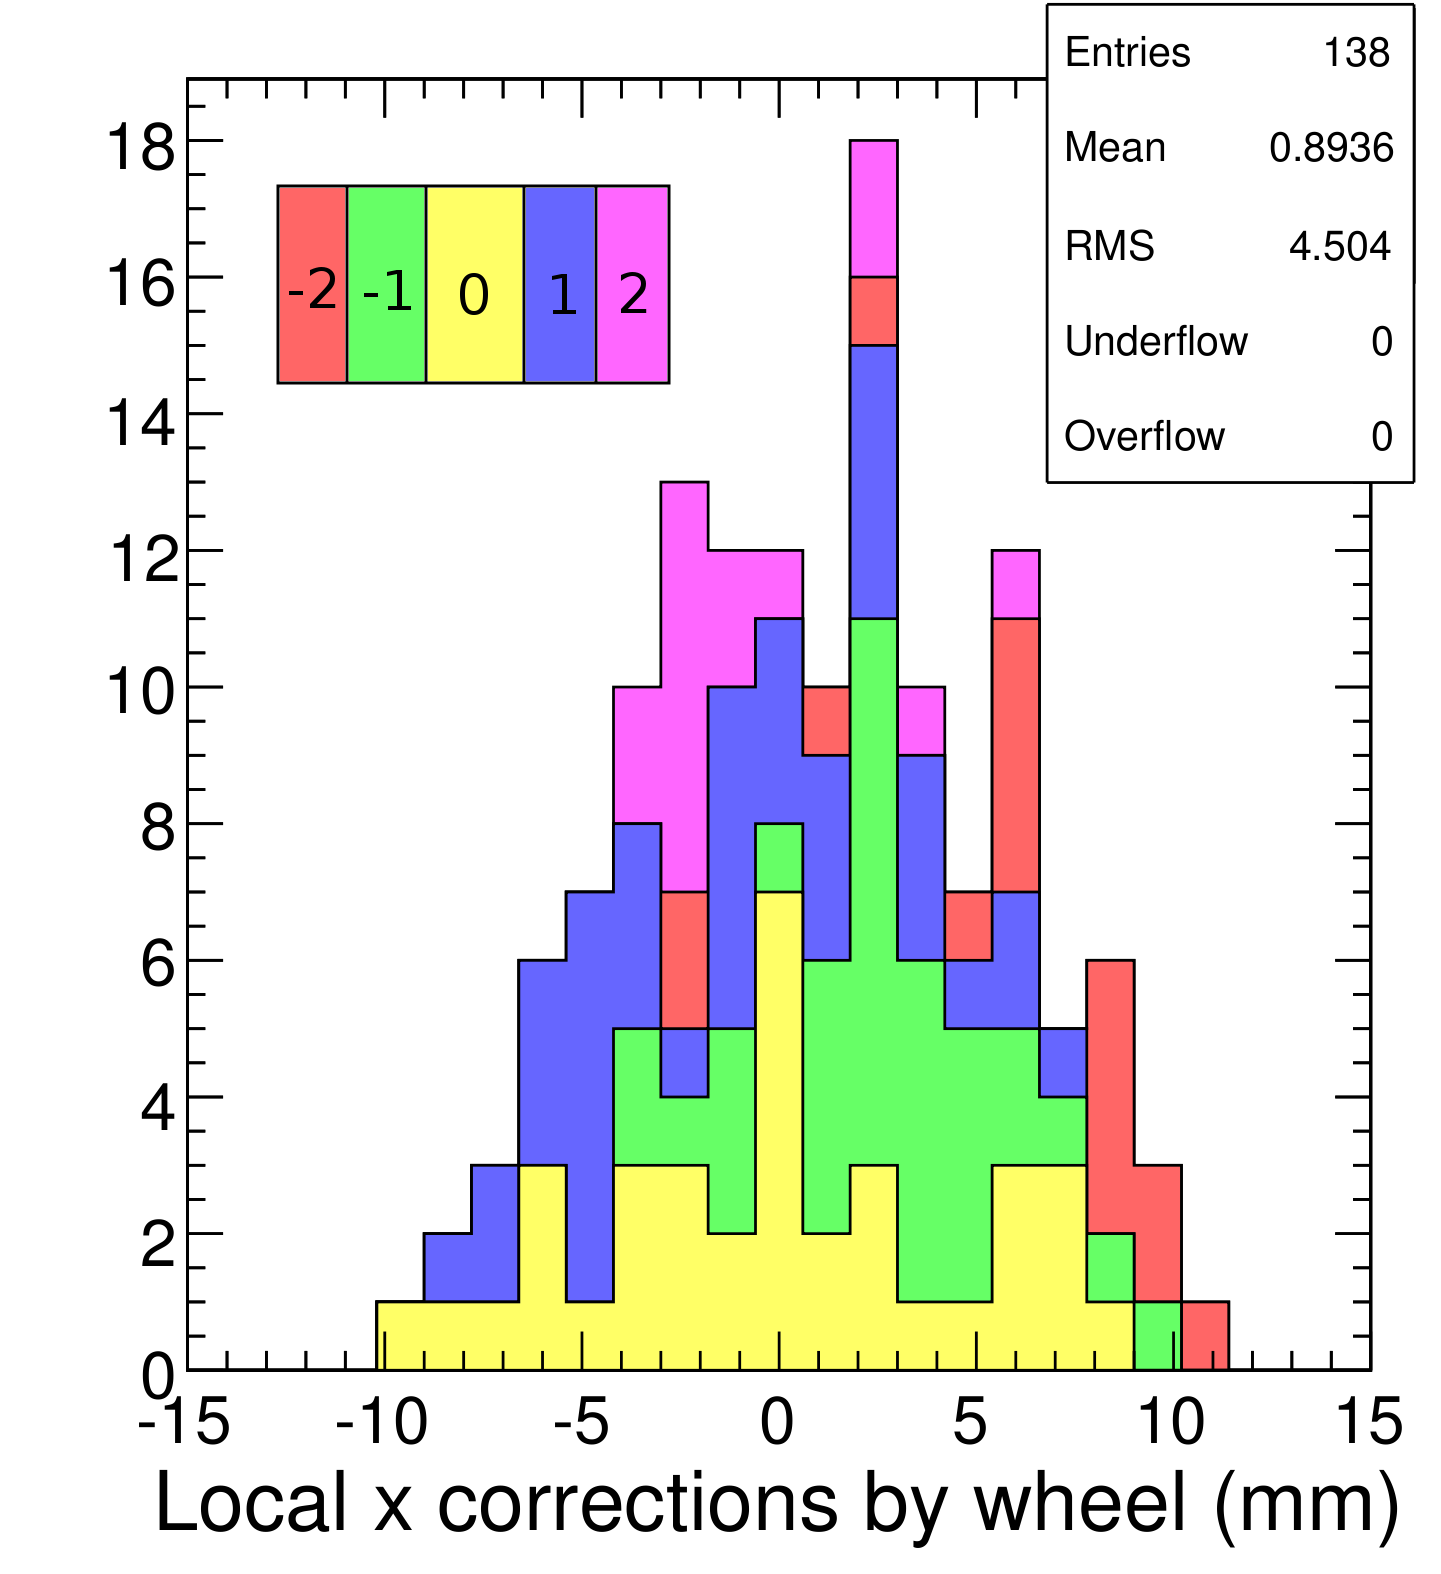
\includegraphics[width=0.3\linewidth]{report2_xbywheel.png} 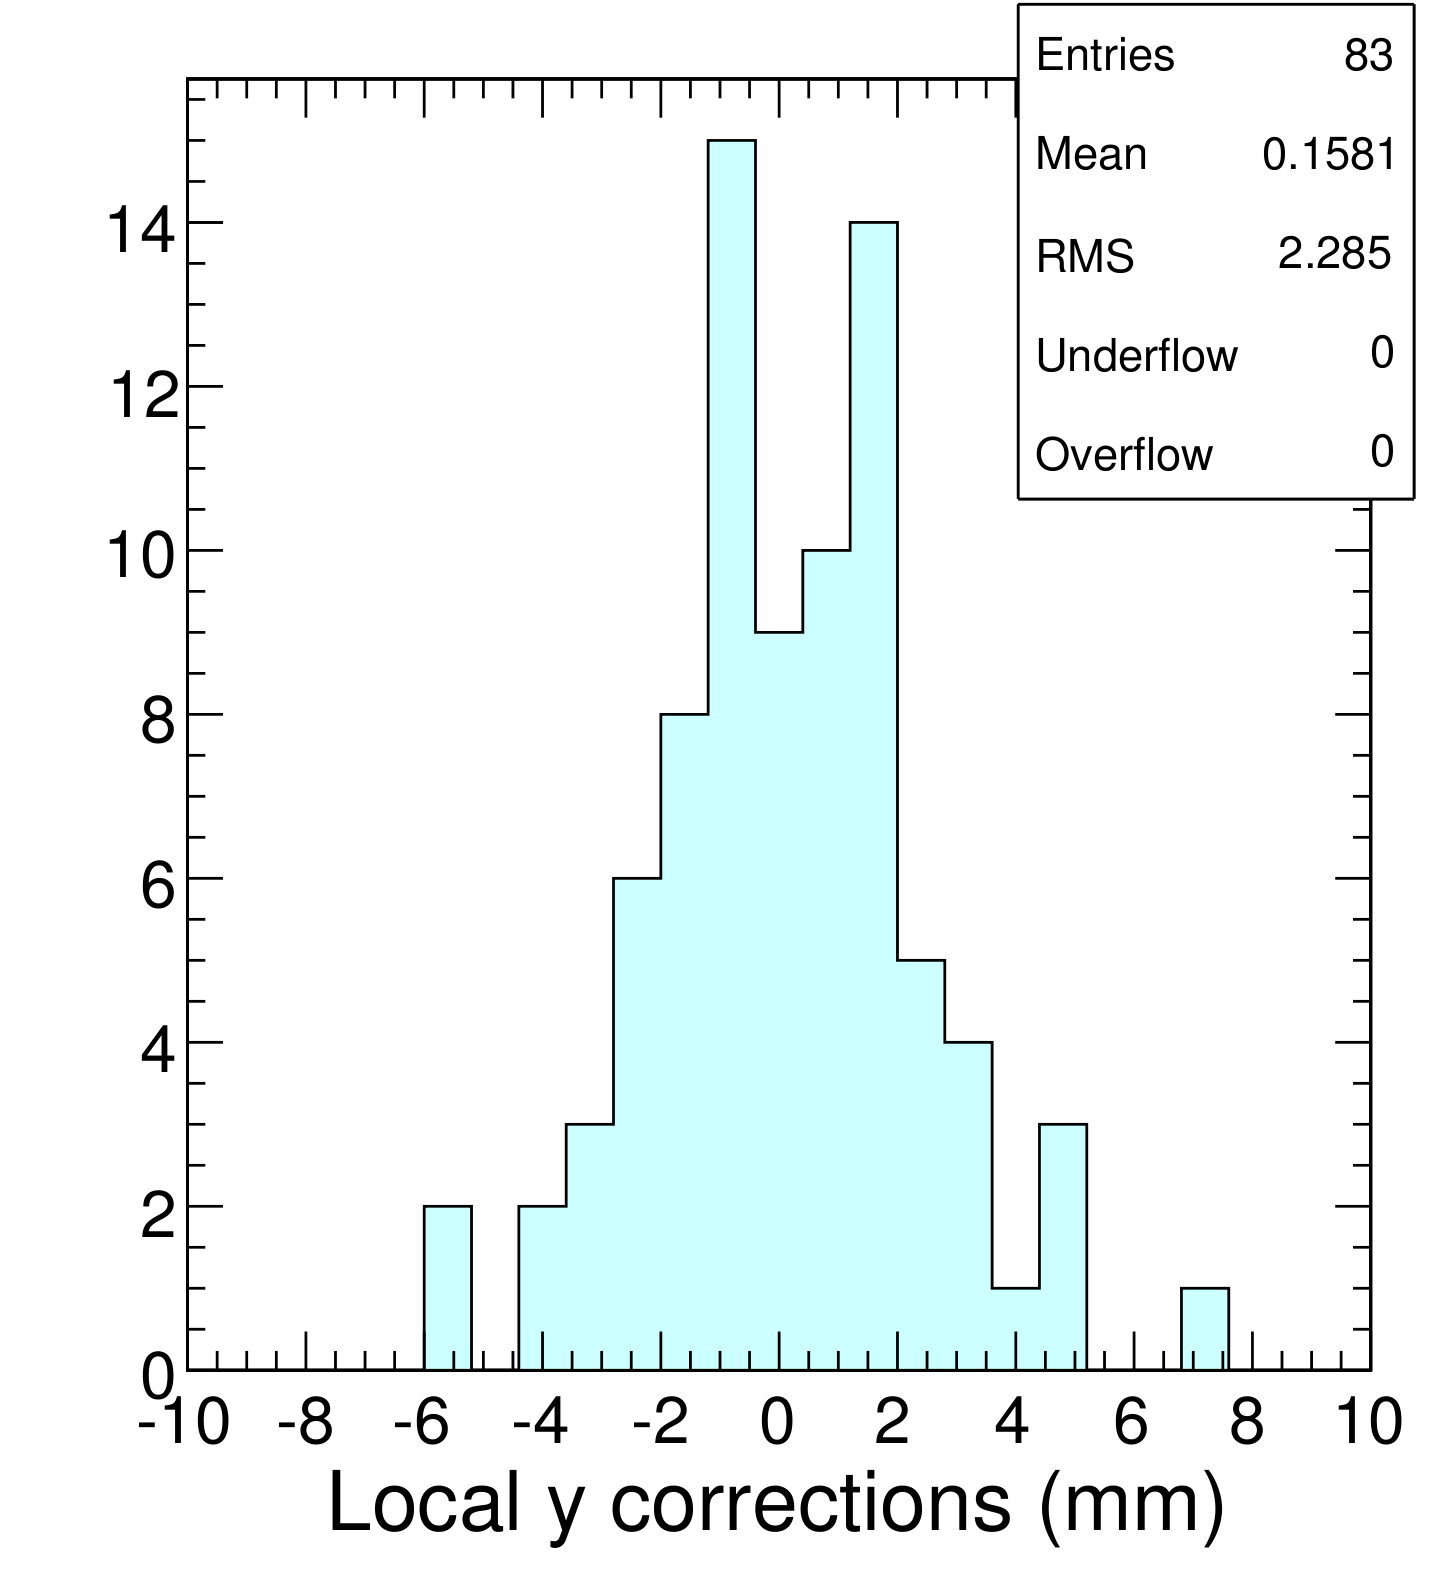
\includegraphics[width=0.3\linewidth]{report2_y.png}
\end{center}

\item The scenario will therefore have the right resolution($\phi$, $z$) \mbox{dependence\hspace{-1 cm}}
\end{itemize}
\end{frame}

\begin{frame}
\frametitle{DT local $\phi_z$}
\framesubtitle{(this is rotation in the layer's measurement plane)}
\begin{itemize}
\item Unlike the $x$ and $y$ translations, $\phi_z$ is a local
  measurement, depending only on the difference between nearby
  residuals
\item One can imagine biases which distort the track source with a
  ``low multipole'' dependence (e.g.\ $\sin\phi$, $\cos 2\phi$, $z$,
  $z^2$\ldots), but this has minimal impact on $\phi_z$
\item Therefore, take the $\phi_z$ misalignment for aligned chambers
  to be the reproducibility of the procedure (RMS of second-iteration
  corrections): 0.058~mrad
\item For unaligned chambers, it's 1.0~mrad, the typical correction \\ (plot label should be ``mrad'', not ``mm'')
\end{itemize}

\vspace{-0.8 cm}
\hfill 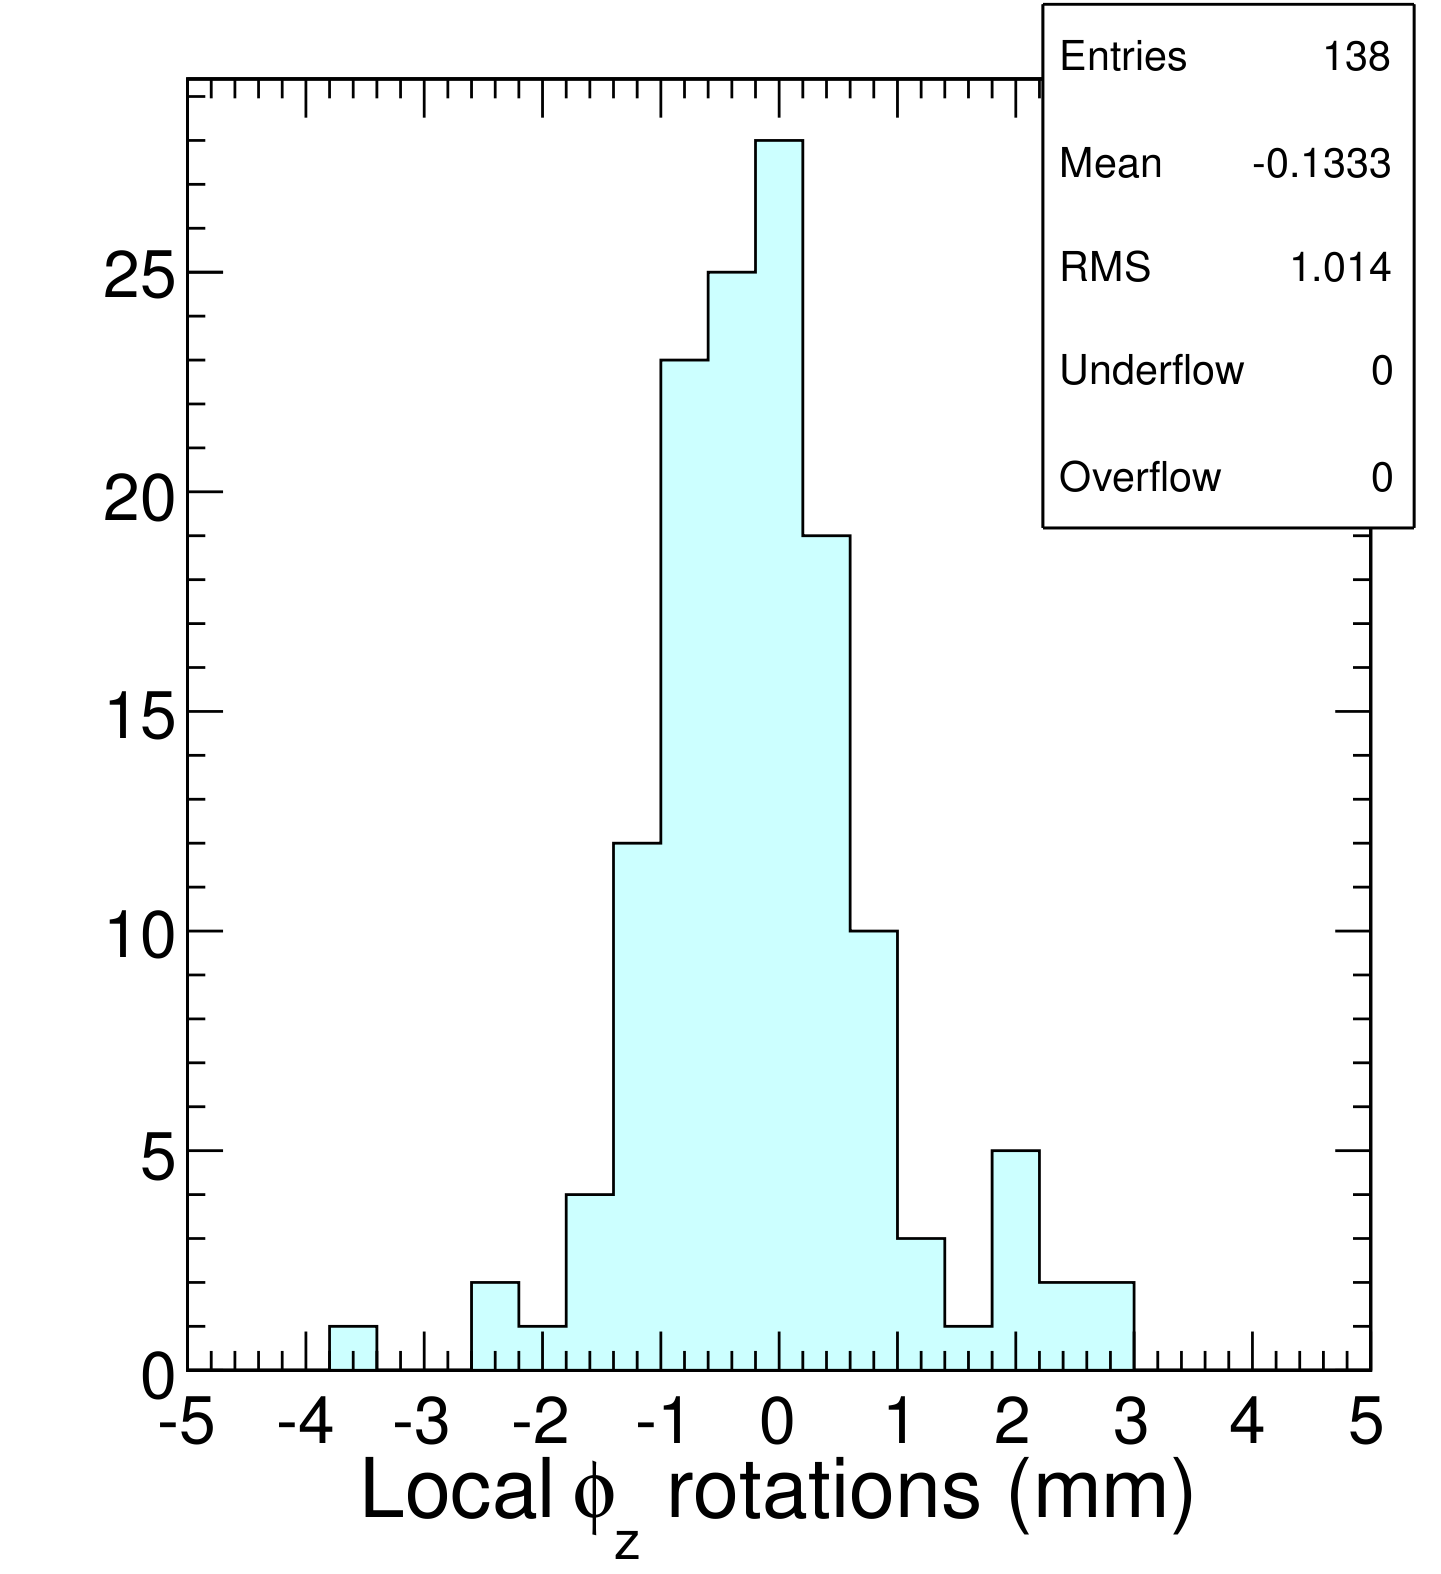
\includegraphics[width=0.3\linewidth]{report2_phiz.png}
\end{frame}

\begin{frame}
\frametitle{DT local $\phi_x$ and $\phi_y$}
\begin{itemize}
\item Magnetic field measurements compared track and segment angles, observed $\phi_y$ misalignments as a by-product of measuring field

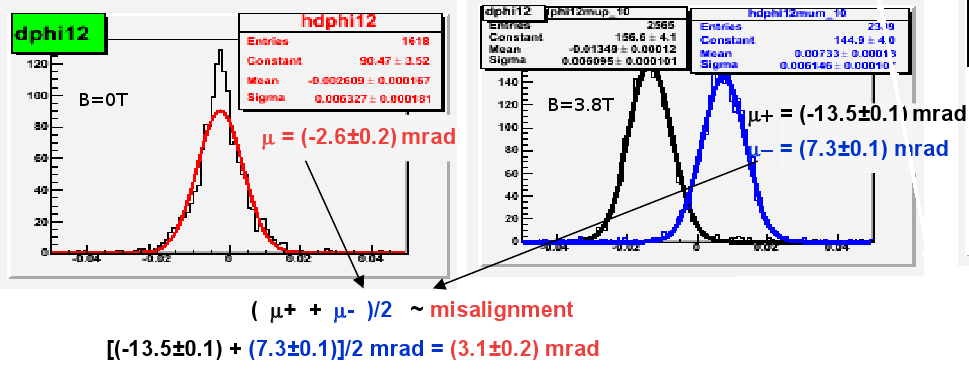
\includegraphics[width=\linewidth]{segment_phiy.png}

\item Conclude from slide 12 of Sara's talk at {\tt \scriptsize http://indico.cern.ch/conferenceDisplay.py?confId=51559} \\ that 3~mm $\phi_y$ angles are typical

\item Assume the same for $\phi_x$

\item Note: this comes from only one measurement!
\end{itemize}
\end{frame}

\begin{frame}
\frametitle{CSC hierarchy}
\begin{itemize}
\item CSCs have never been (robustly) measured by globalMuons, so uncertainties are still correlated via the following hierarchy:
\begin{itemize}\setlength{\itemsep}{0.2 cm}
\item CSC disks: aligned in the cavern with photogrammetry 
\item CSC rings (disk bulging): $z$ and chamber-$\phi_x$ corrections with DCOPS/SLMs (correlated within each ring)
\item CSC chambers: uncorrected translations/rotations known from photogrammetry data (except $\phi_y$, that comes from \mbox{CSC Overlaps)\hspace{-1 cm}}
\item CSC layers: observed tiny misalignments, put them in the scenario anyway
\end{itemize}
\end{itemize}

\vfill
\hspace{-0.83 cm} \textcolor{darkblue}{\Large CSC disk precision}

\begin{itemize}
\item 0.5~mm $x$-$y$ precision, 3~mm $z$, and 0.5~mrad in all three angles
\end{itemize}
\end{frame}

\begin{frame}
\frametitle{CSC ring precision}
\framesubtitle{($z$ and $\phi_x$ to represent disk bulging)}
\begin{itemize}
\item DCOPS/PG comparison in $z_{\mbox{\scriptsize CMS}}$:  page~7 of Samir's talk on {\tt \scriptsize http://indico.cern.ch/conferenceDisplay.py?confId=39027}

\begin{center}
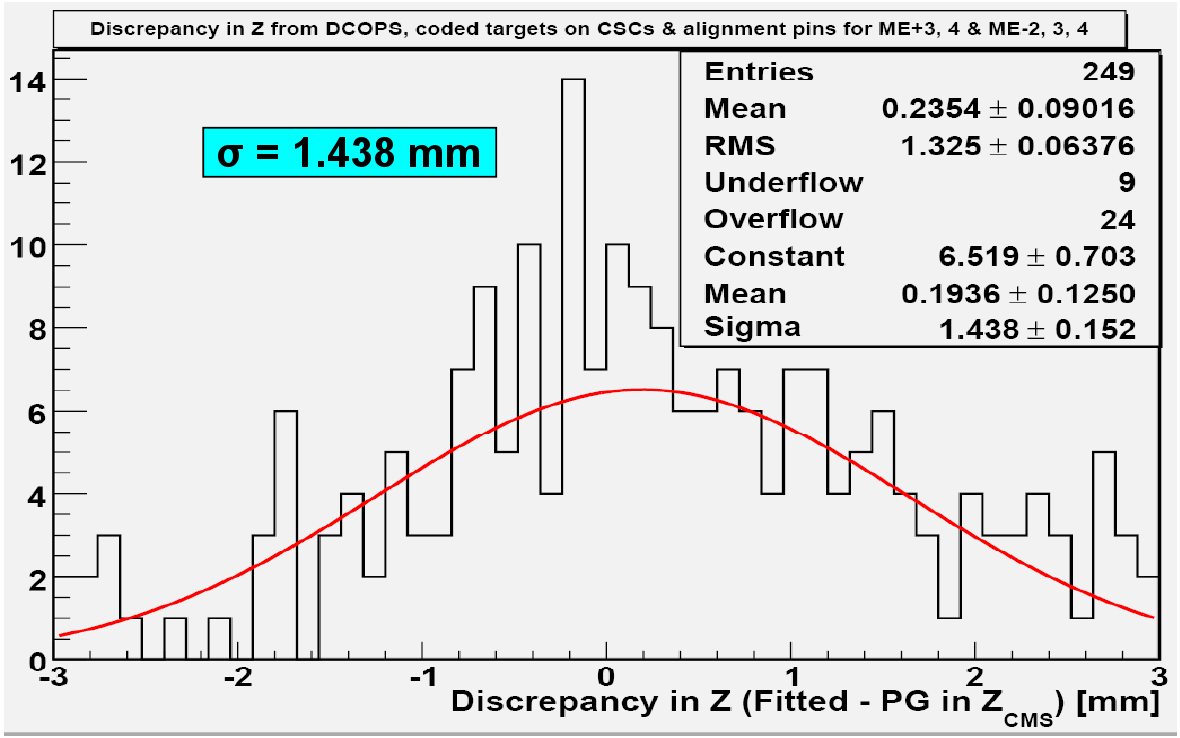
\includegraphics[width=0.8\linewidth]{dcops_in_z_replacement.png}
\end{center}

\item Implies $z$ uncertainty is 1.438~mm and $\phi_x$ uncertainty is 0.57~mrad
\end{itemize}
\end{frame}

\begin{frame}
\frametitle{CSC chamber misalignments}
\begin{itemize}
\item Karoly has converted all CSC photogrammetry into a
  CSCAlignmentRcd, so it should be considered for the next
  reprocessing (whenever that is)
\item In the meantime, these are known, uncorrected-for constants, which
  exactly quantifies our error \mbox{(up to any changes the $\vec{B}$-field might make)\hspace{-1 cm}}
\item When chambers have no photogrammetry information (ME1/1 and
  incomplete data in other rings), we use the RMS of the others:
\begin{itemize}
\item 1.2~mm in $x$, 1.0~mm in $y$, 1.2~mm in $z$, 1.1~mrad in $\phi_x$, 0.56~mrad in $\phi_z$
\end{itemize}
\end{itemize}

\begin{columns}
\column{0.6\linewidth}
\begin{itemize}
\item Two alignment pins cannot determine $\phi_y$; get an RMS of that from
  beam-halo CSC Overlaps measurement (left: measured, right: MC to gauge the precision)
\end{itemize}

\column{0.5\linewidth}
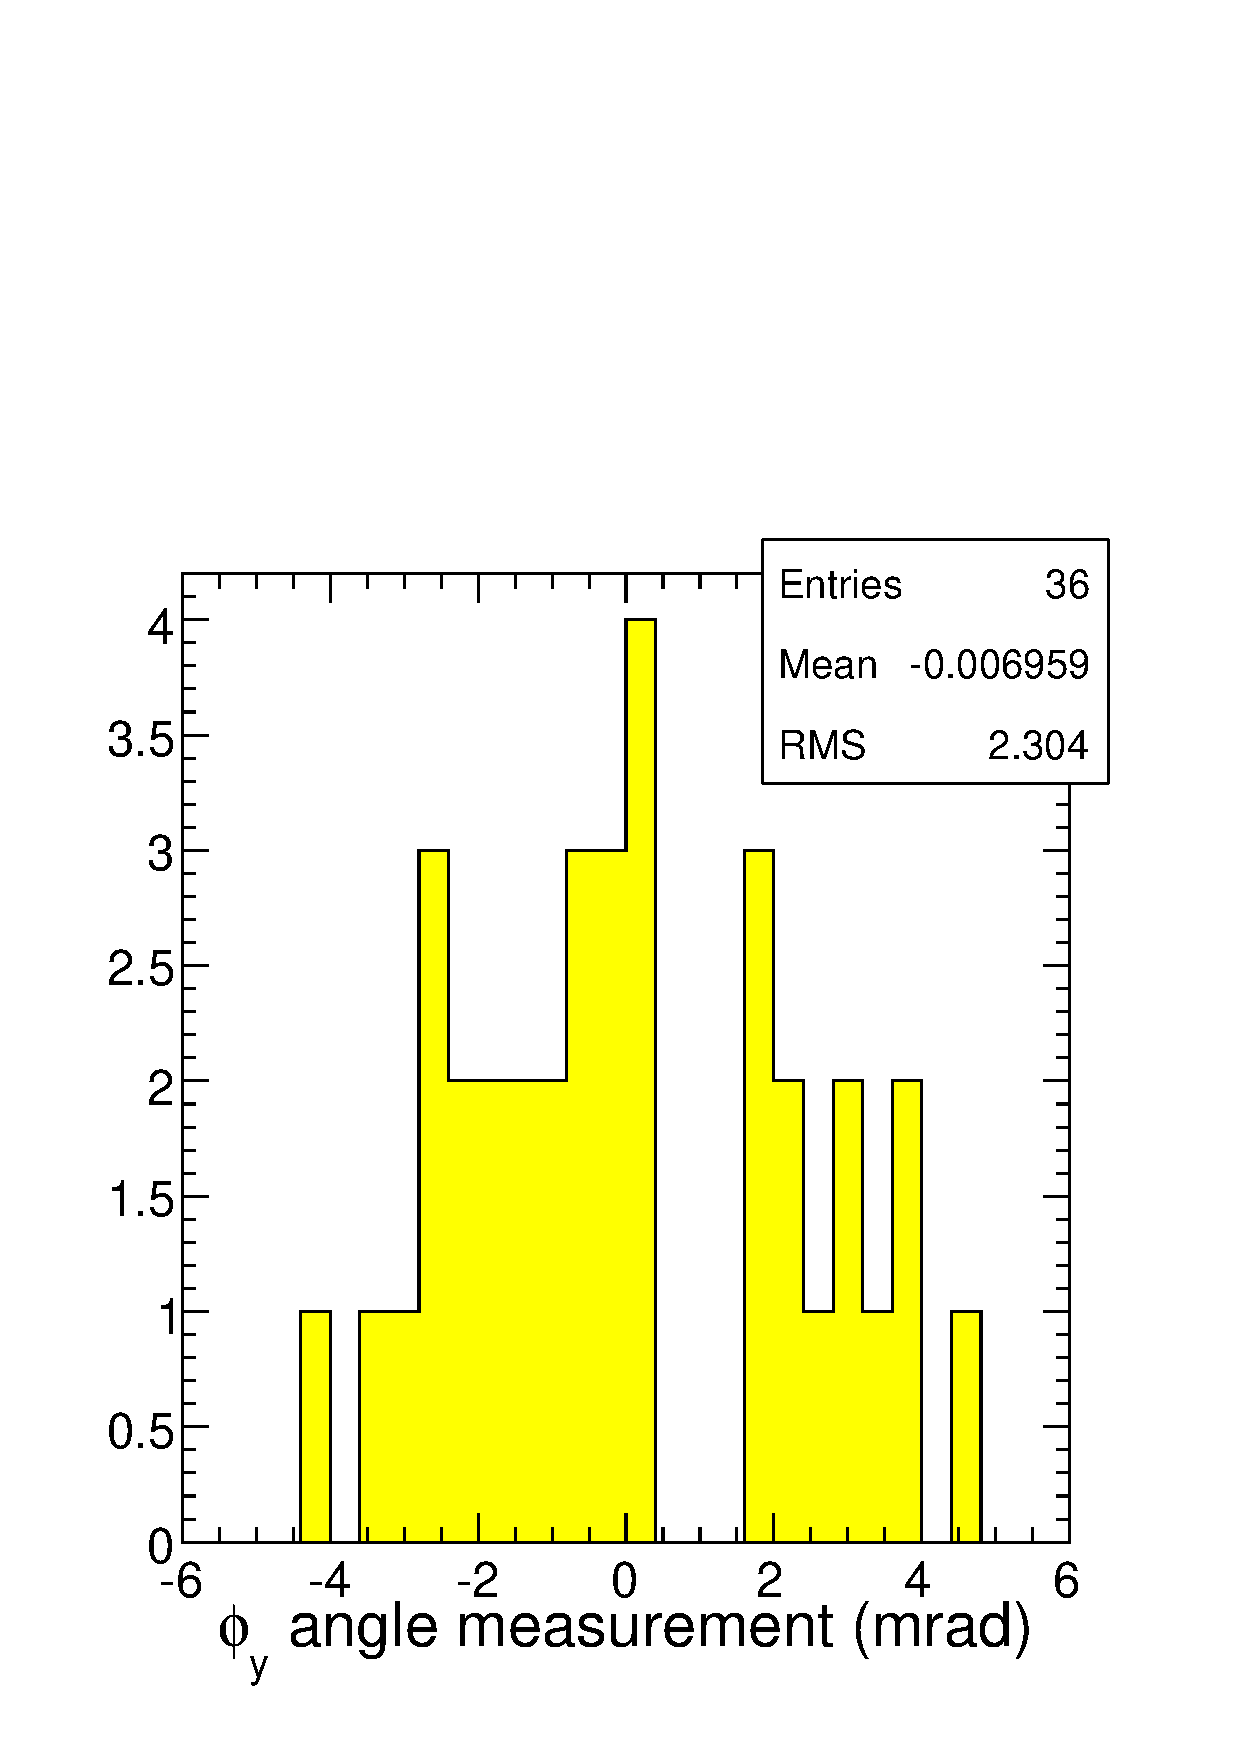
\includegraphics[width=0.5\linewidth]{measured_phiy.pdf} 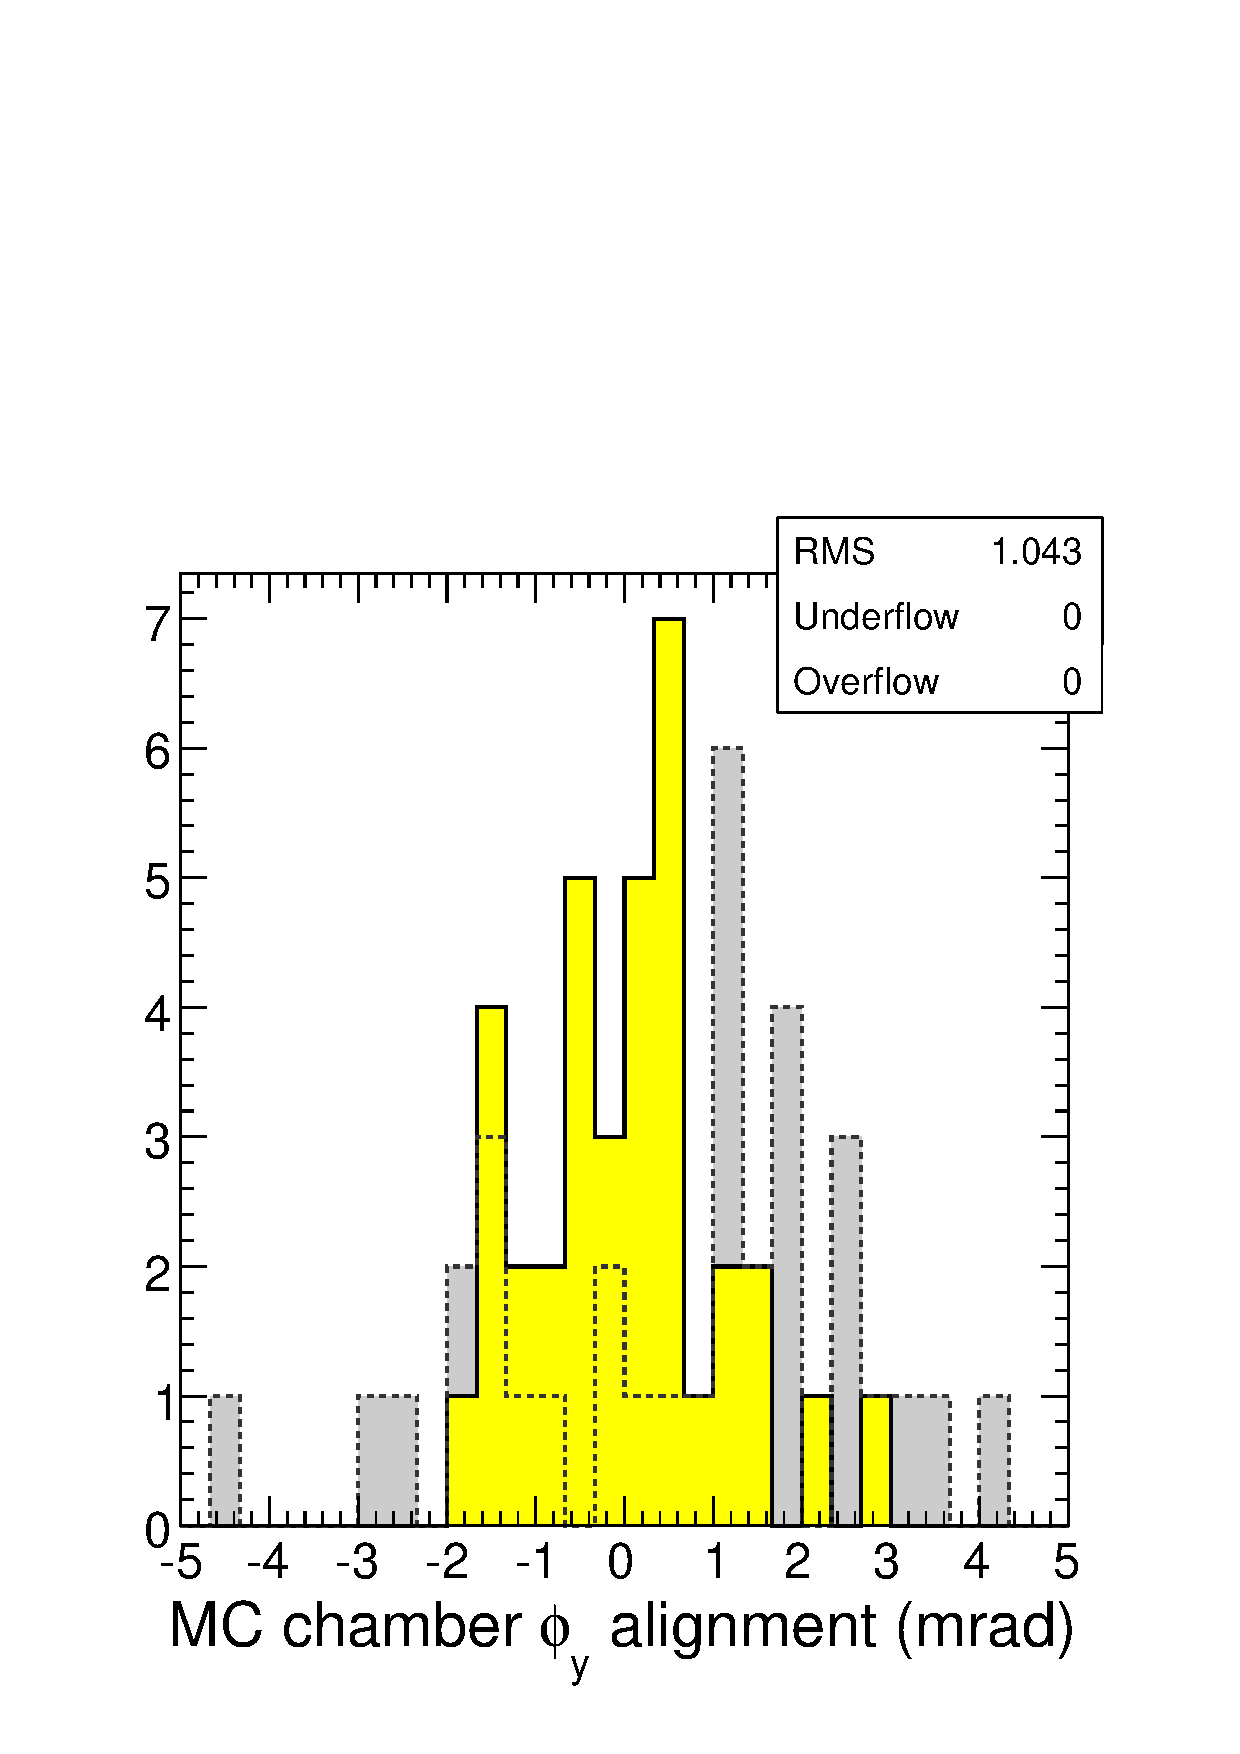
\includegraphics[width=0.5\linewidth]{mcchamber_phiy.pdf}
\end{columns}
\end{frame}

\begin{frame}
\frametitle{CSC layer misalignments}
\begin{itemize}
\item We've never modelled layer misalignments in an MC scenario before
\item They are small (0.092~mm in $x$)
\item I put this into the scenario anyway ($x$ only)
\end{itemize}

\begin{center}
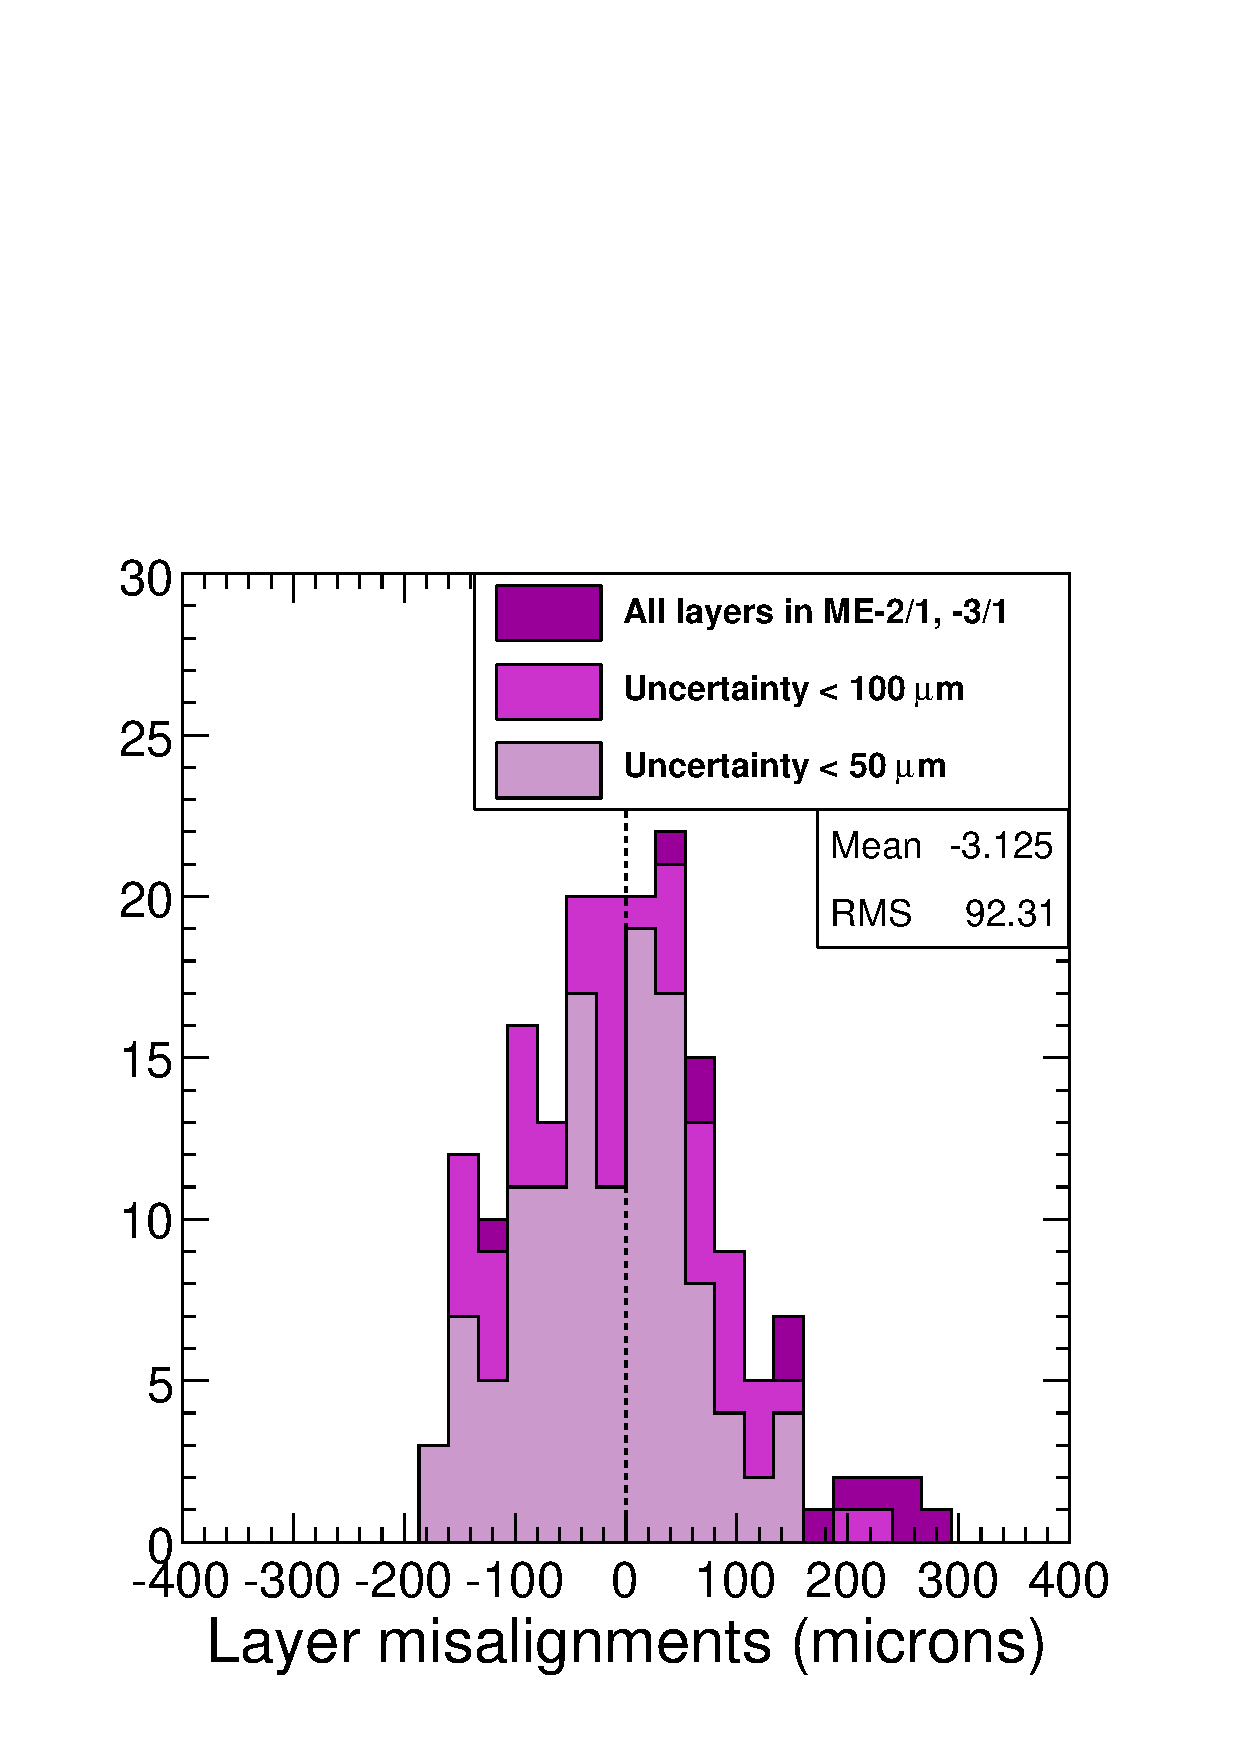
\includegraphics[width=0.45\linewidth]{layer_hist.pdf}
\end{center}
\end{frame}

\begin{frame}
\frametitle{Reference: all the constants}
\framesubtitle{Yellow denotes a parameter that was aligned with globalMuons}
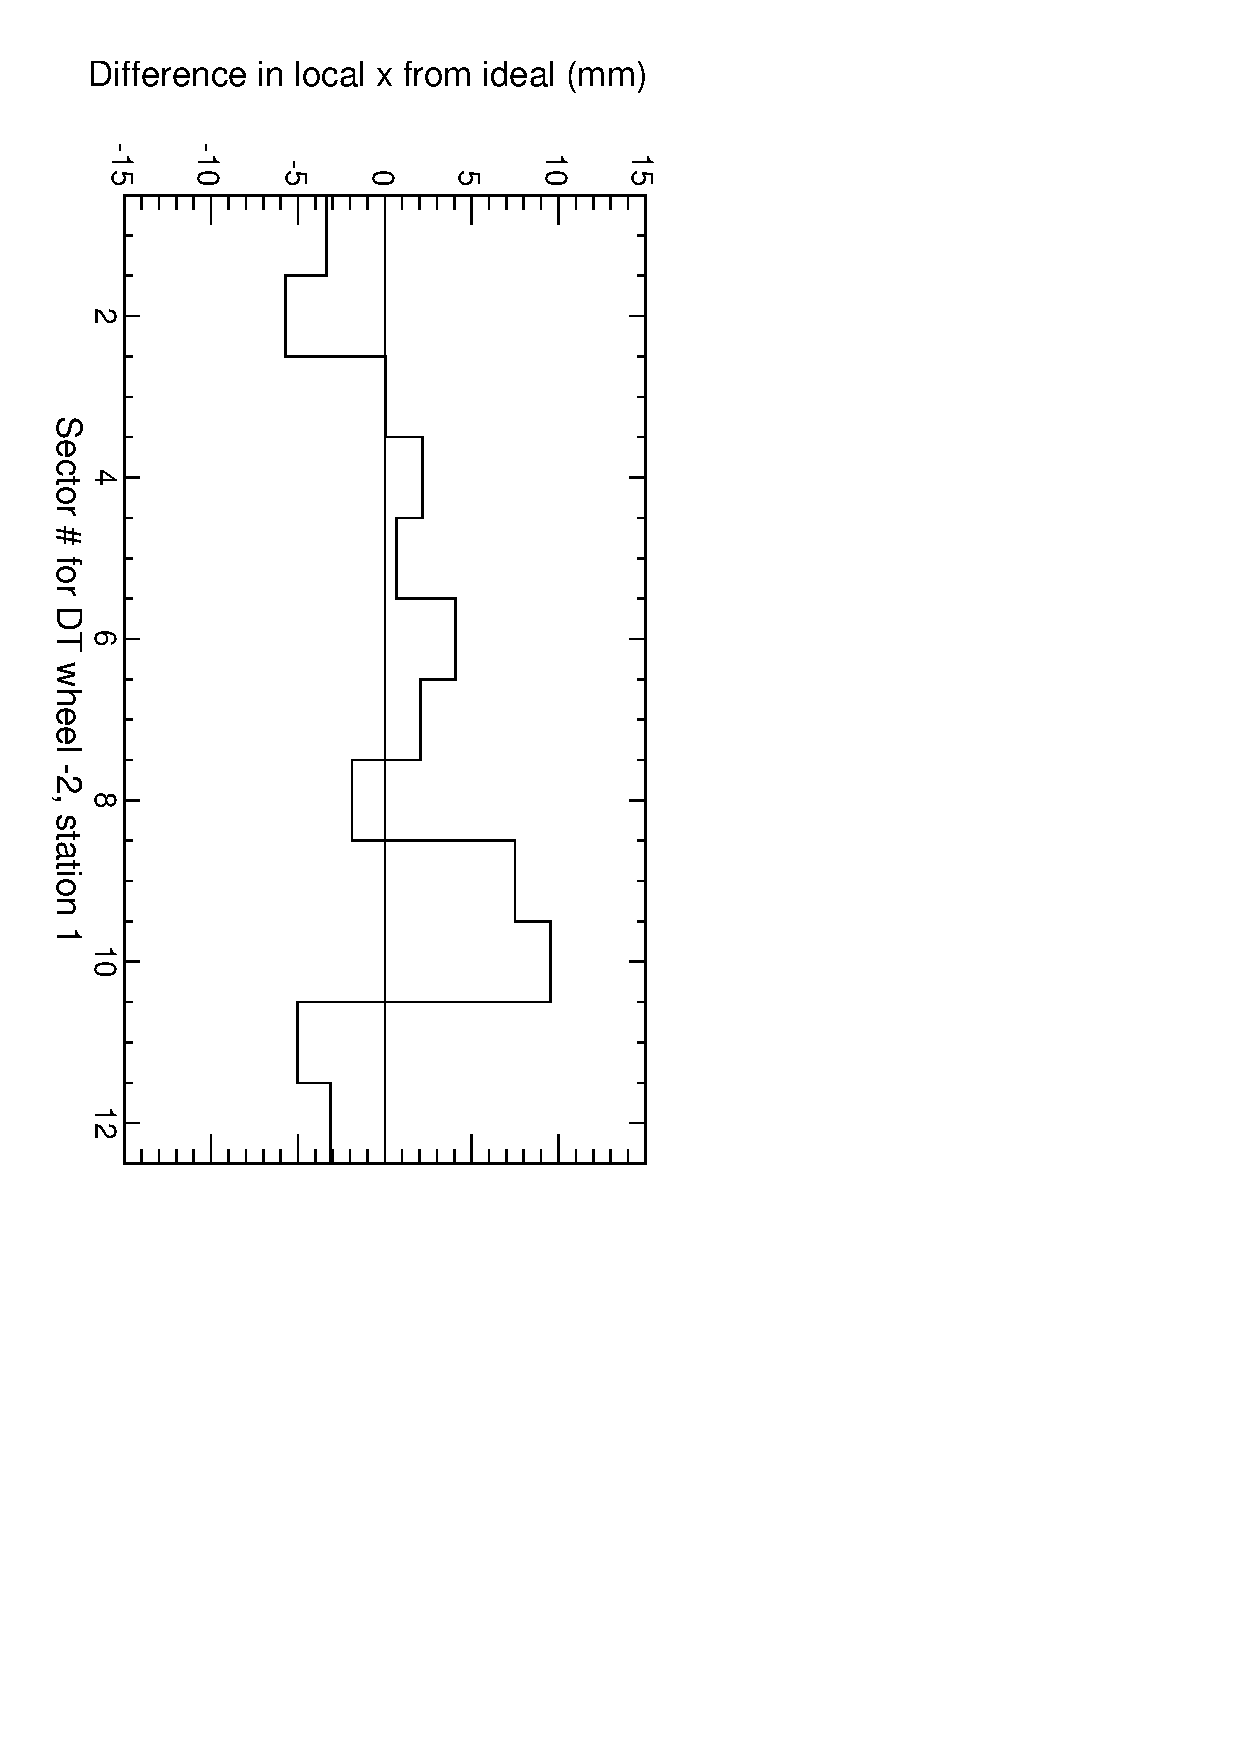
\includegraphics[height=0.5\linewidth, angle=90]{DThist000.pdf} 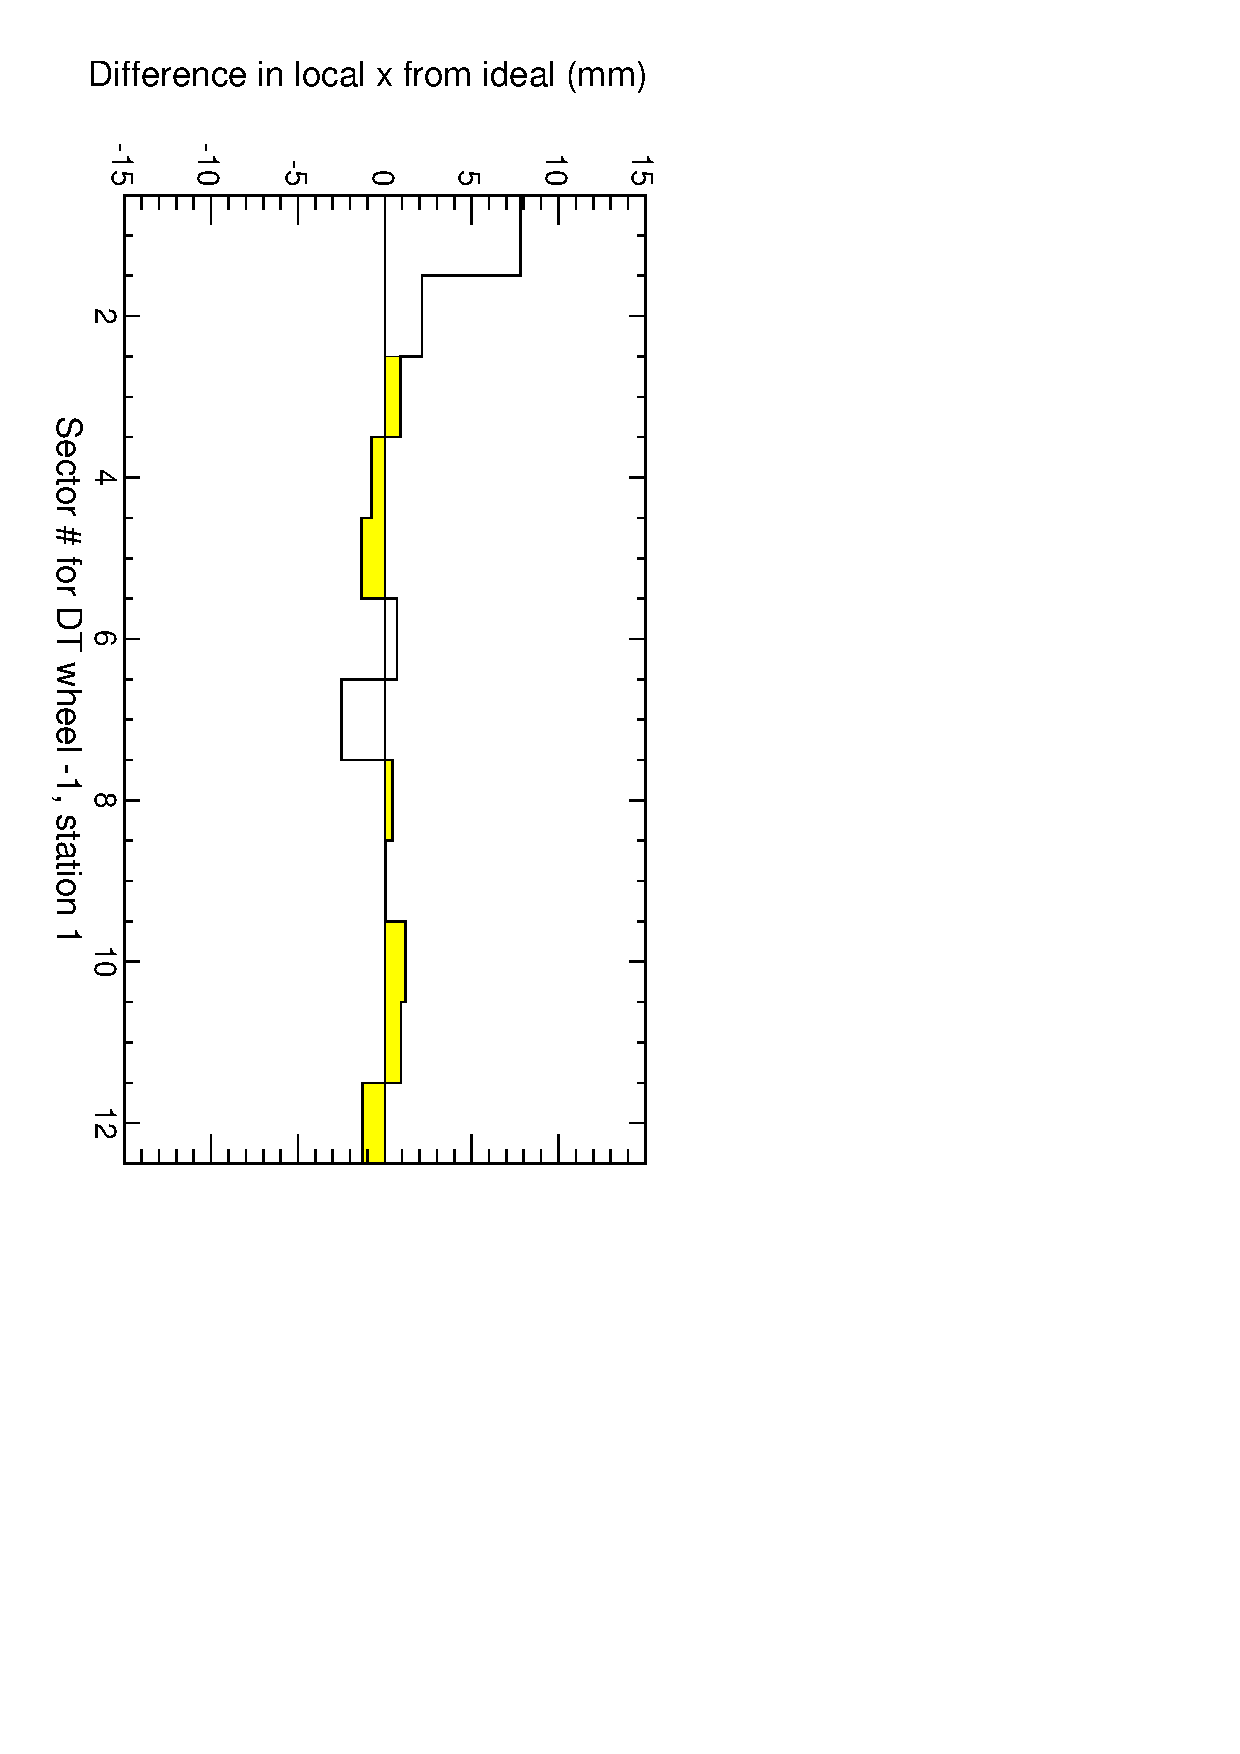
\includegraphics[height=0.5\linewidth, angle=90]{DThist001.pdf} \\
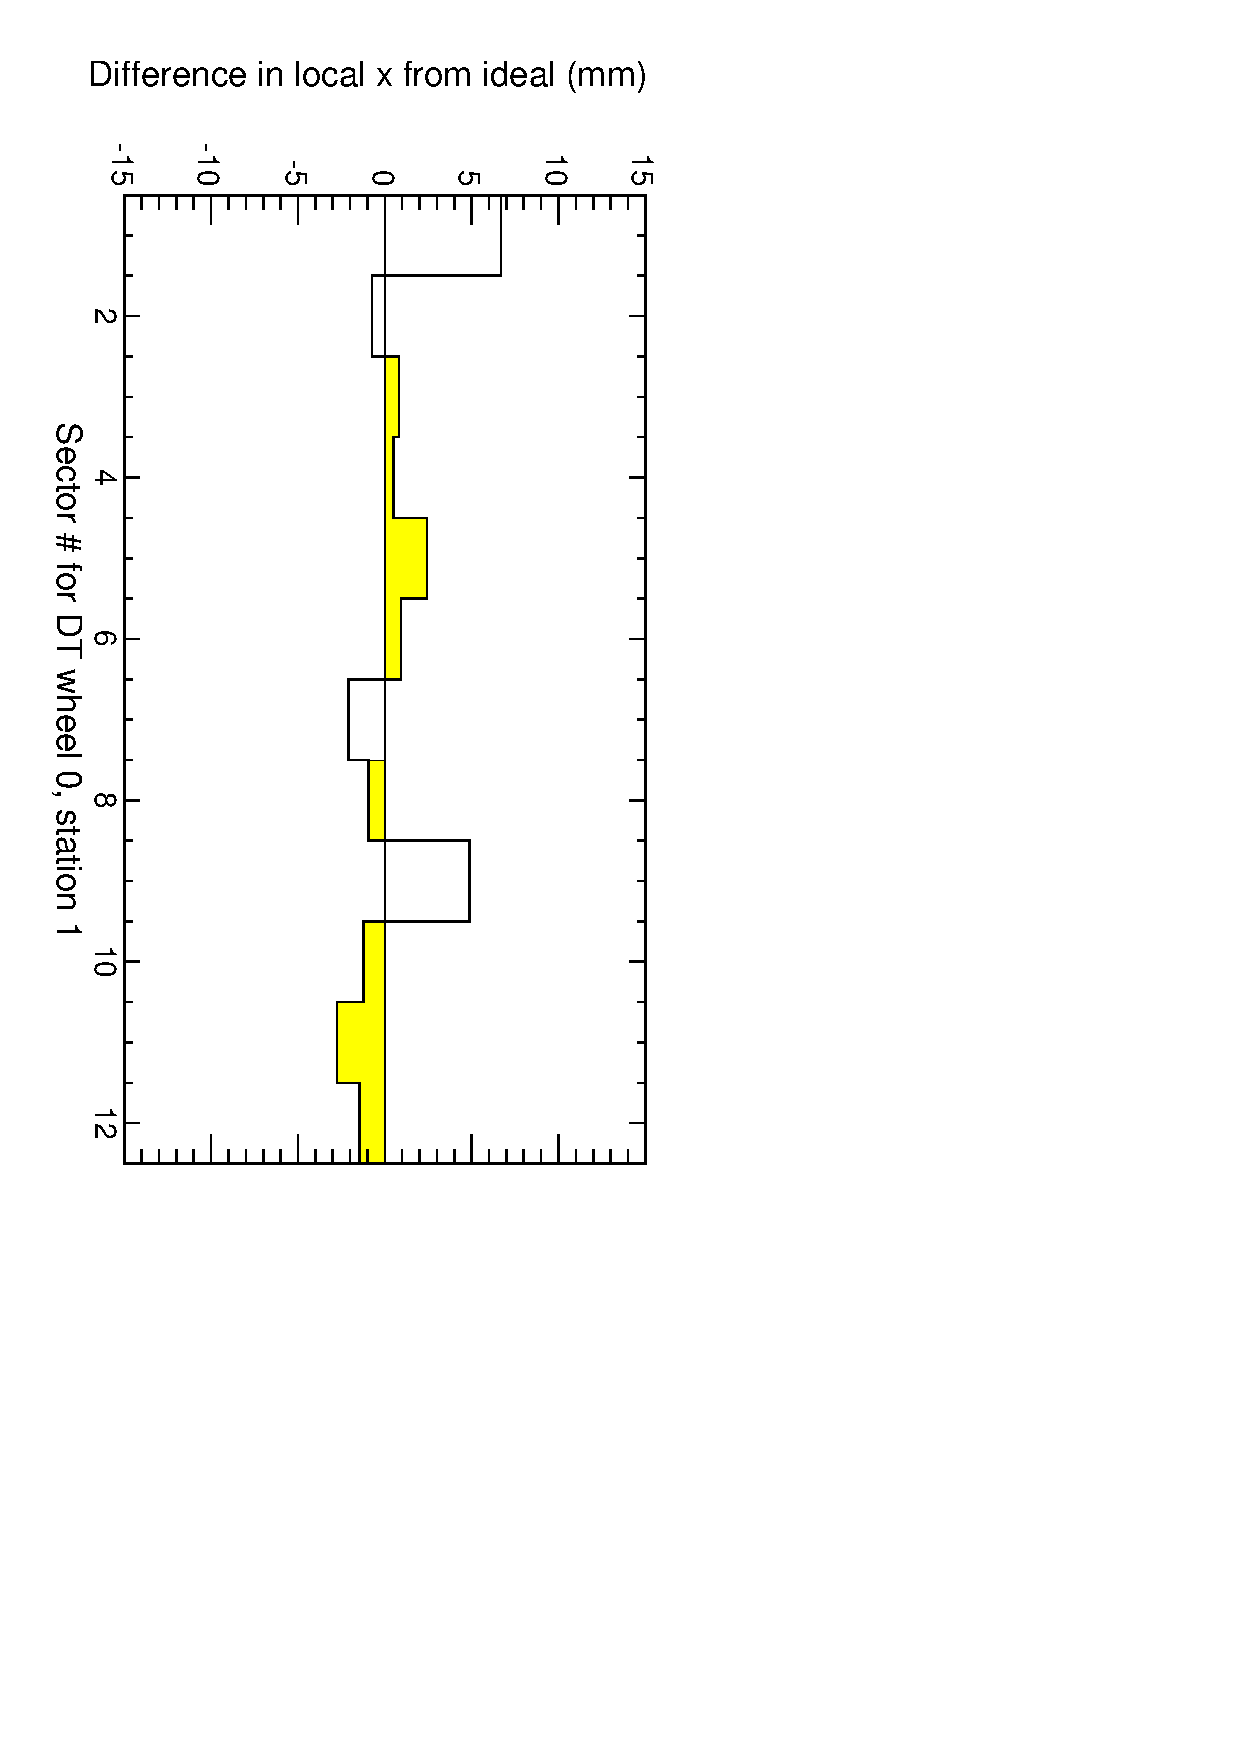
\includegraphics[height=0.5\linewidth, angle=90]{DThist002.pdf} 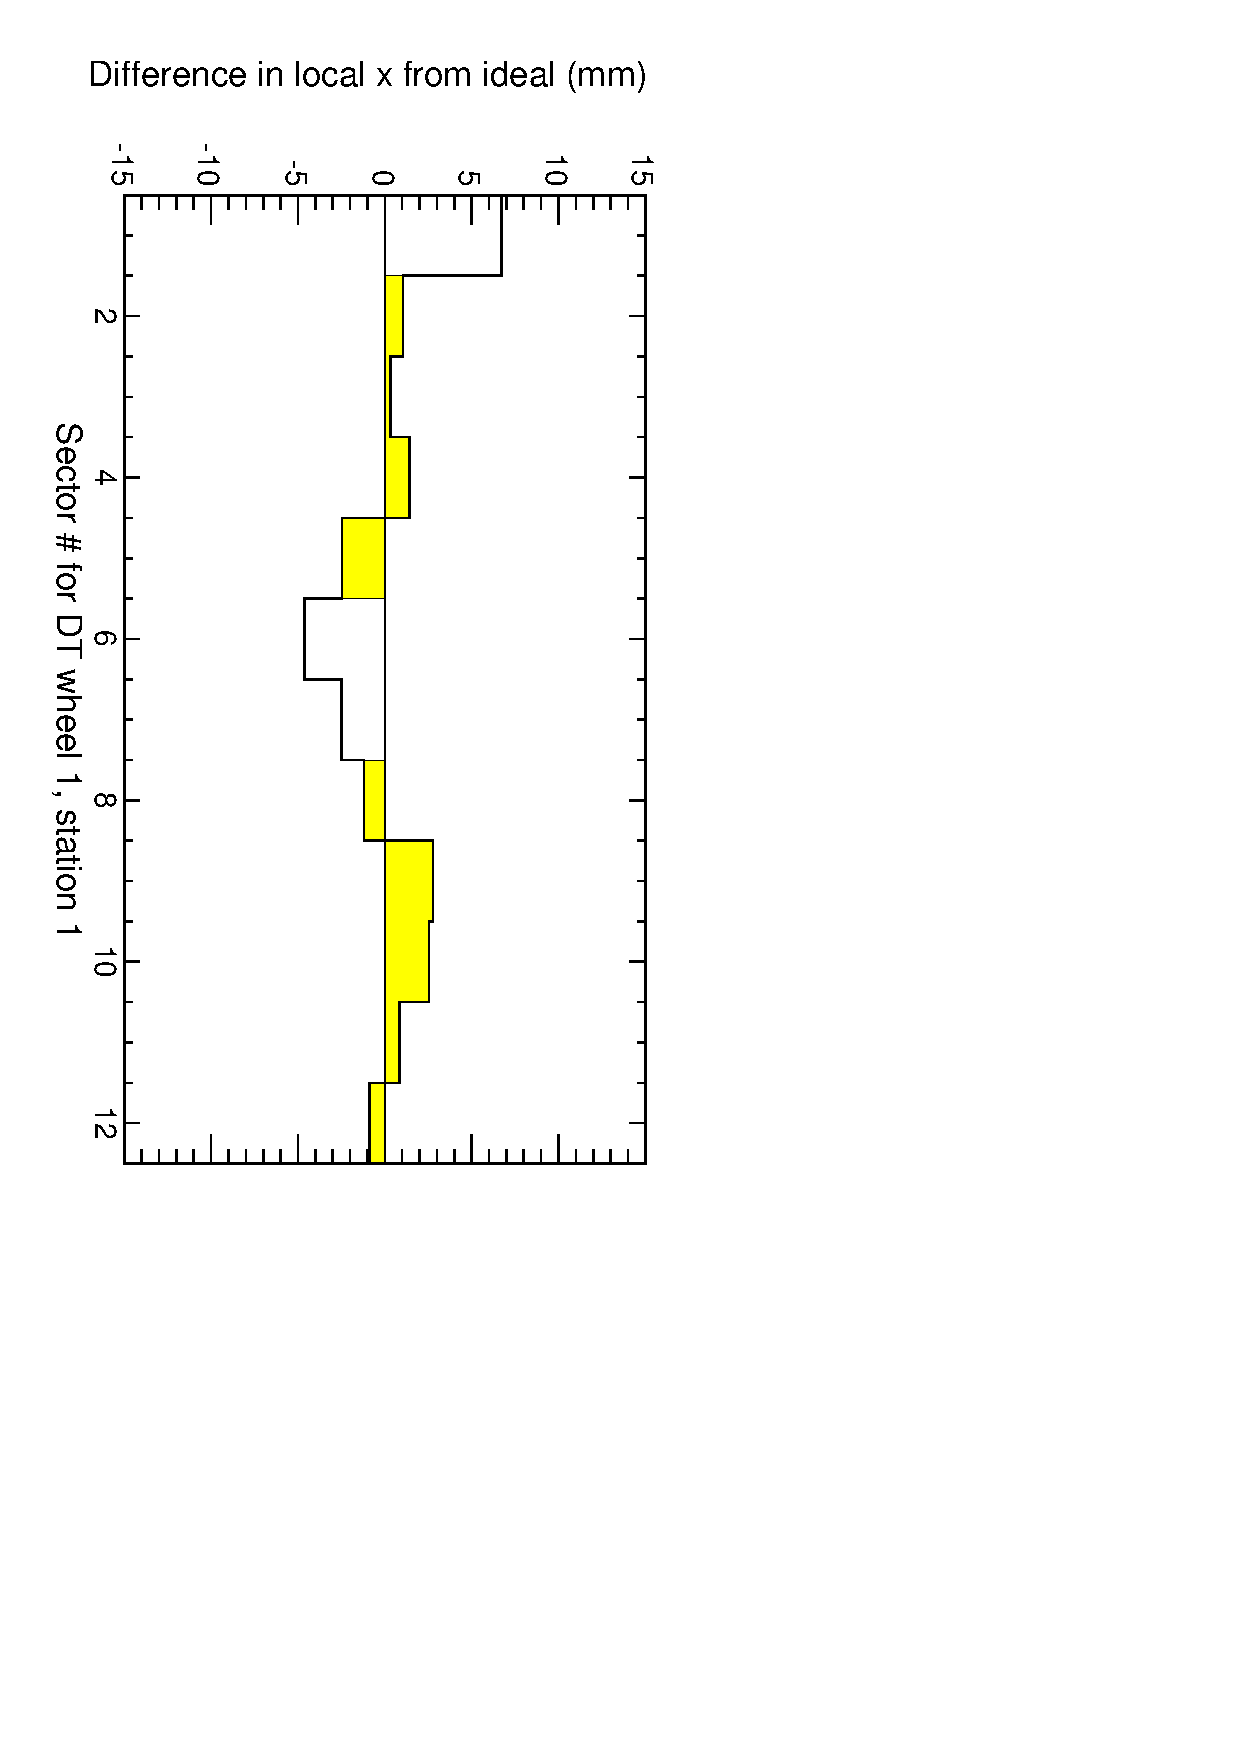
\includegraphics[height=0.5\linewidth, angle=90]{DThist003.pdf}
\end{frame}

\begin{frame}
\frametitle{Reference: all the constants}
\framesubtitle{Yellow denotes a parameter that was aligned with globalMuons}
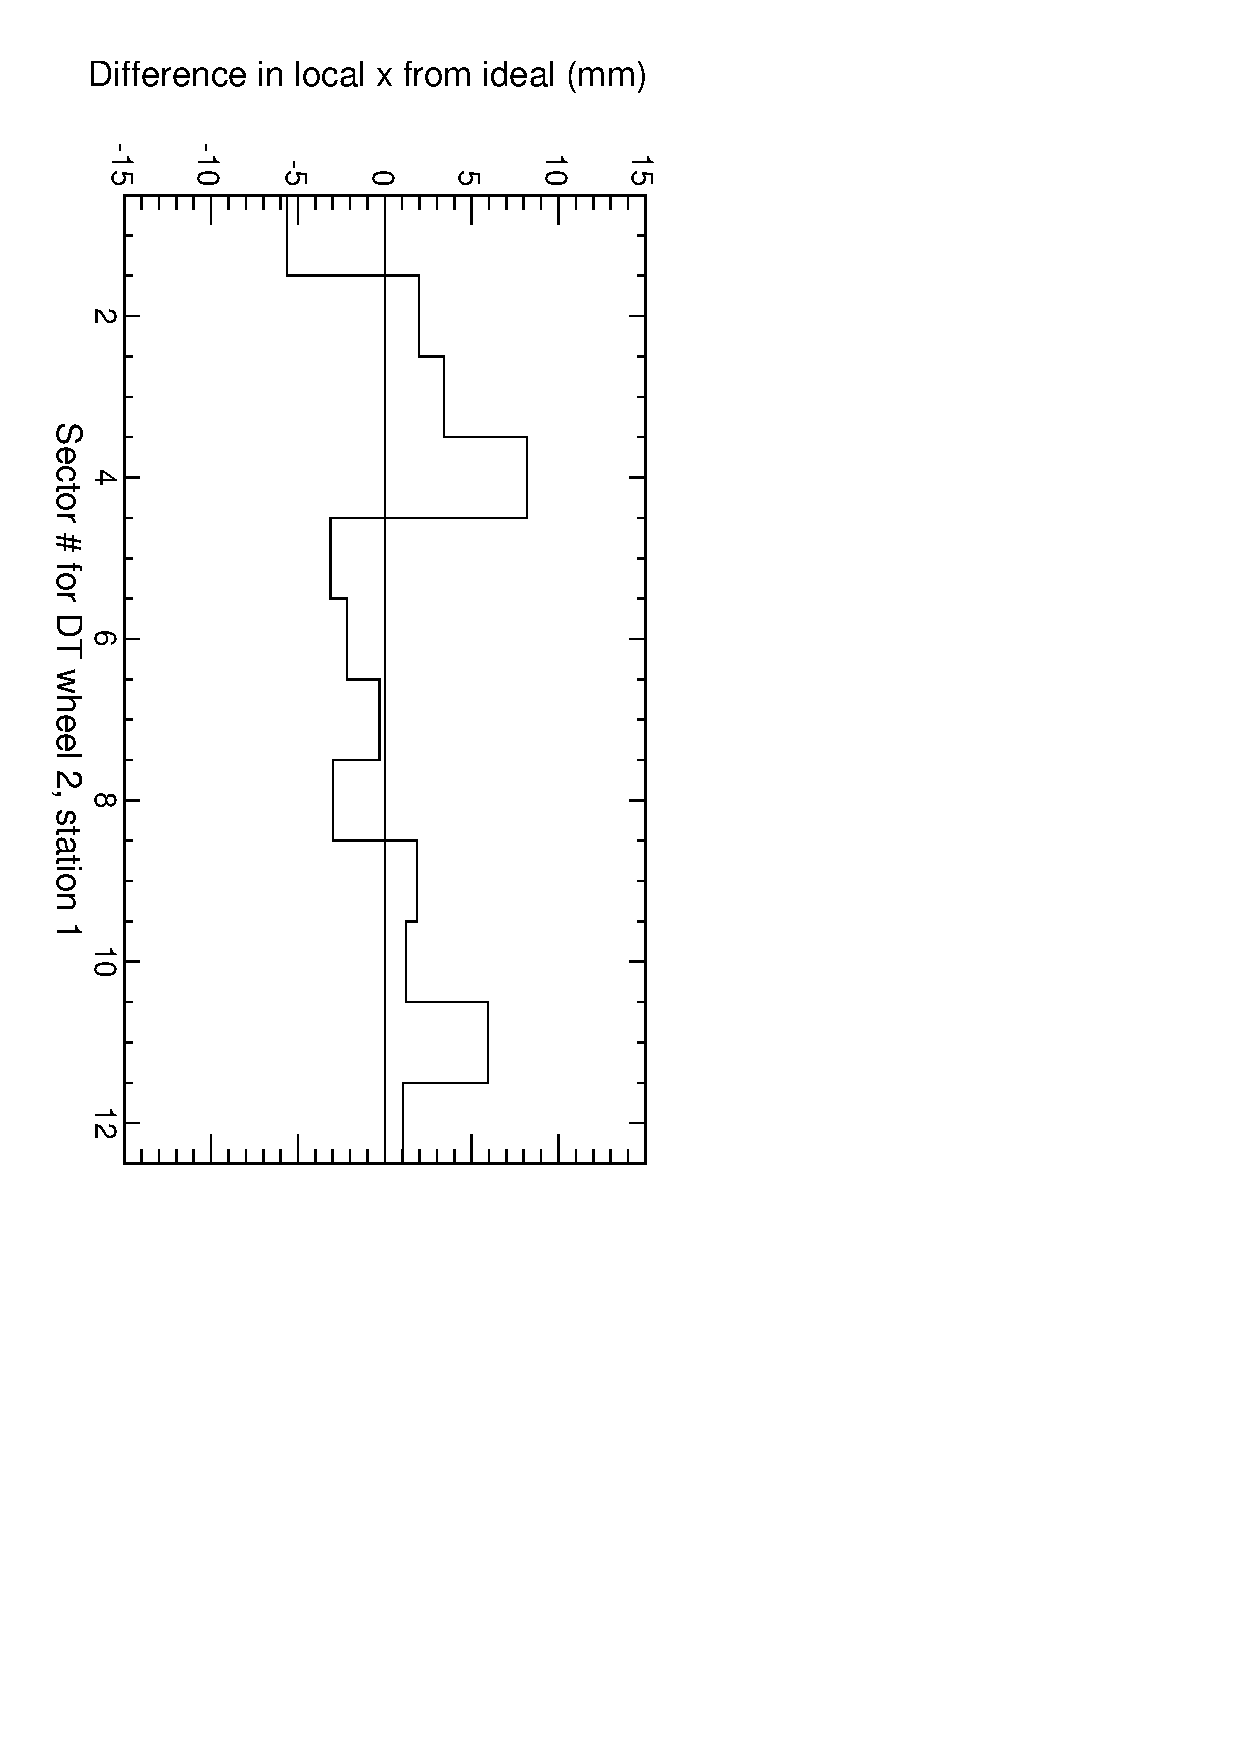
\includegraphics[height=0.5\linewidth, angle=90]{DThist004.pdf} 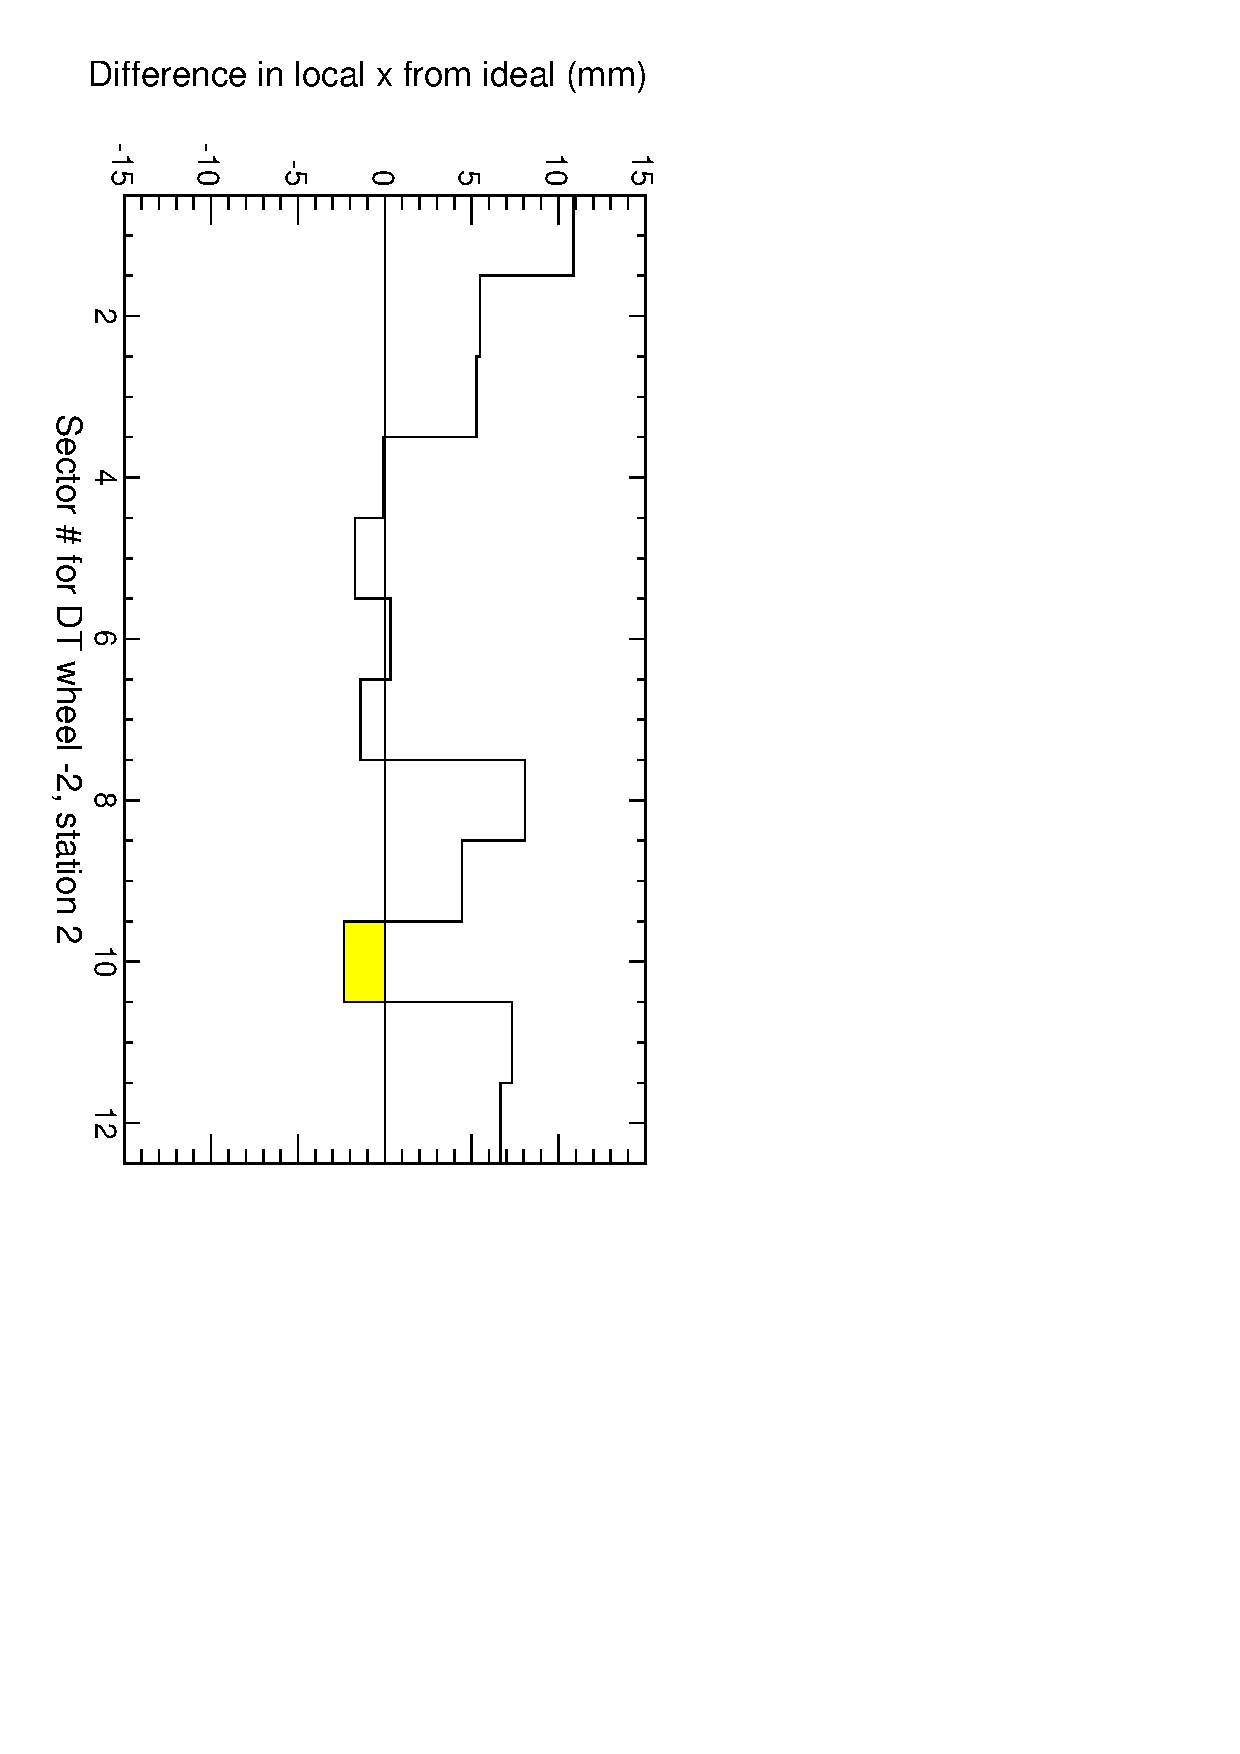
\includegraphics[height=0.5\linewidth, angle=90]{DThist005.pdf} \\
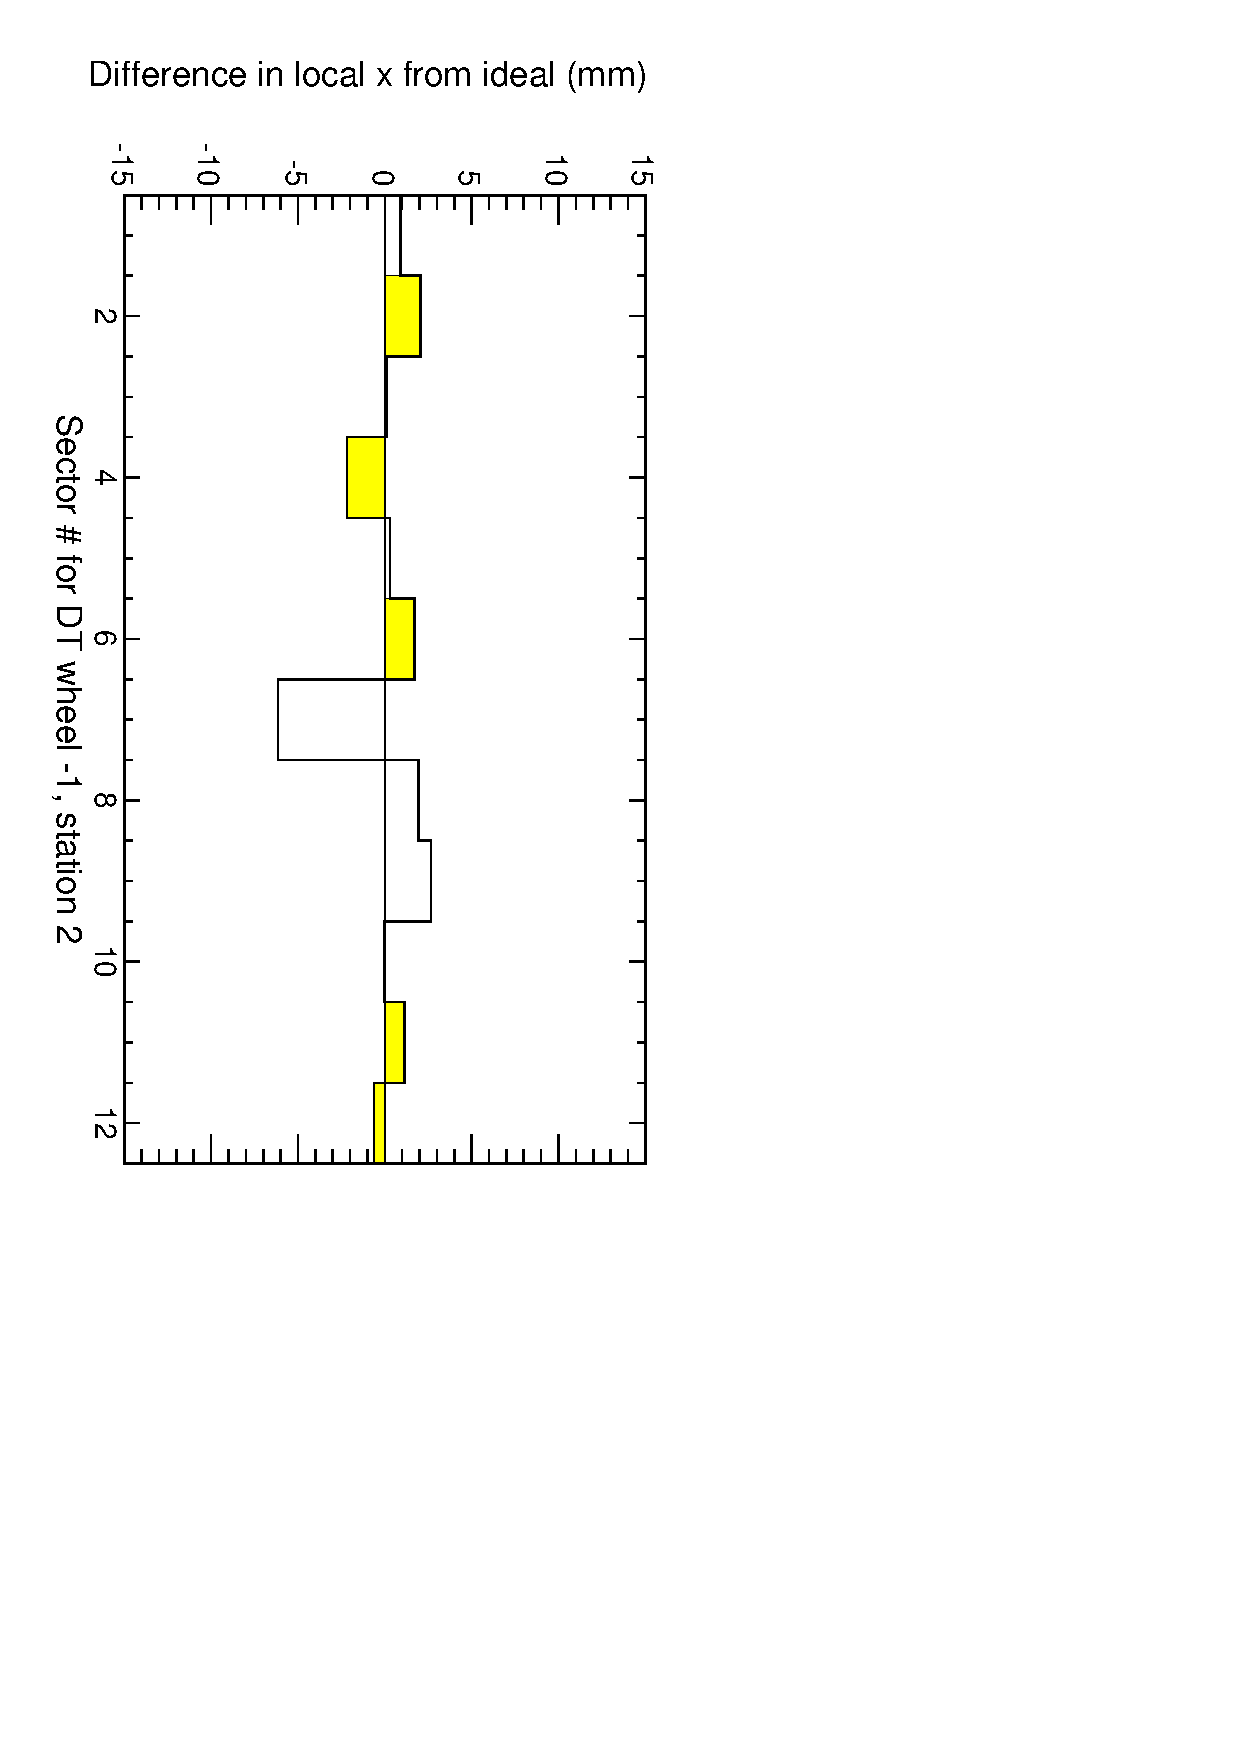
\includegraphics[height=0.5\linewidth, angle=90]{DThist006.pdf} 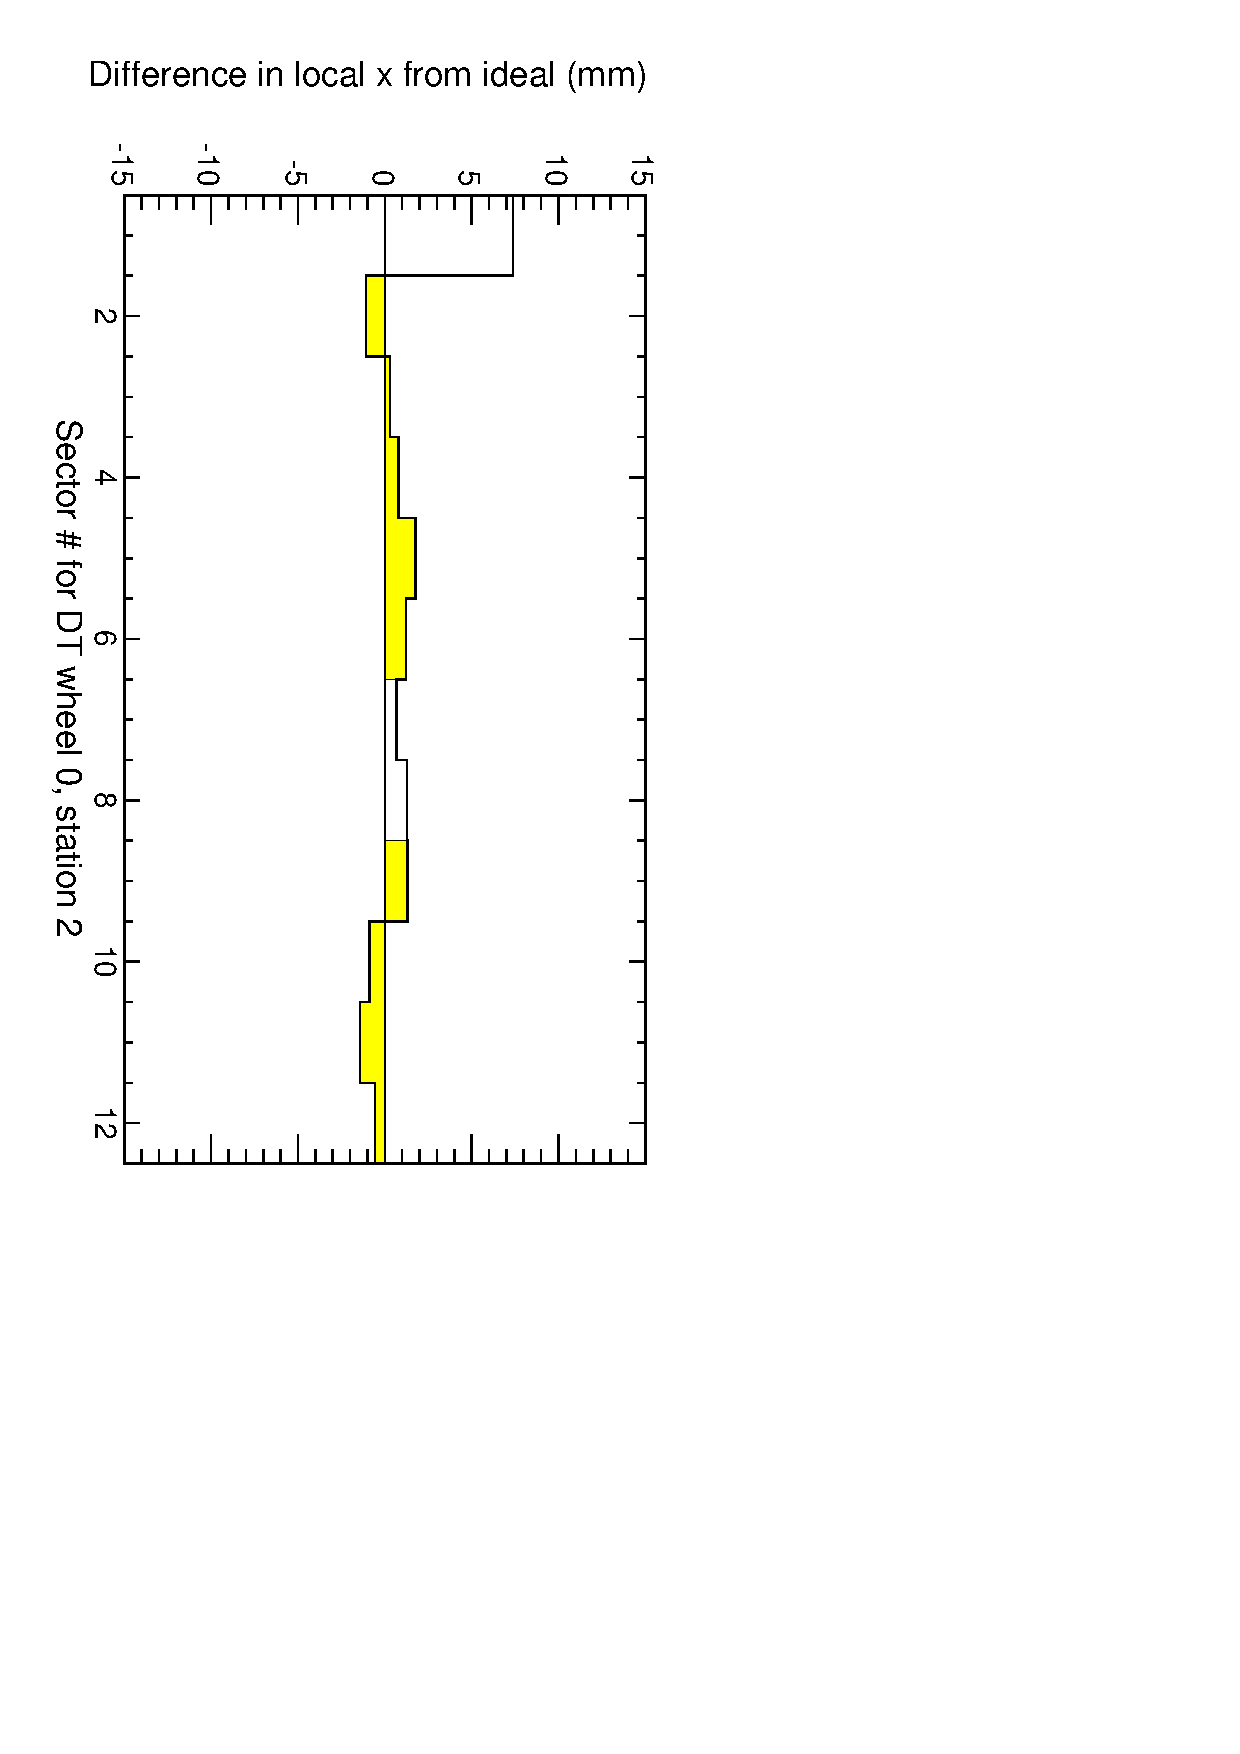
\includegraphics[height=0.5\linewidth, angle=90]{DThist007.pdf}
\end{frame}

\begin{frame}
\frametitle{Reference: all the constants}
\framesubtitle{Yellow denotes a parameter that was aligned with globalMuons}
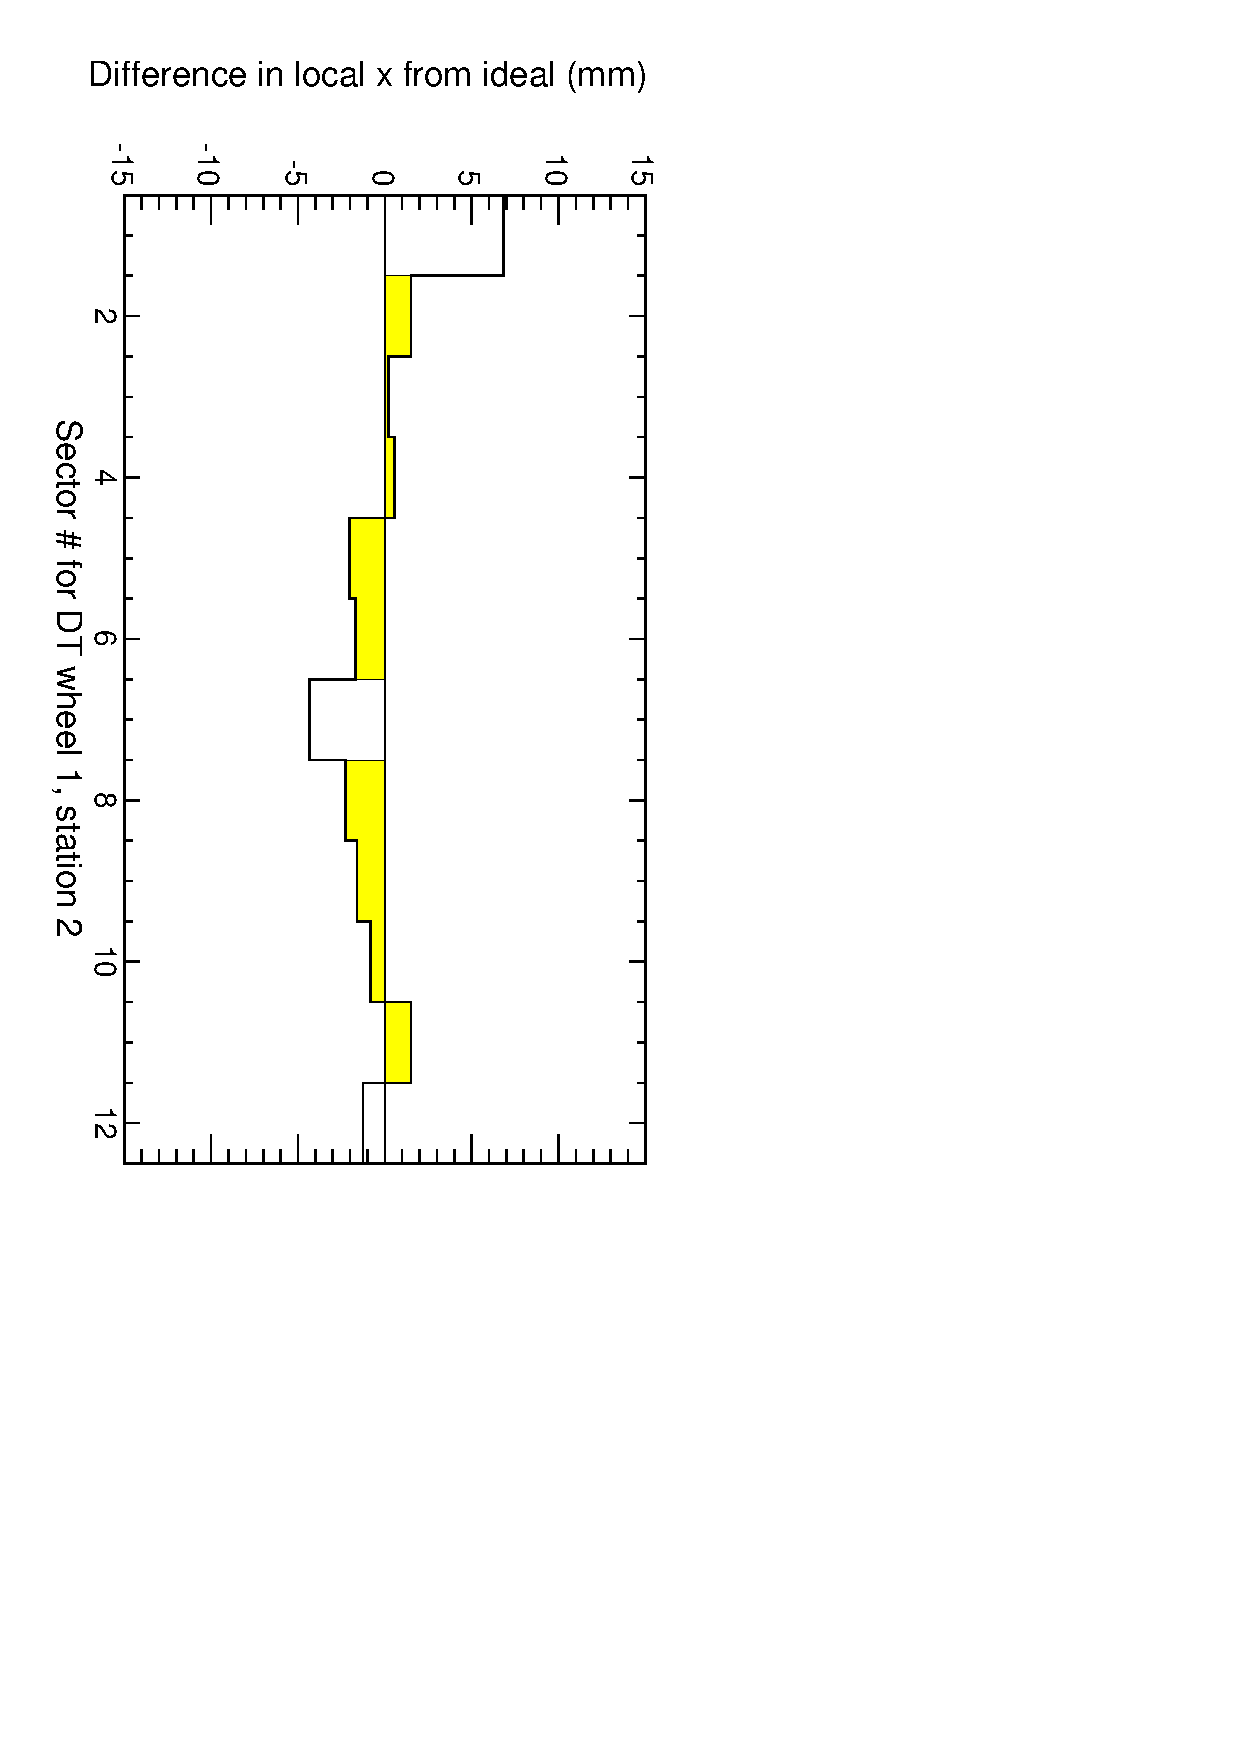
\includegraphics[height=0.5\linewidth, angle=90]{DThist008.pdf} 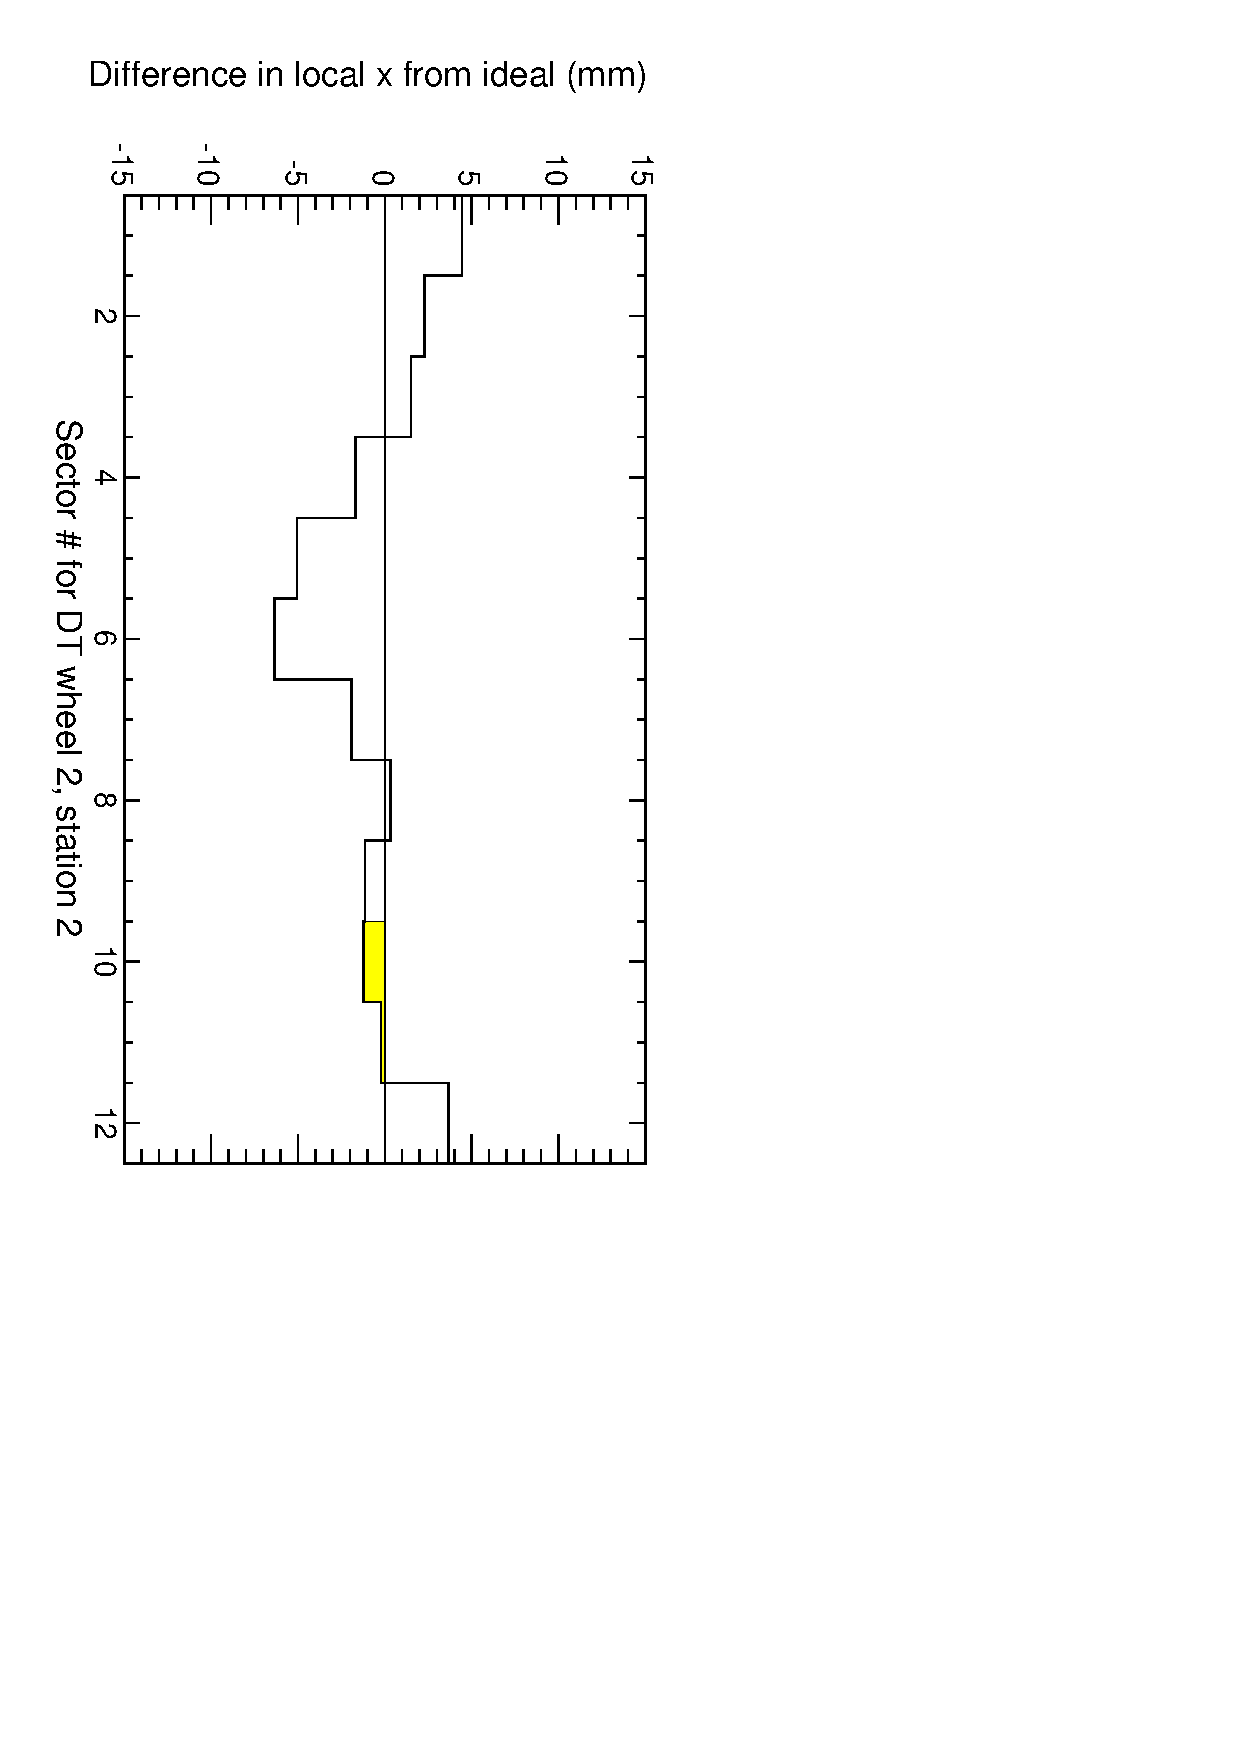
\includegraphics[height=0.5\linewidth, angle=90]{DThist009.pdf} \\
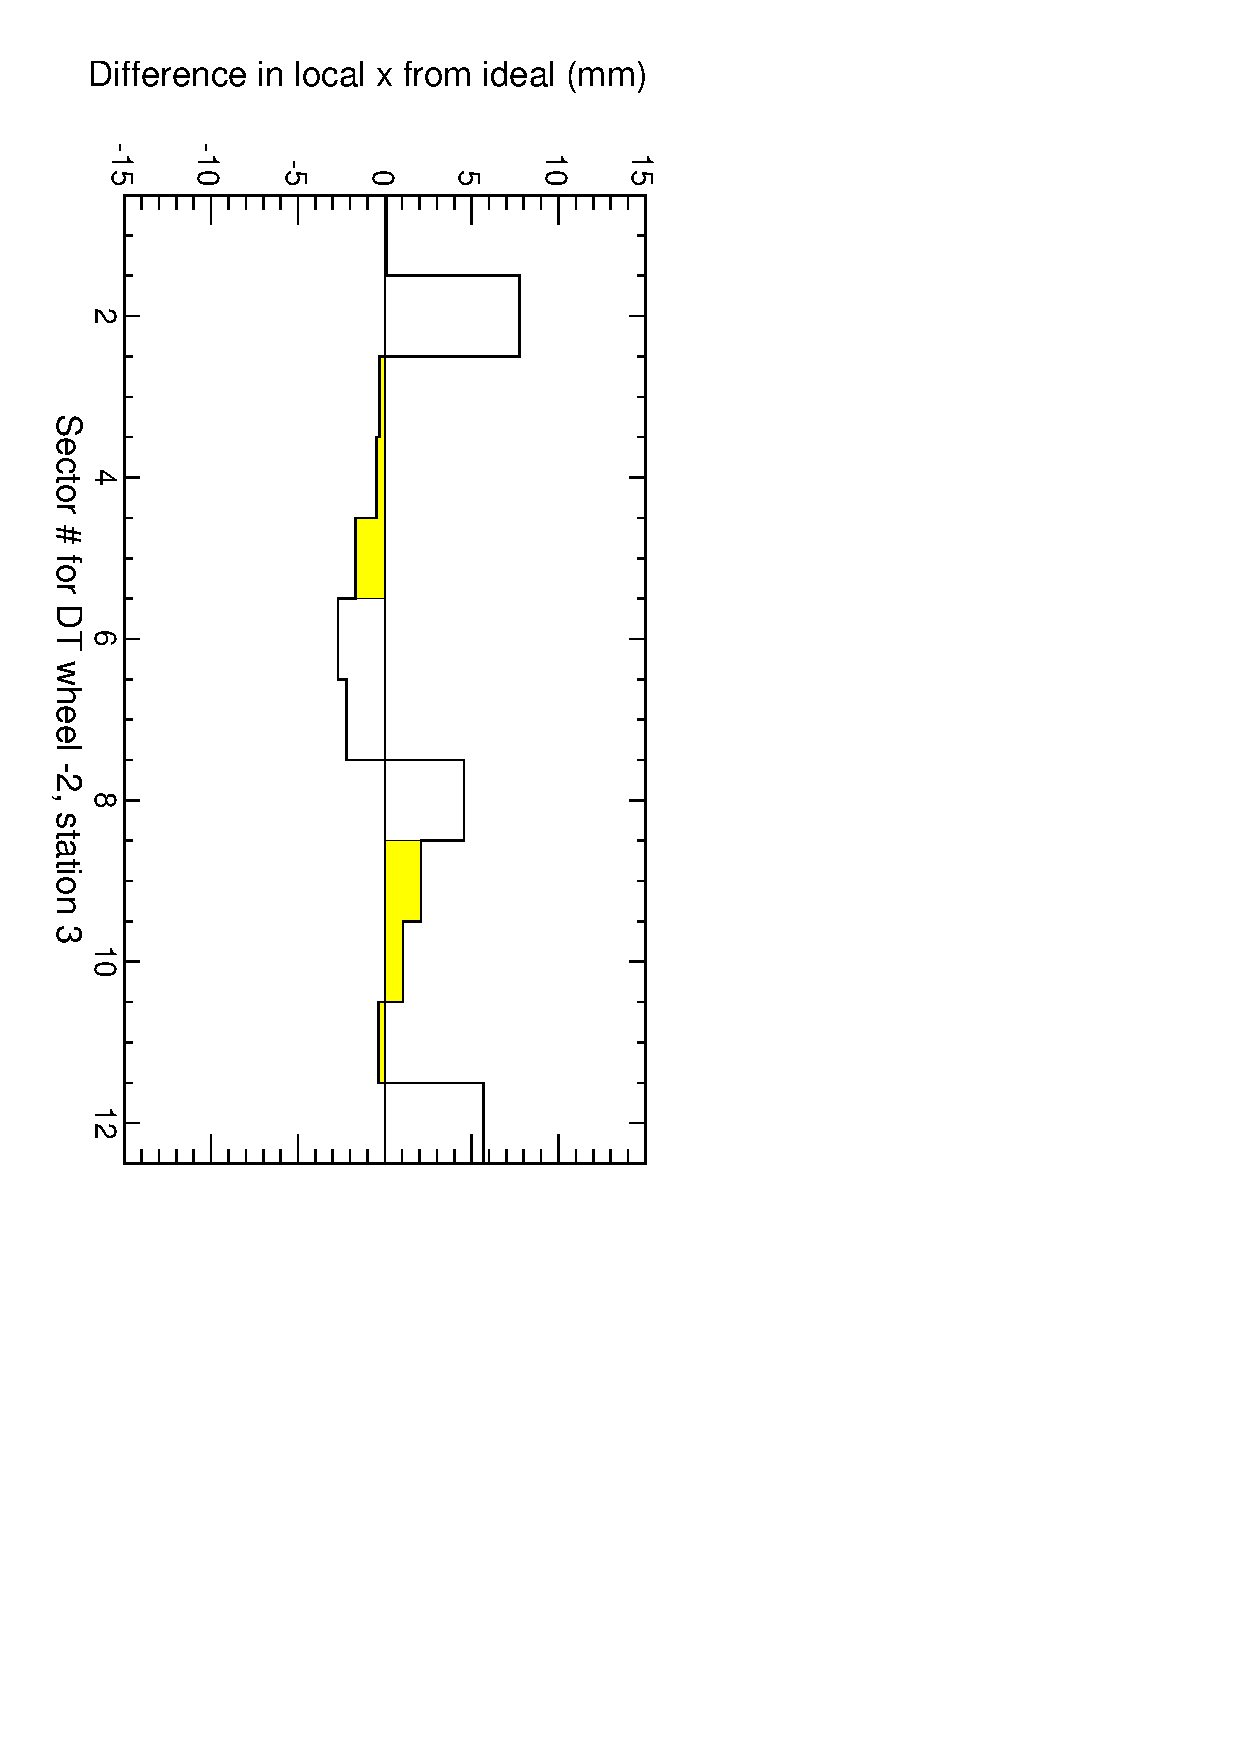
\includegraphics[height=0.5\linewidth, angle=90]{DThist010.pdf} 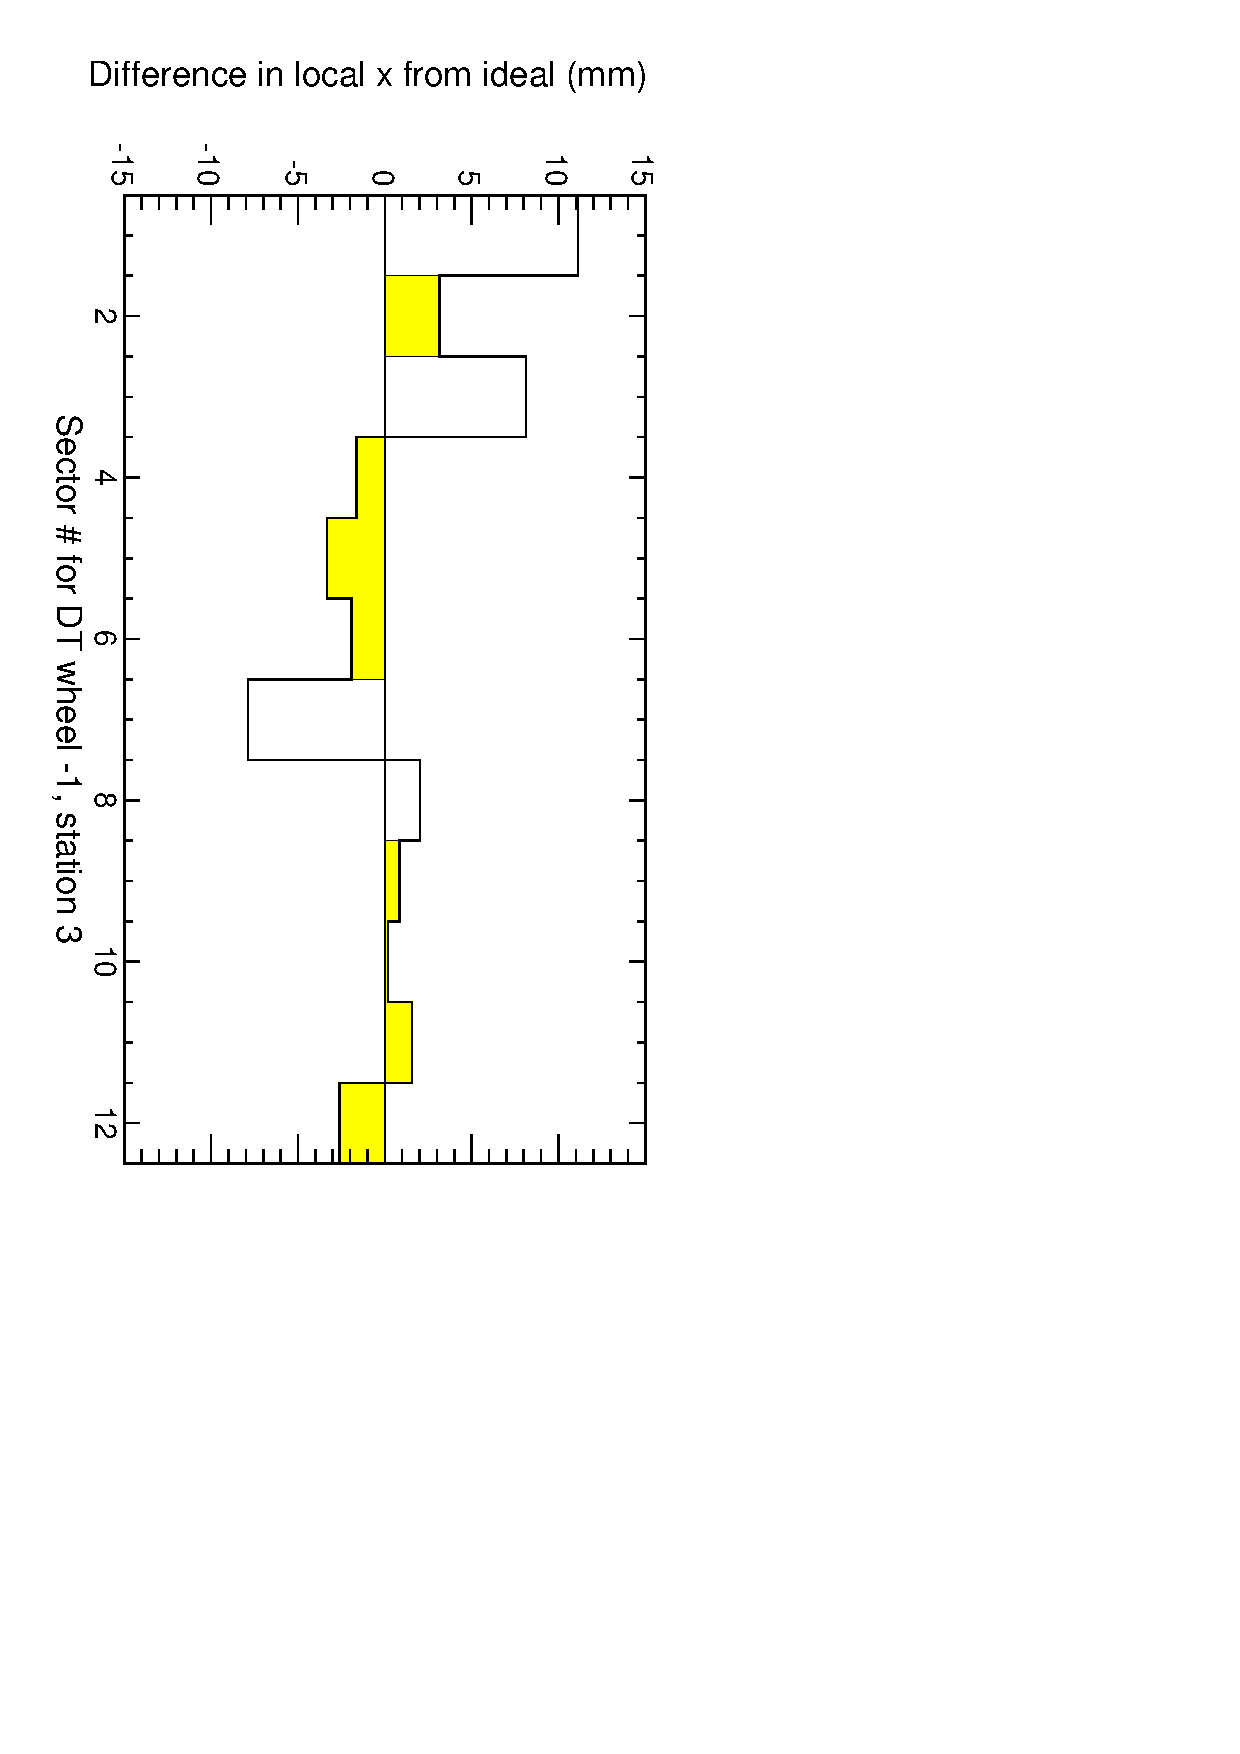
\includegraphics[height=0.5\linewidth, angle=90]{DThist011.pdf}
\end{frame}

\begin{frame}
\frametitle{Reference: all the constants}
\framesubtitle{Yellow denotes a parameter that was aligned with globalMuons}
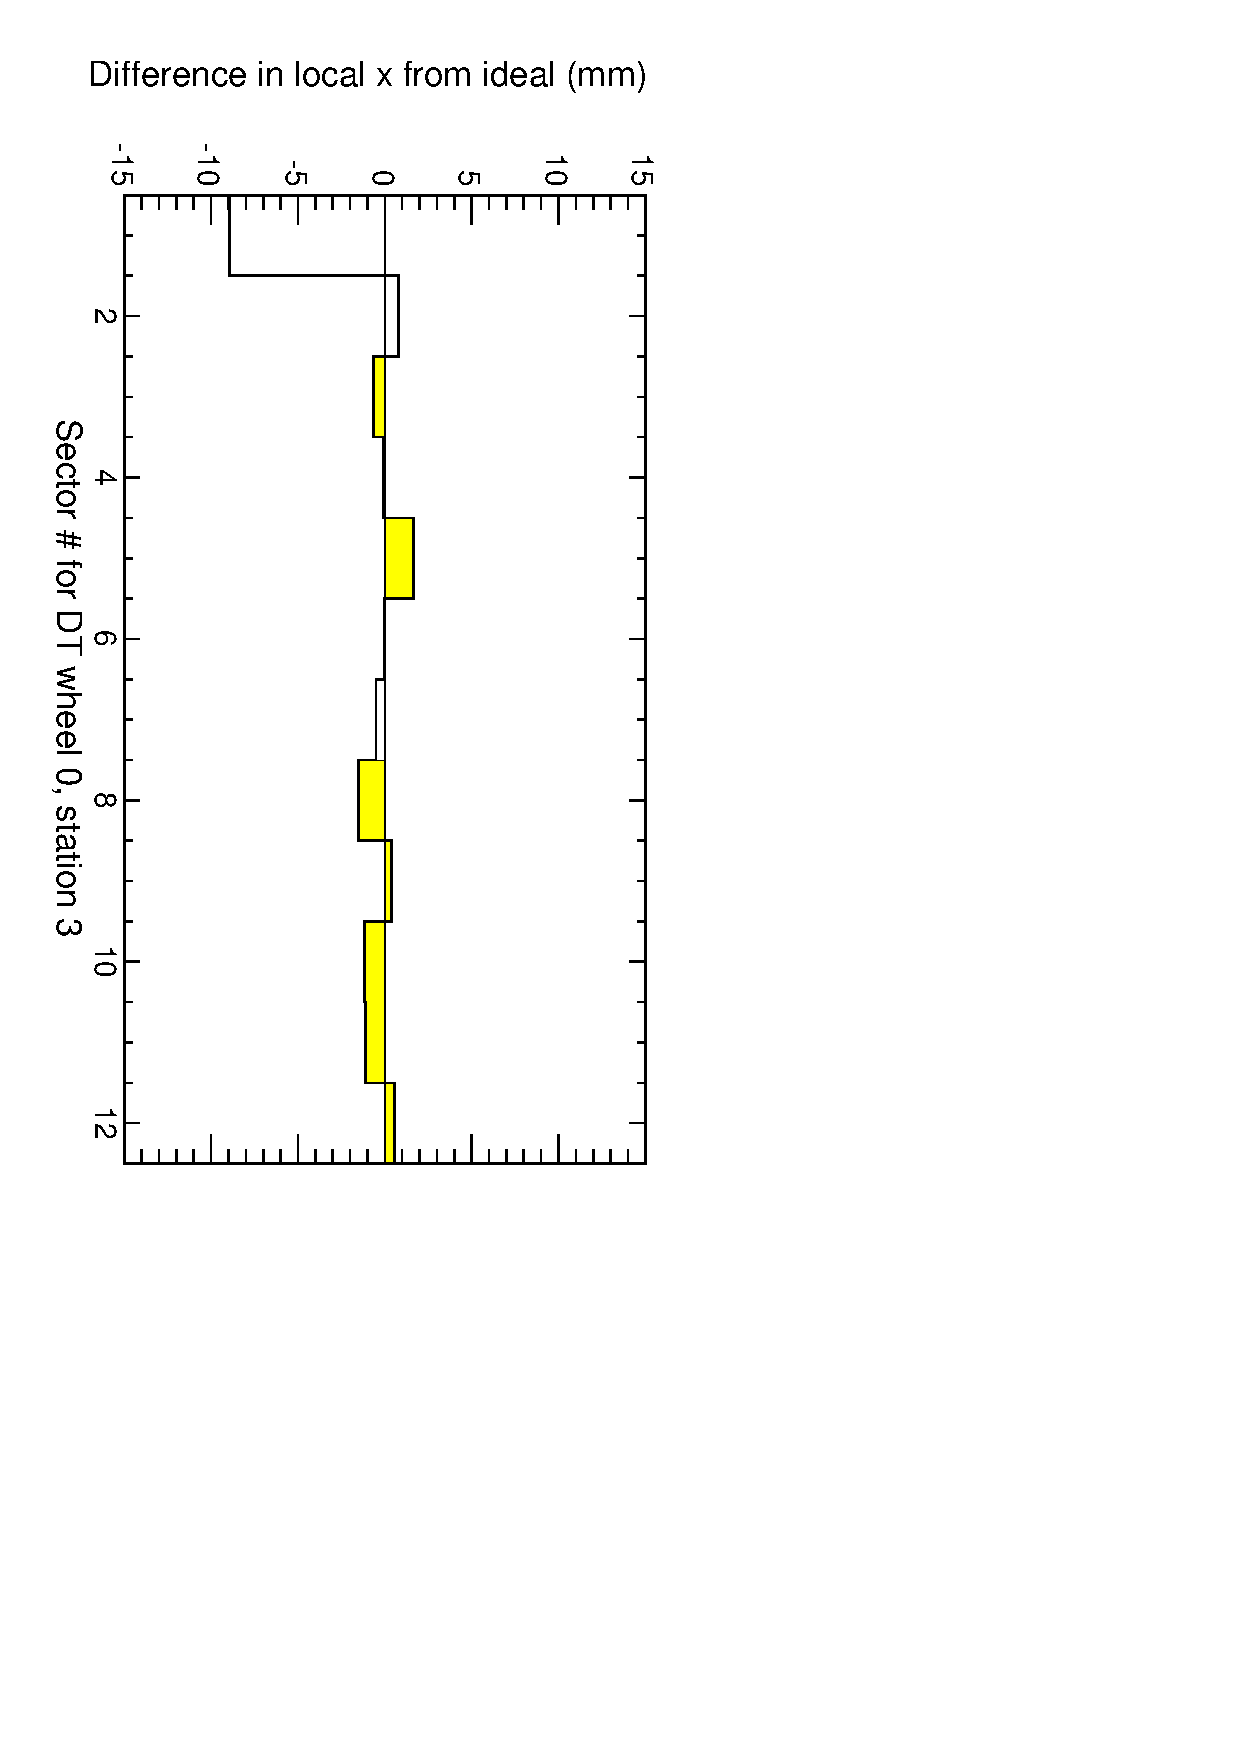
\includegraphics[height=0.5\linewidth, angle=90]{DThist012.pdf} 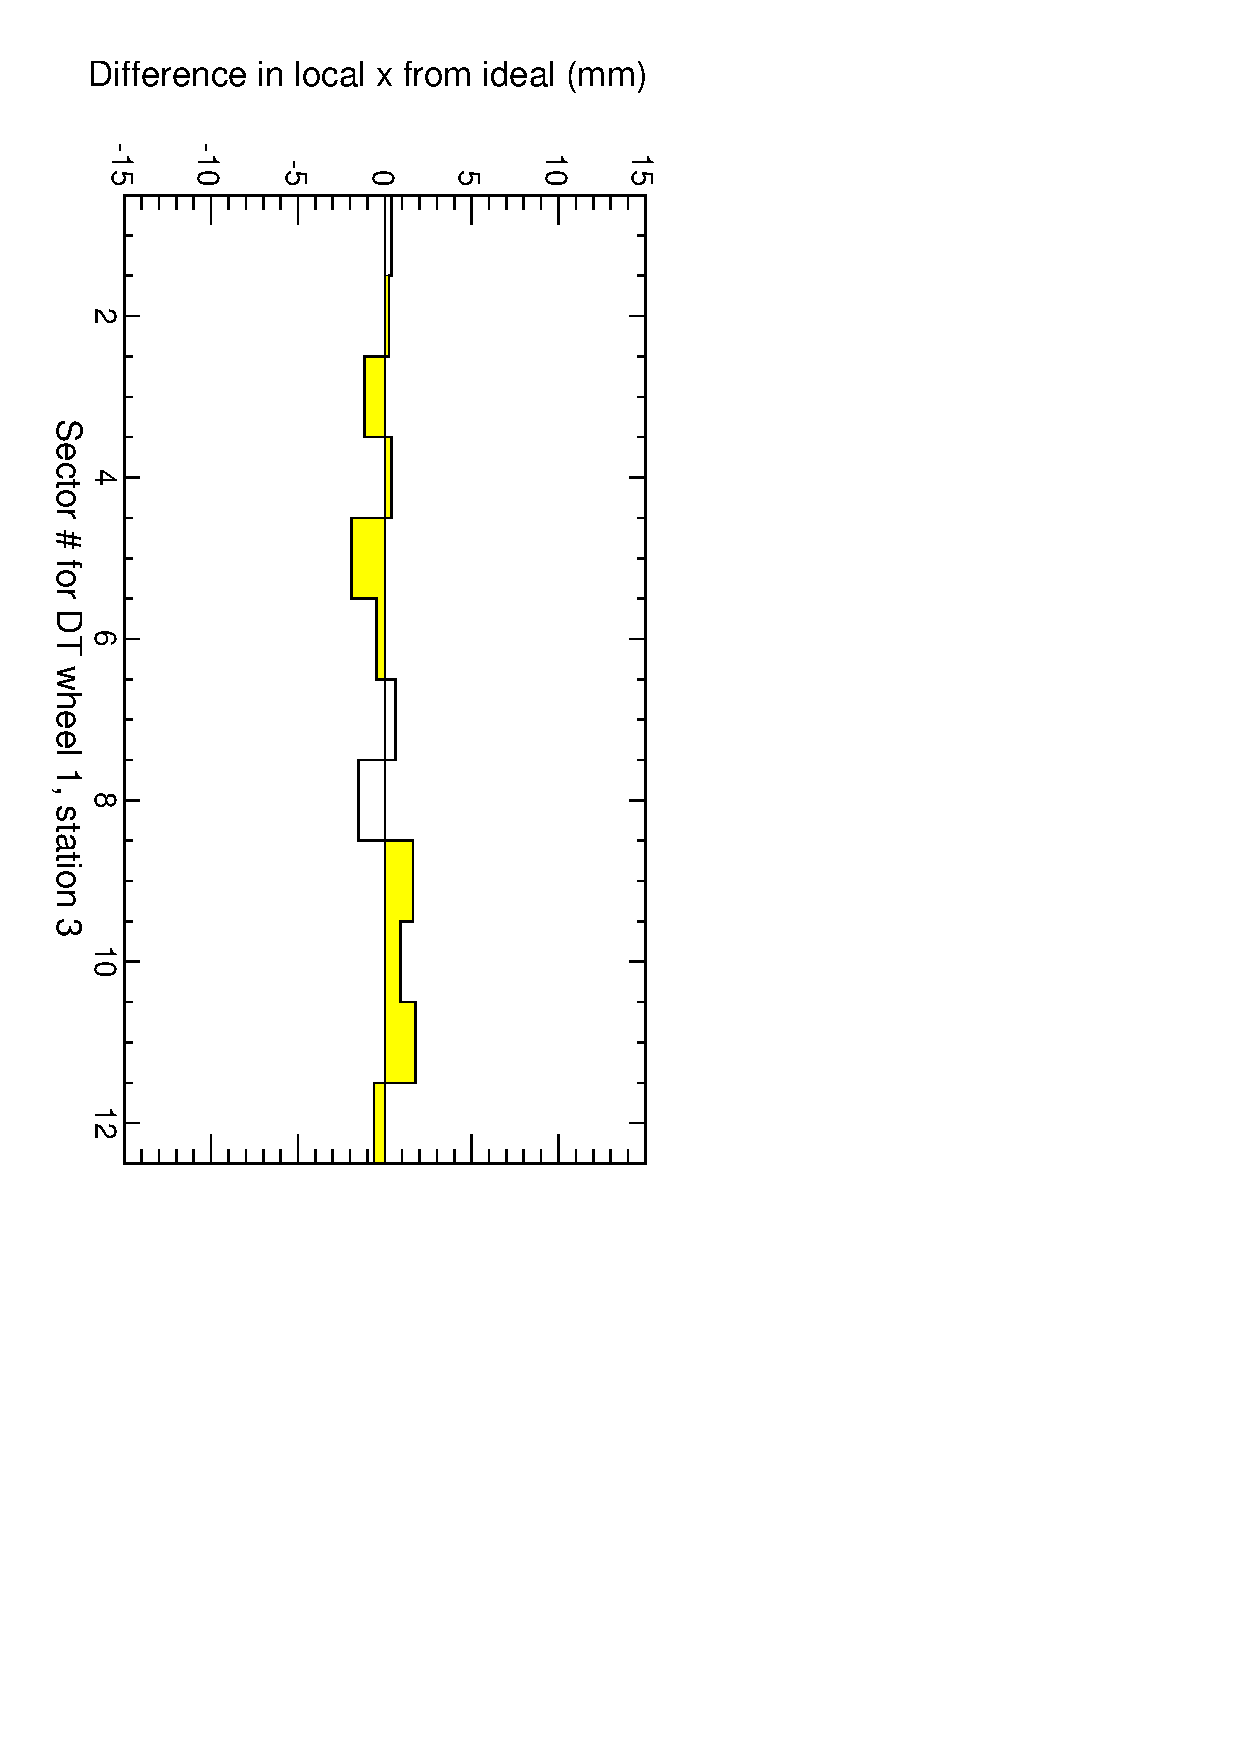
\includegraphics[height=0.5\linewidth, angle=90]{DThist013.pdf} \\
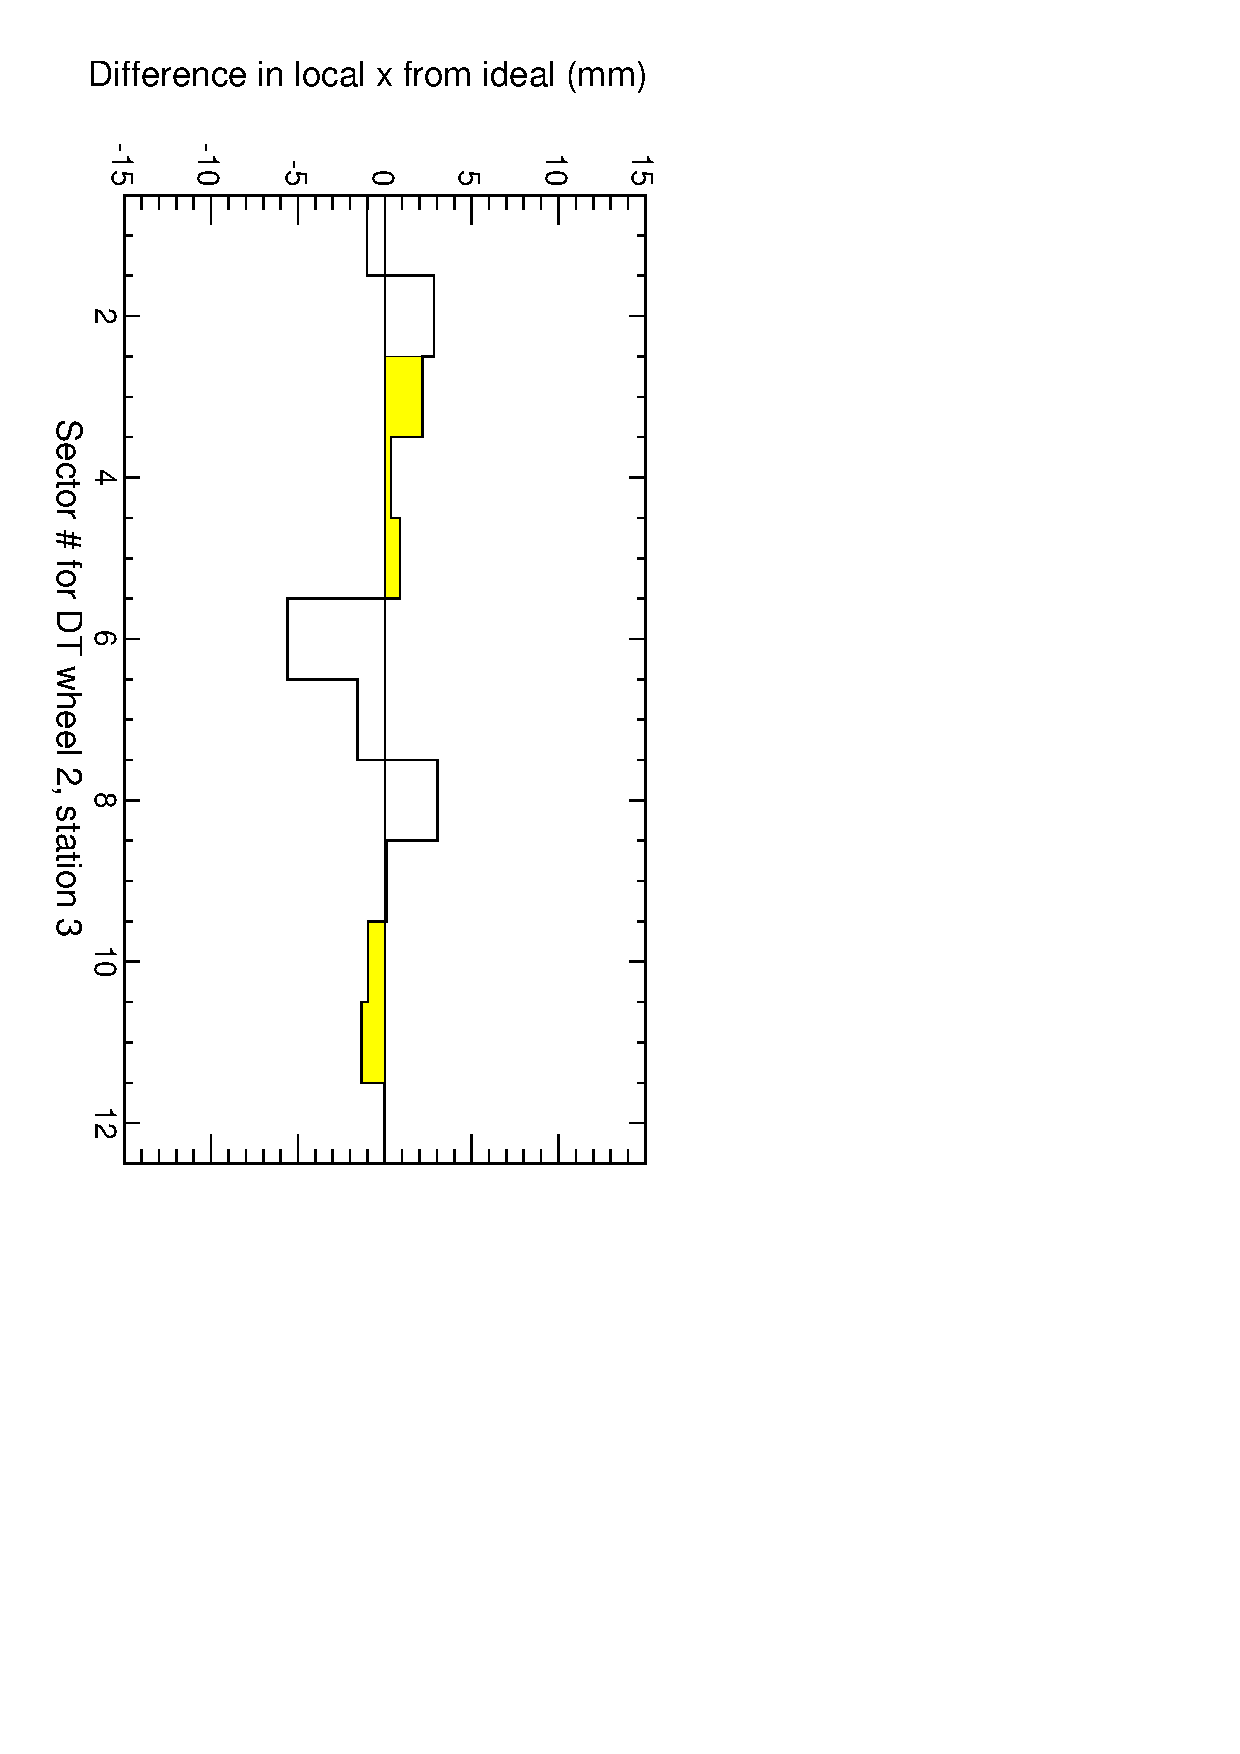
\includegraphics[height=0.5\linewidth, angle=90]{DThist014.pdf} 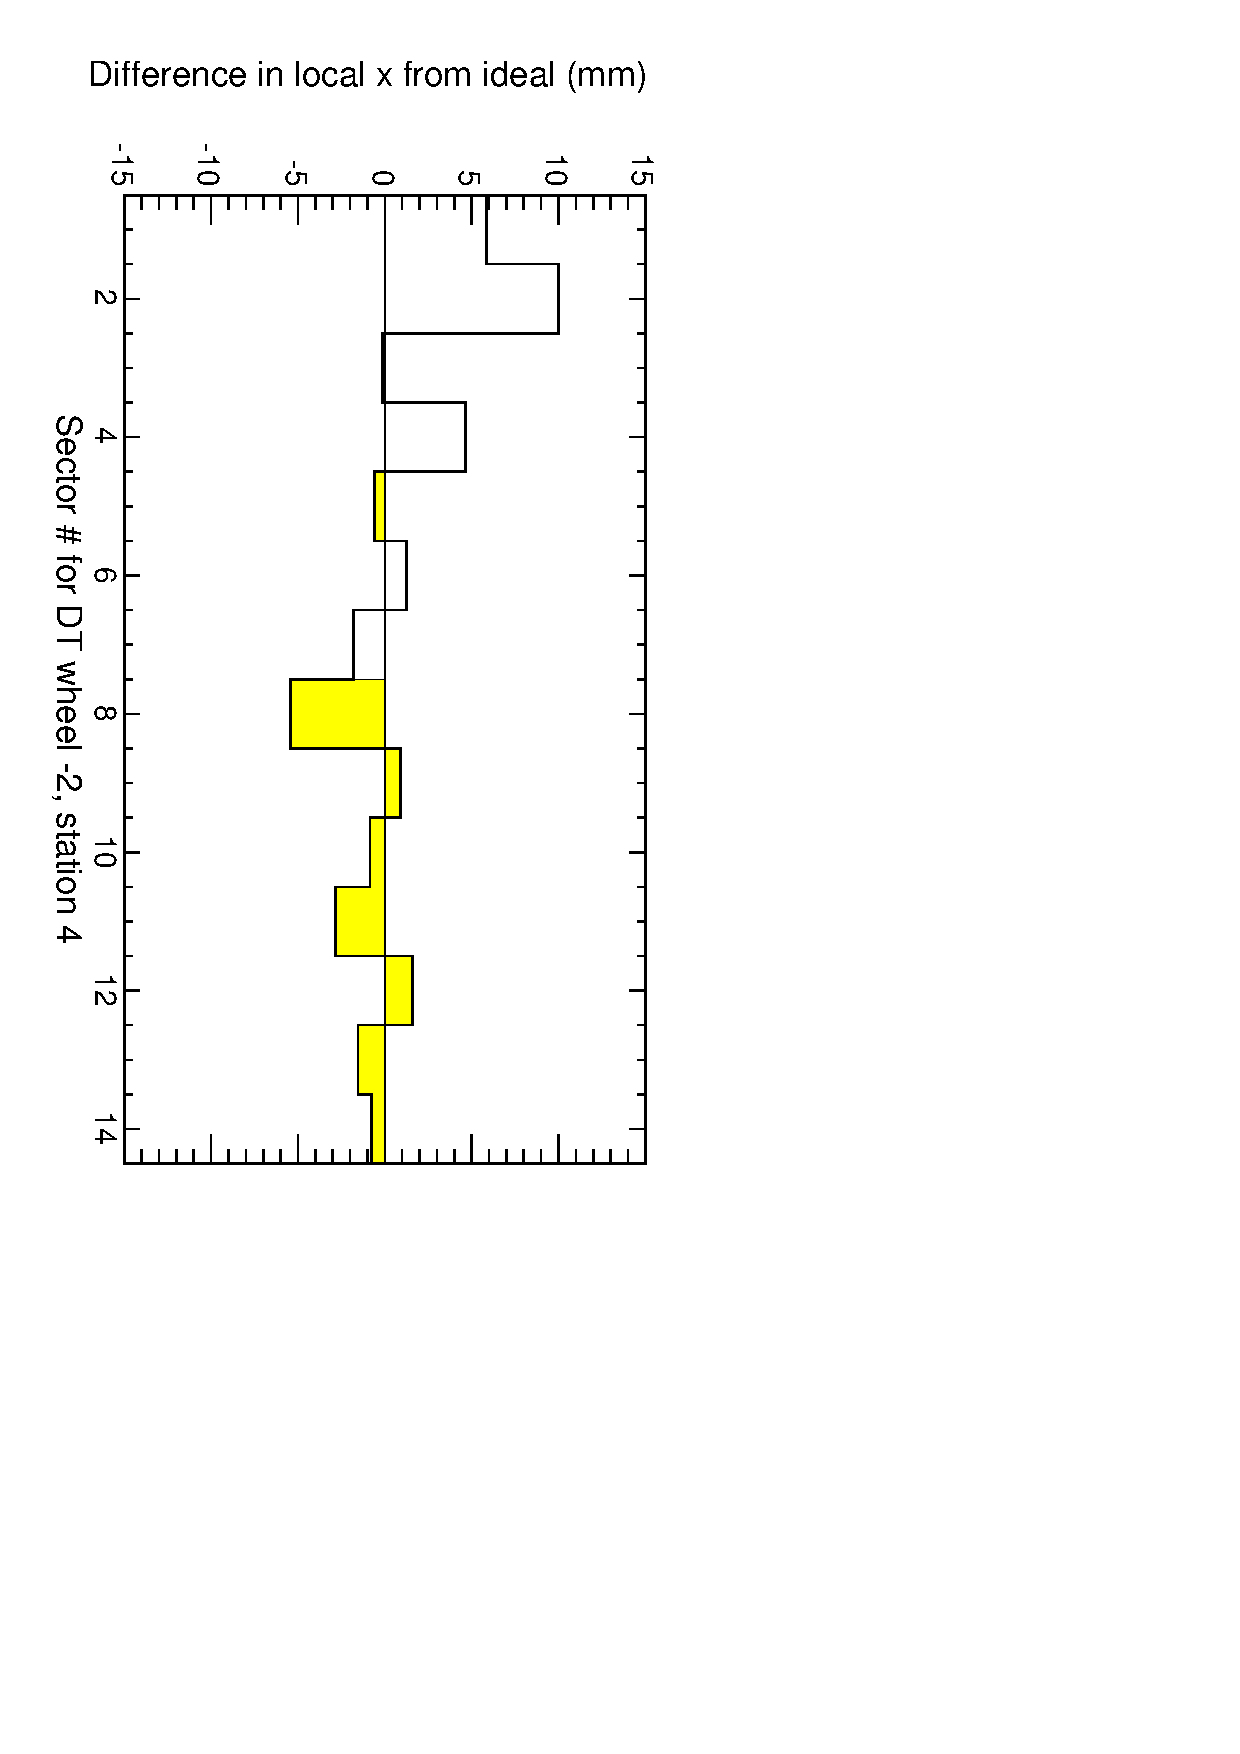
\includegraphics[height=0.5\linewidth, angle=90]{DThist015.pdf}
\end{frame}

\begin{frame}
\frametitle{Reference: all the constants}
\framesubtitle{Yellow denotes a parameter that was aligned with globalMuons}
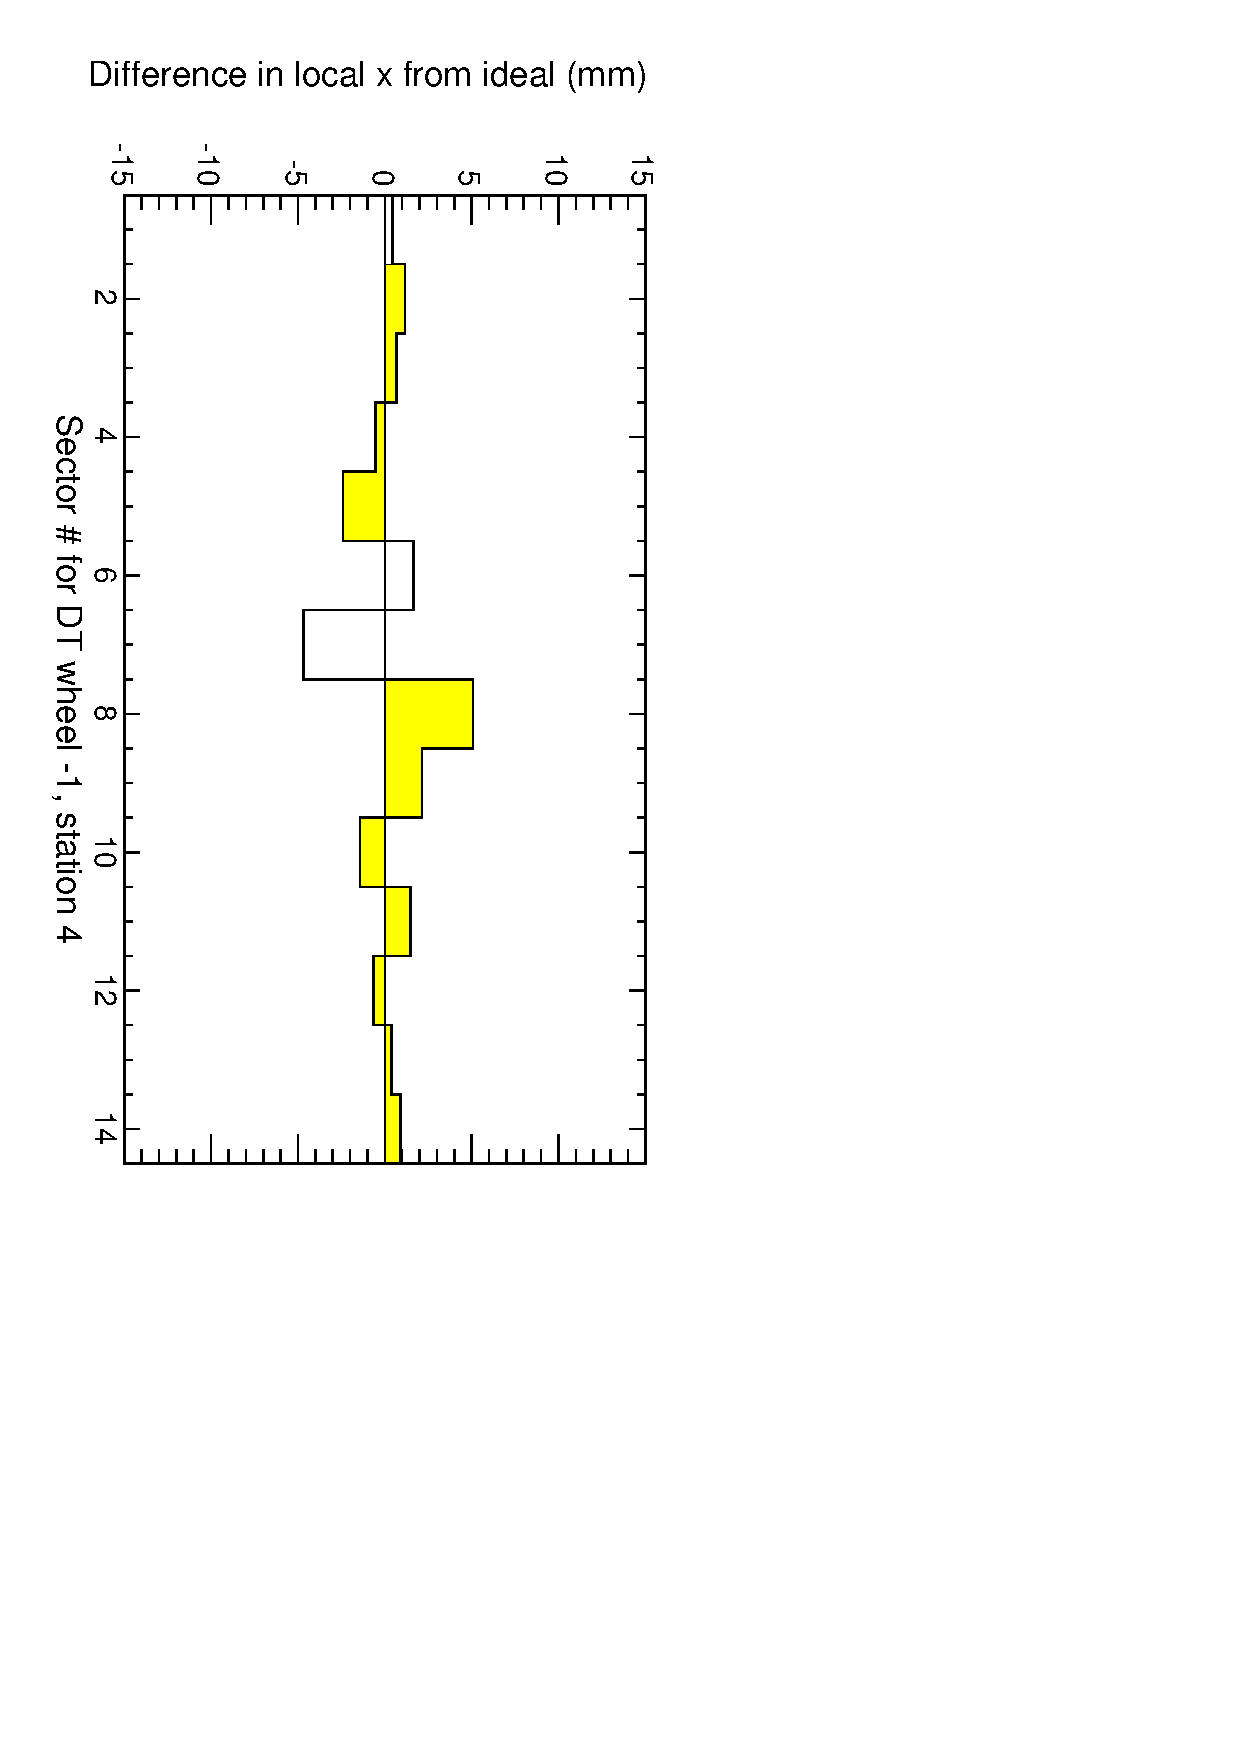
\includegraphics[height=0.5\linewidth, angle=90]{DThist016.pdf} 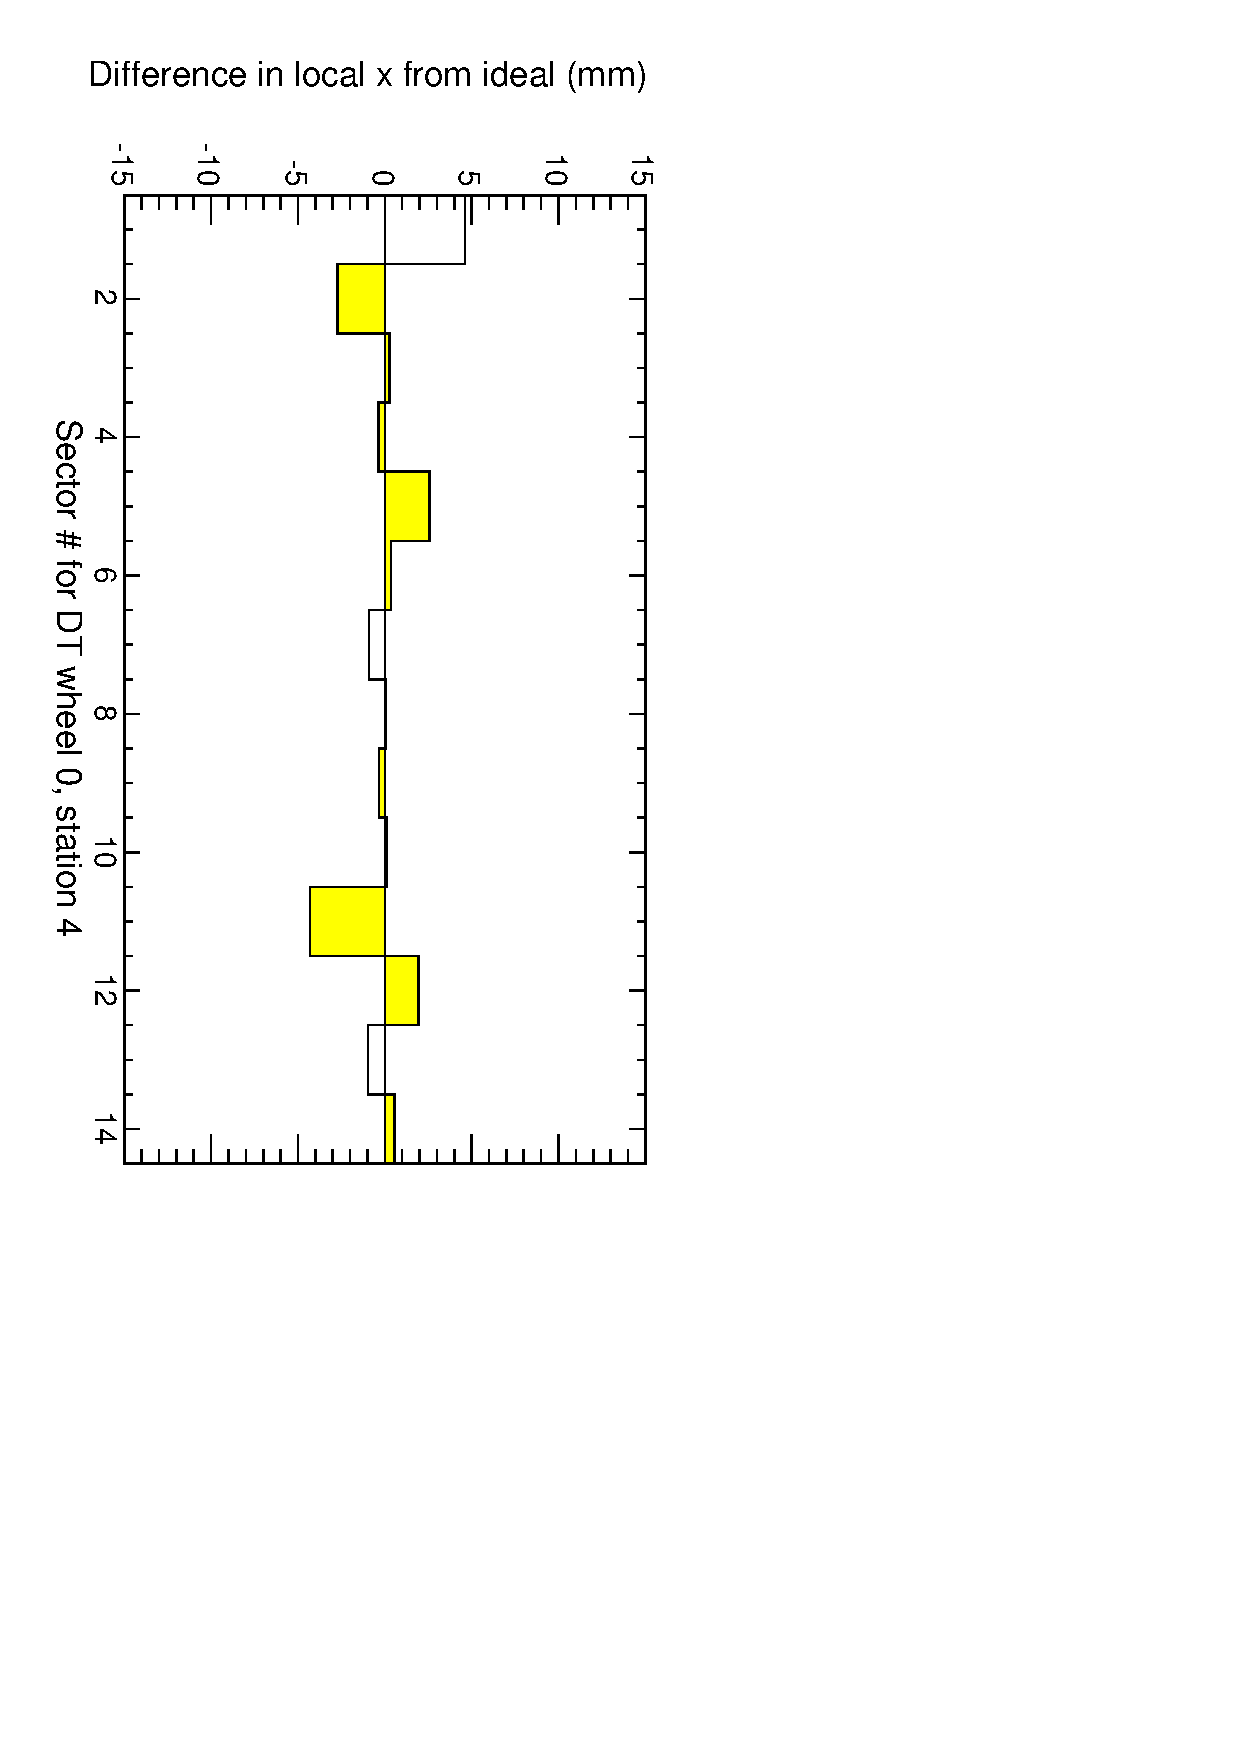
\includegraphics[height=0.5\linewidth, angle=90]{DThist017.pdf} \\
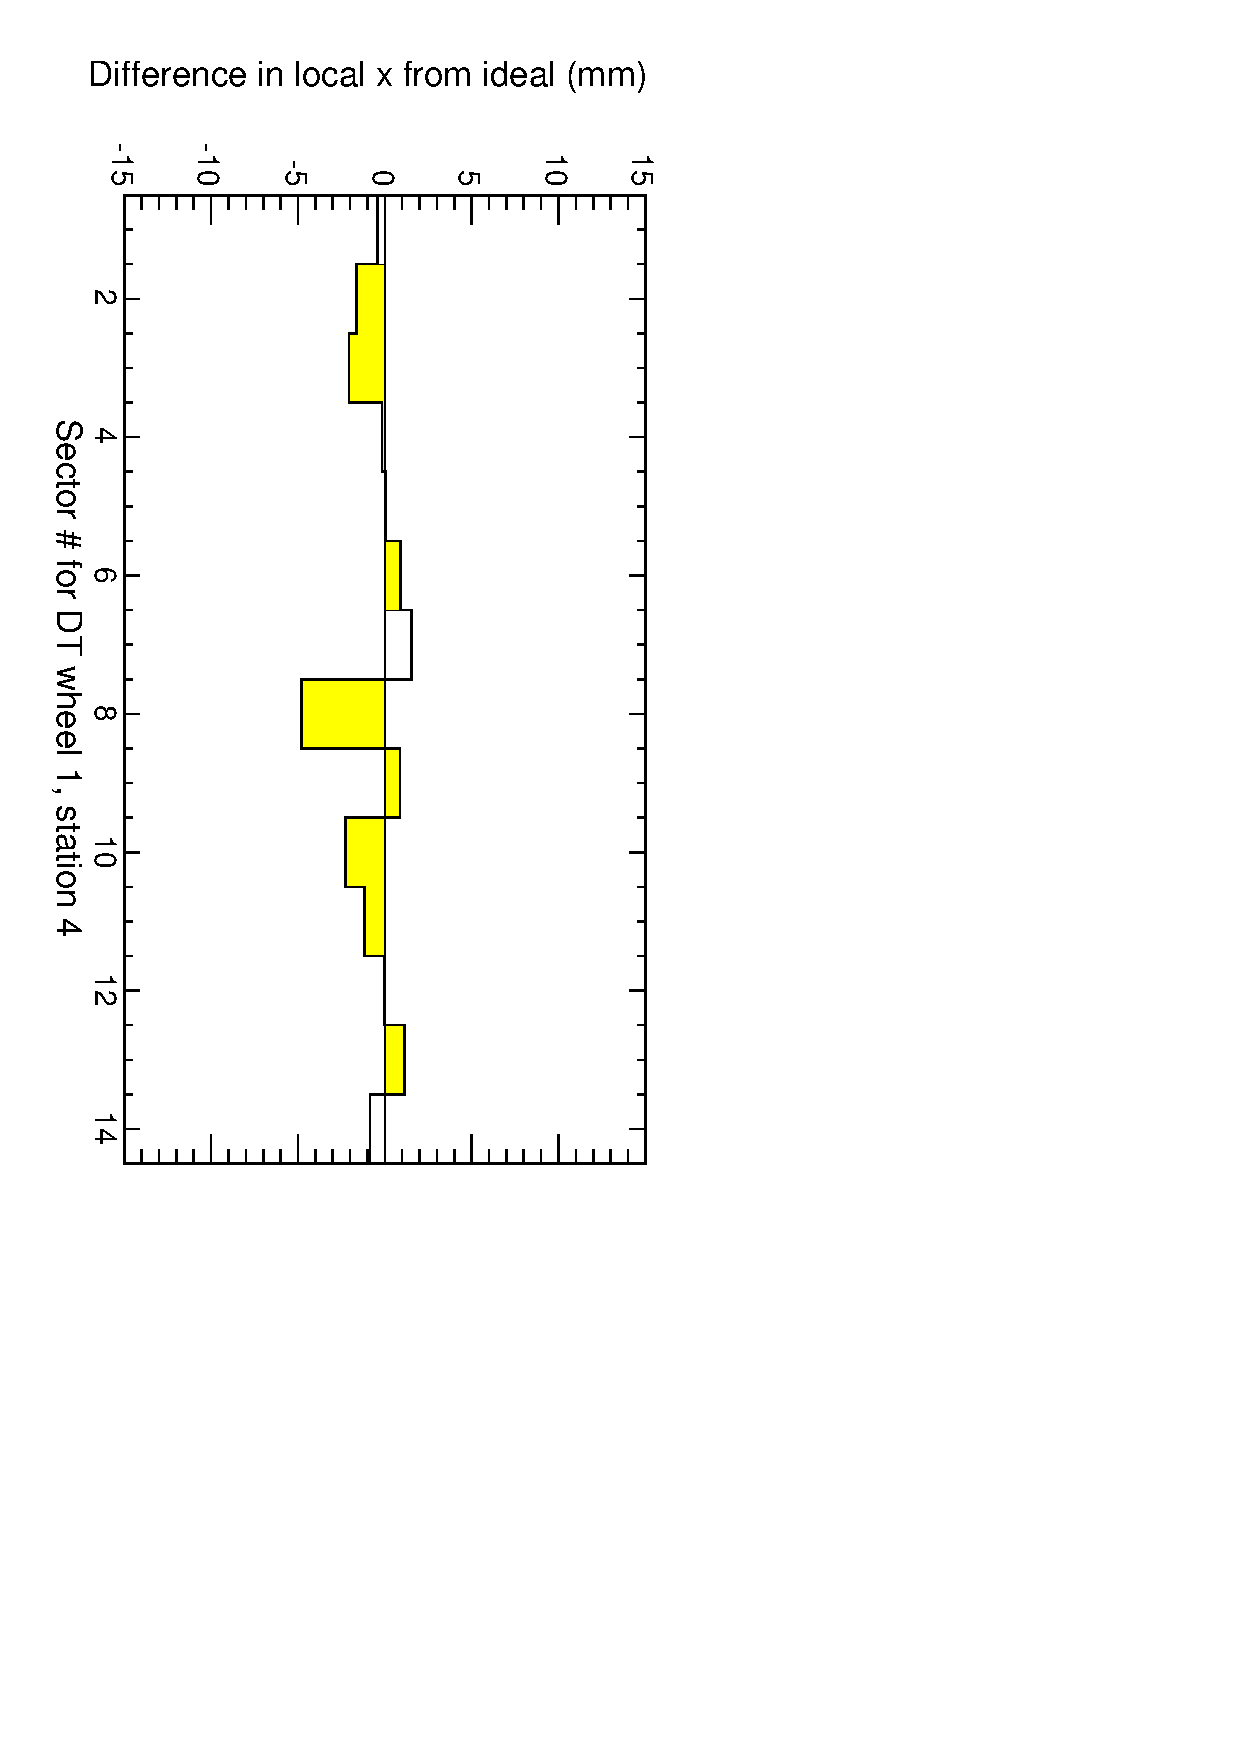
\includegraphics[height=0.5\linewidth, angle=90]{DThist018.pdf} 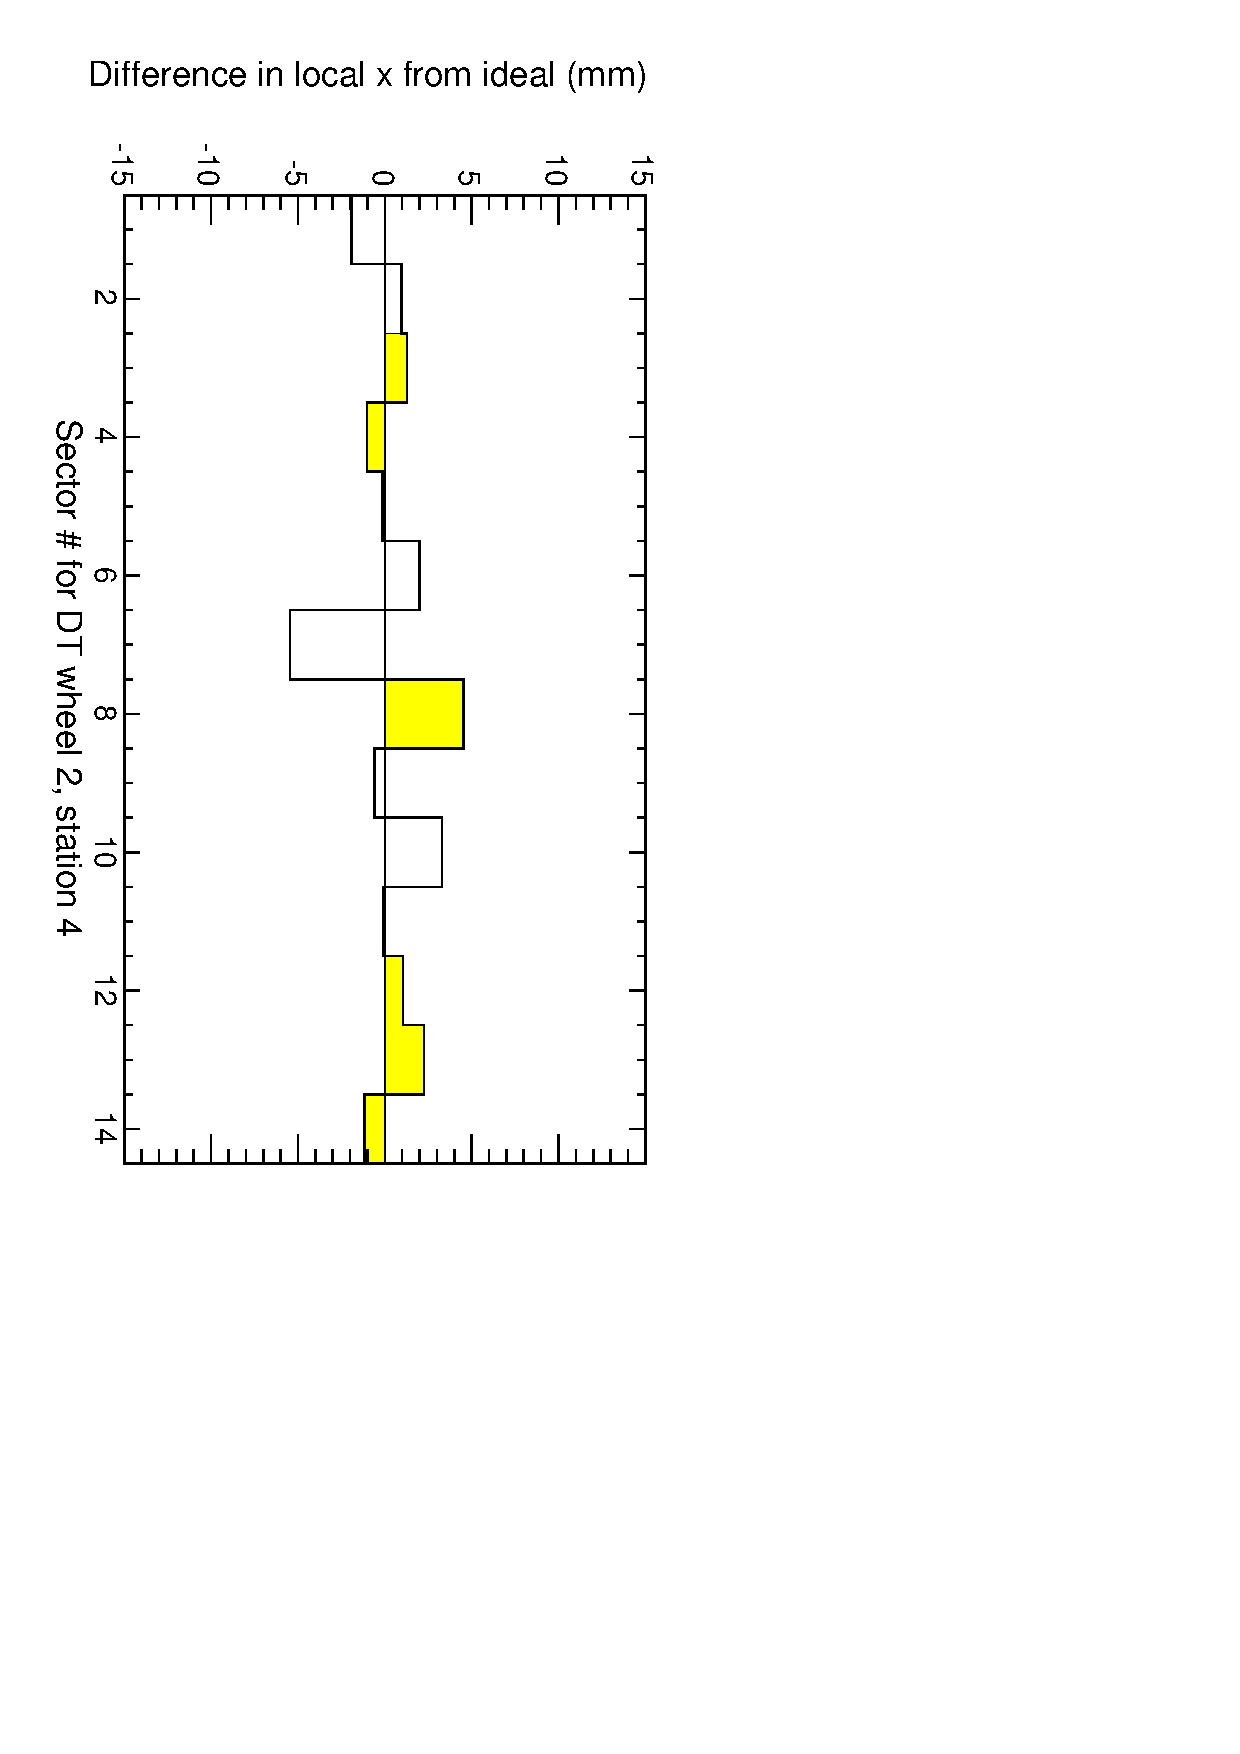
\includegraphics[height=0.5\linewidth, angle=90]{DThist019.pdf}
\end{frame}

\begin{frame}
\frametitle{Reference: all the constants}
\framesubtitle{Yellow denotes a parameter that was aligned with globalMuons}
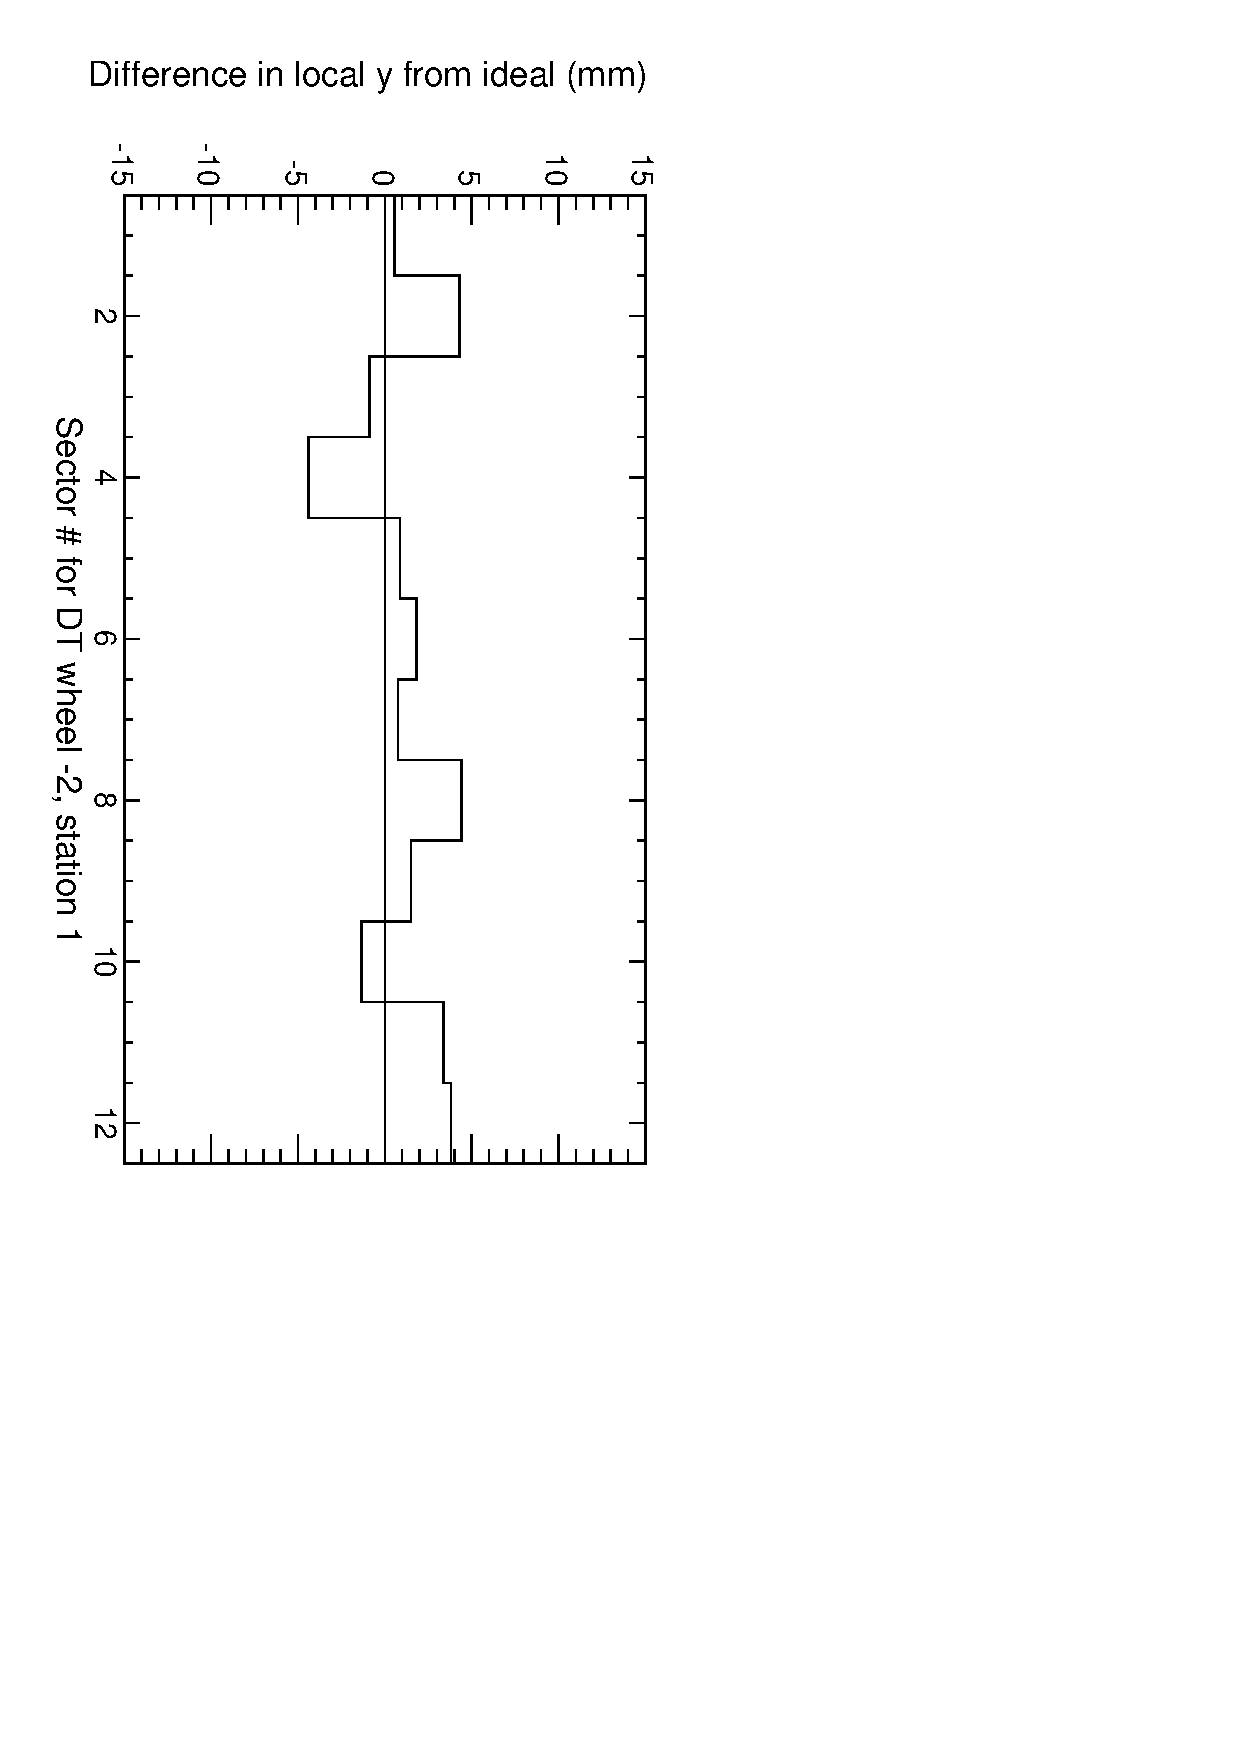
\includegraphics[height=0.5\linewidth, angle=90]{DThist020.pdf} 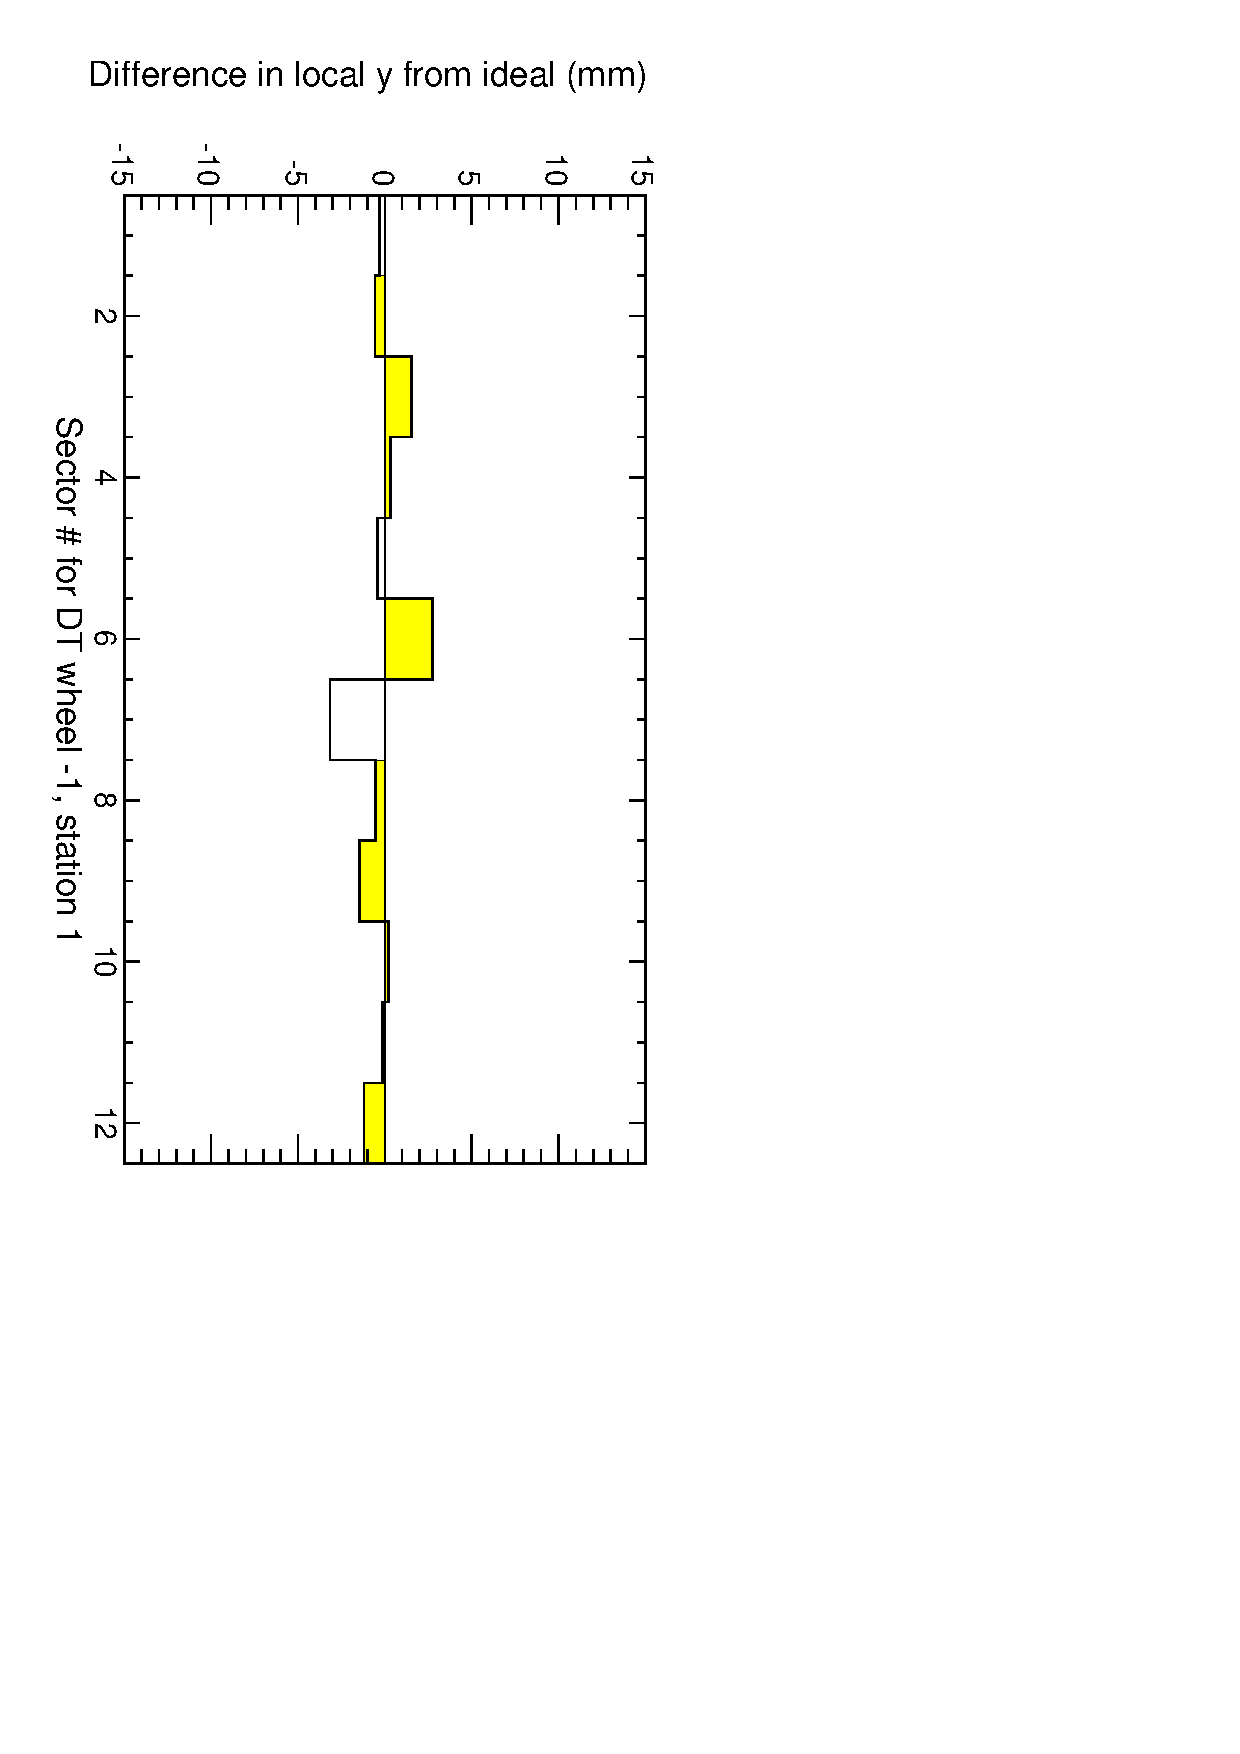
\includegraphics[height=0.5\linewidth, angle=90]{DThist021.pdf} \\
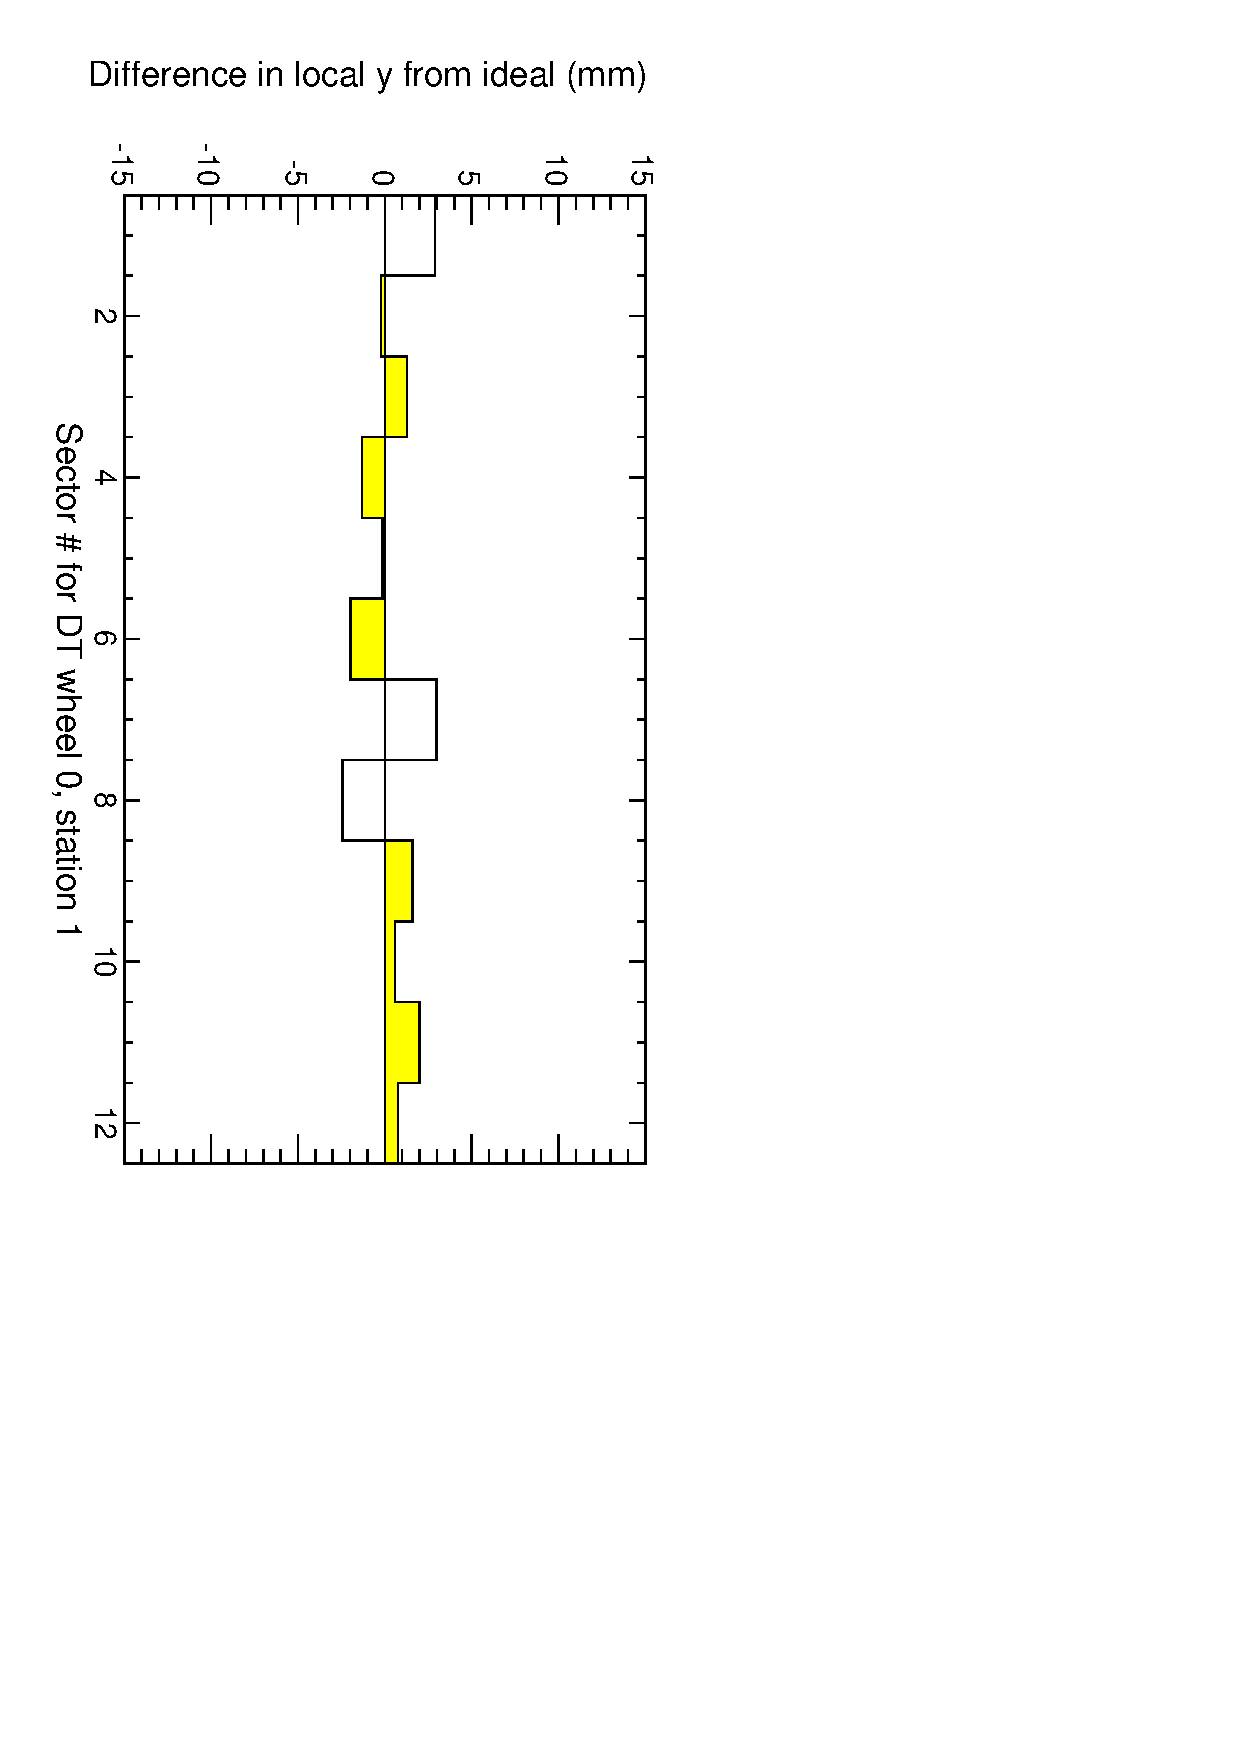
\includegraphics[height=0.5\linewidth, angle=90]{DThist022.pdf} 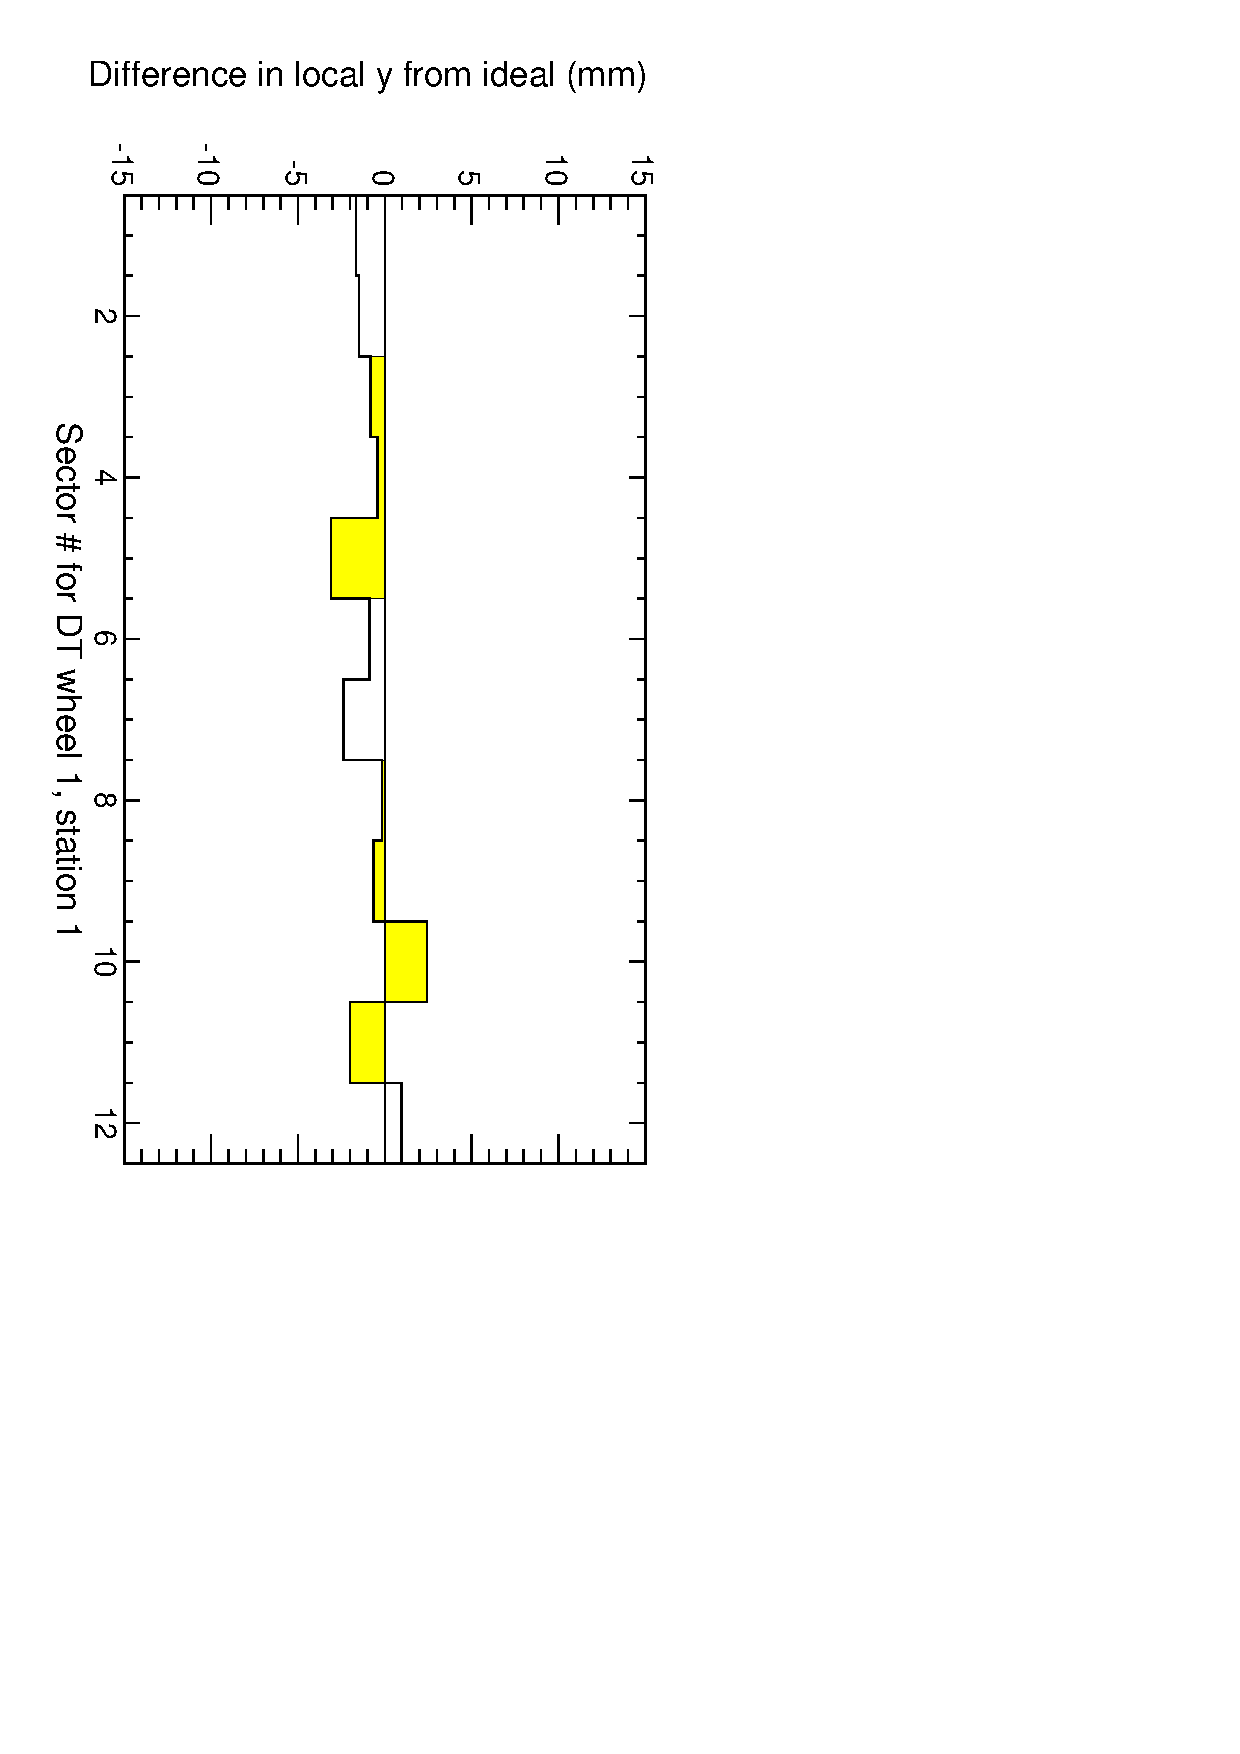
\includegraphics[height=0.5\linewidth, angle=90]{DThist023.pdf}
\end{frame}

\begin{frame}
\frametitle{Reference: all the constants}
\framesubtitle{Yellow denotes a parameter that was aligned with globalMuons}
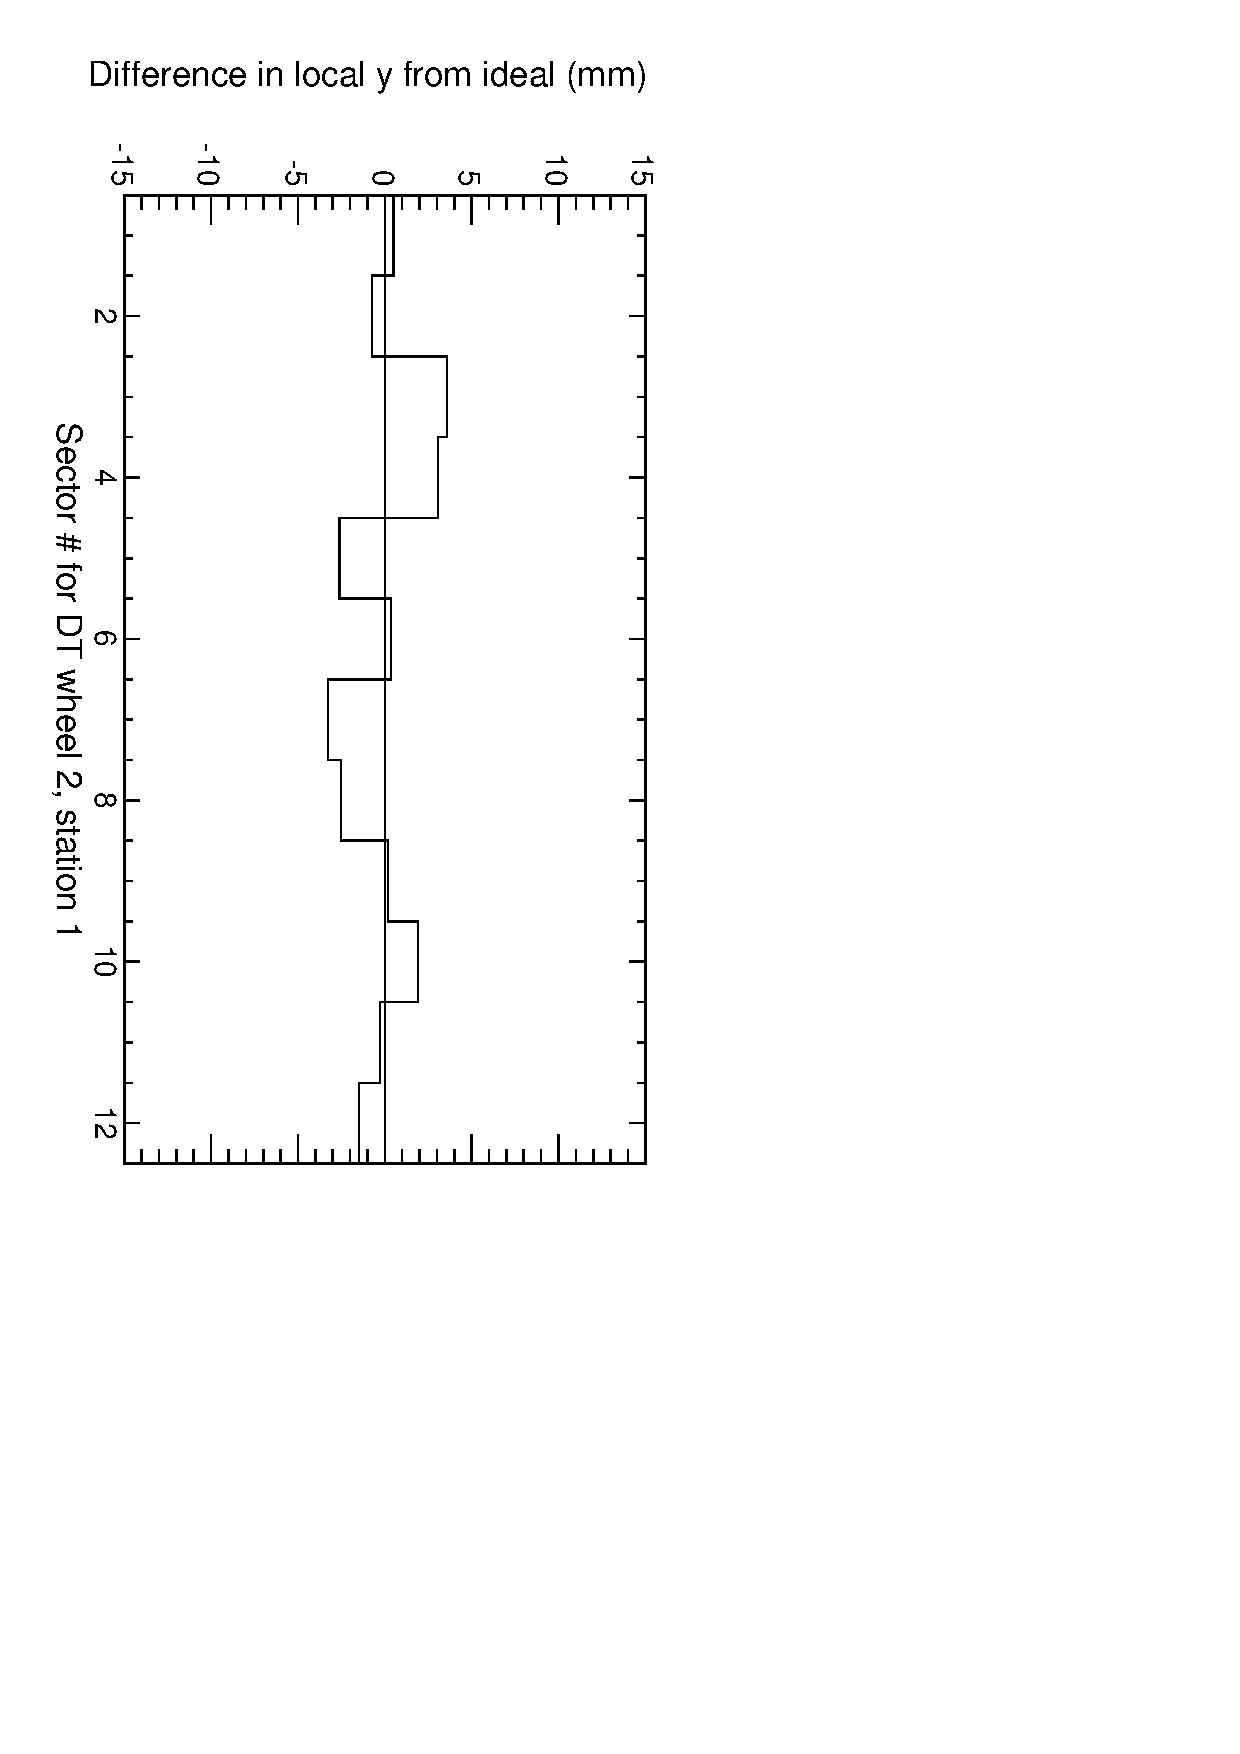
\includegraphics[height=0.5\linewidth, angle=90]{DThist024.pdf} 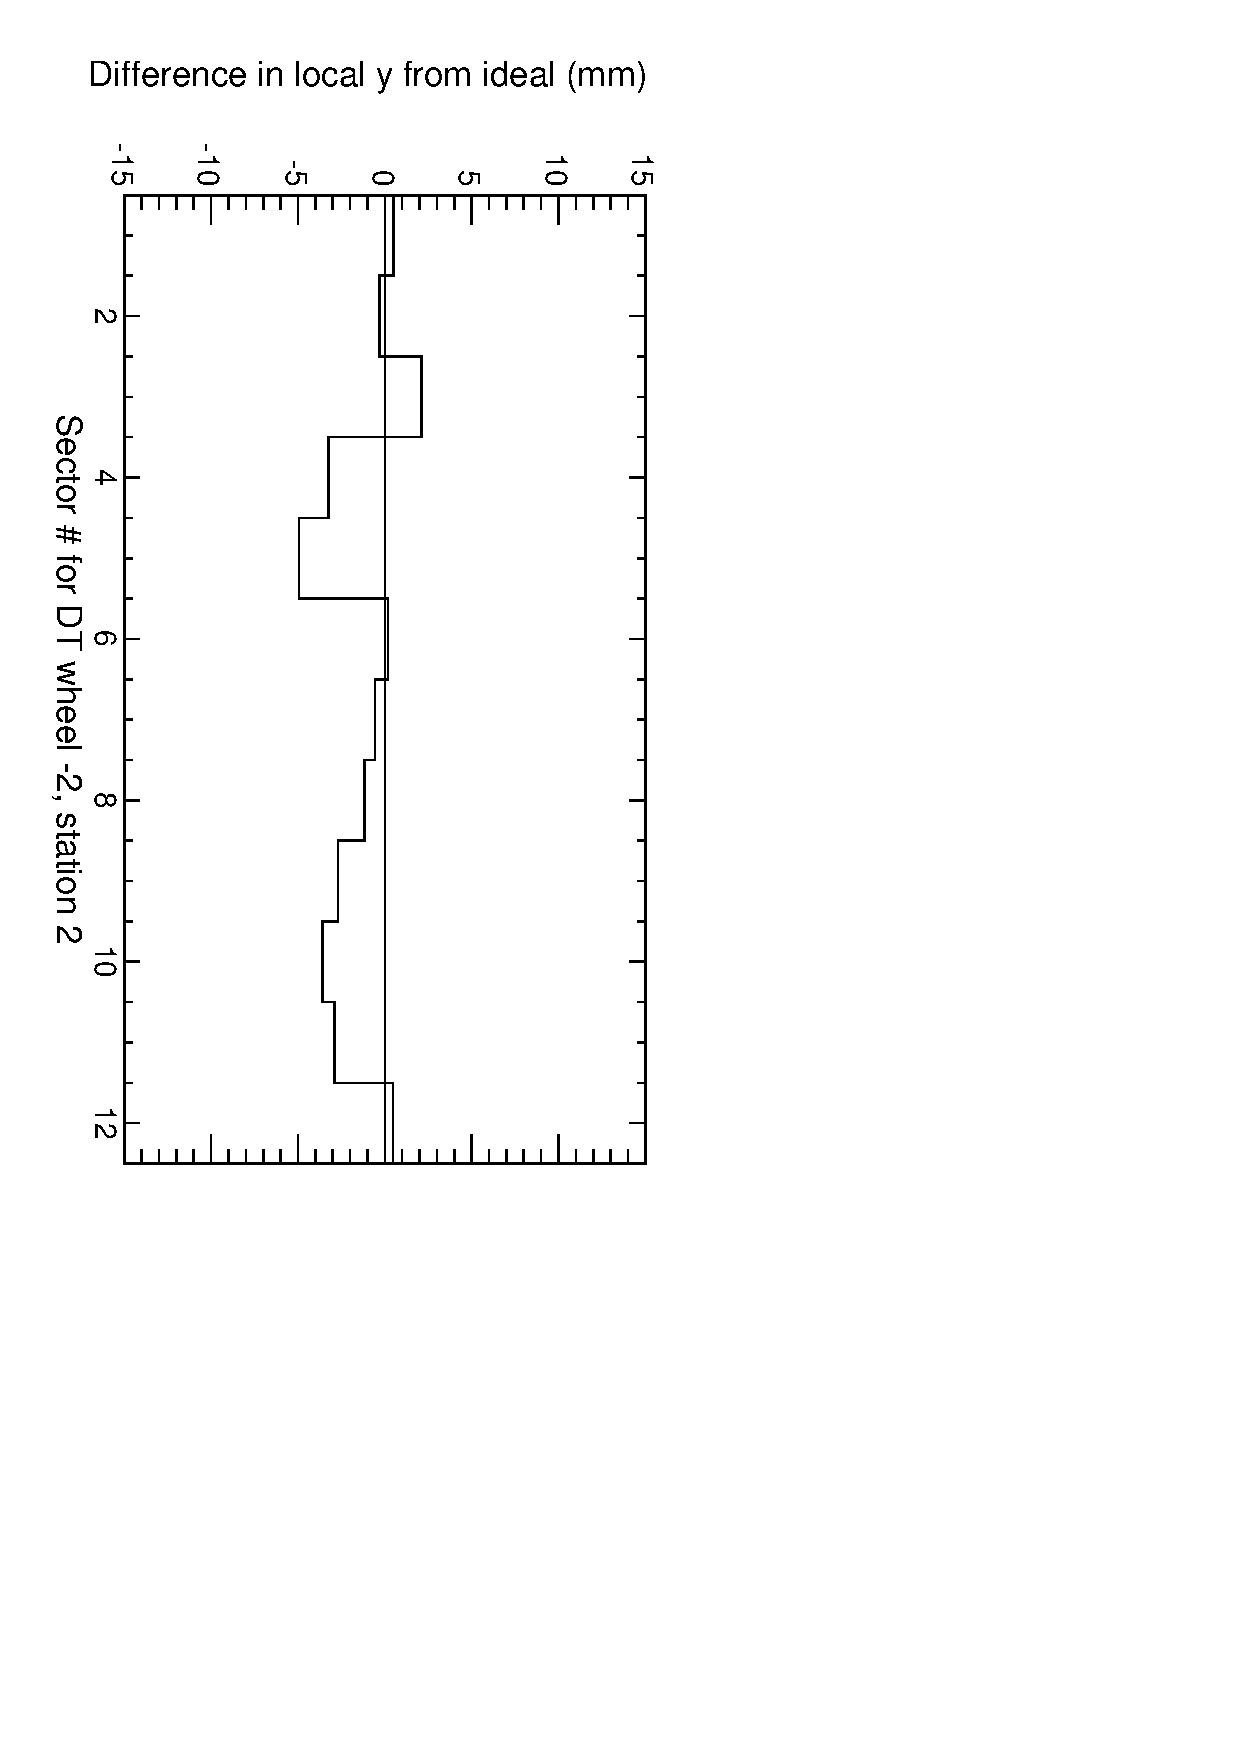
\includegraphics[height=0.5\linewidth, angle=90]{DThist025.pdf} \\
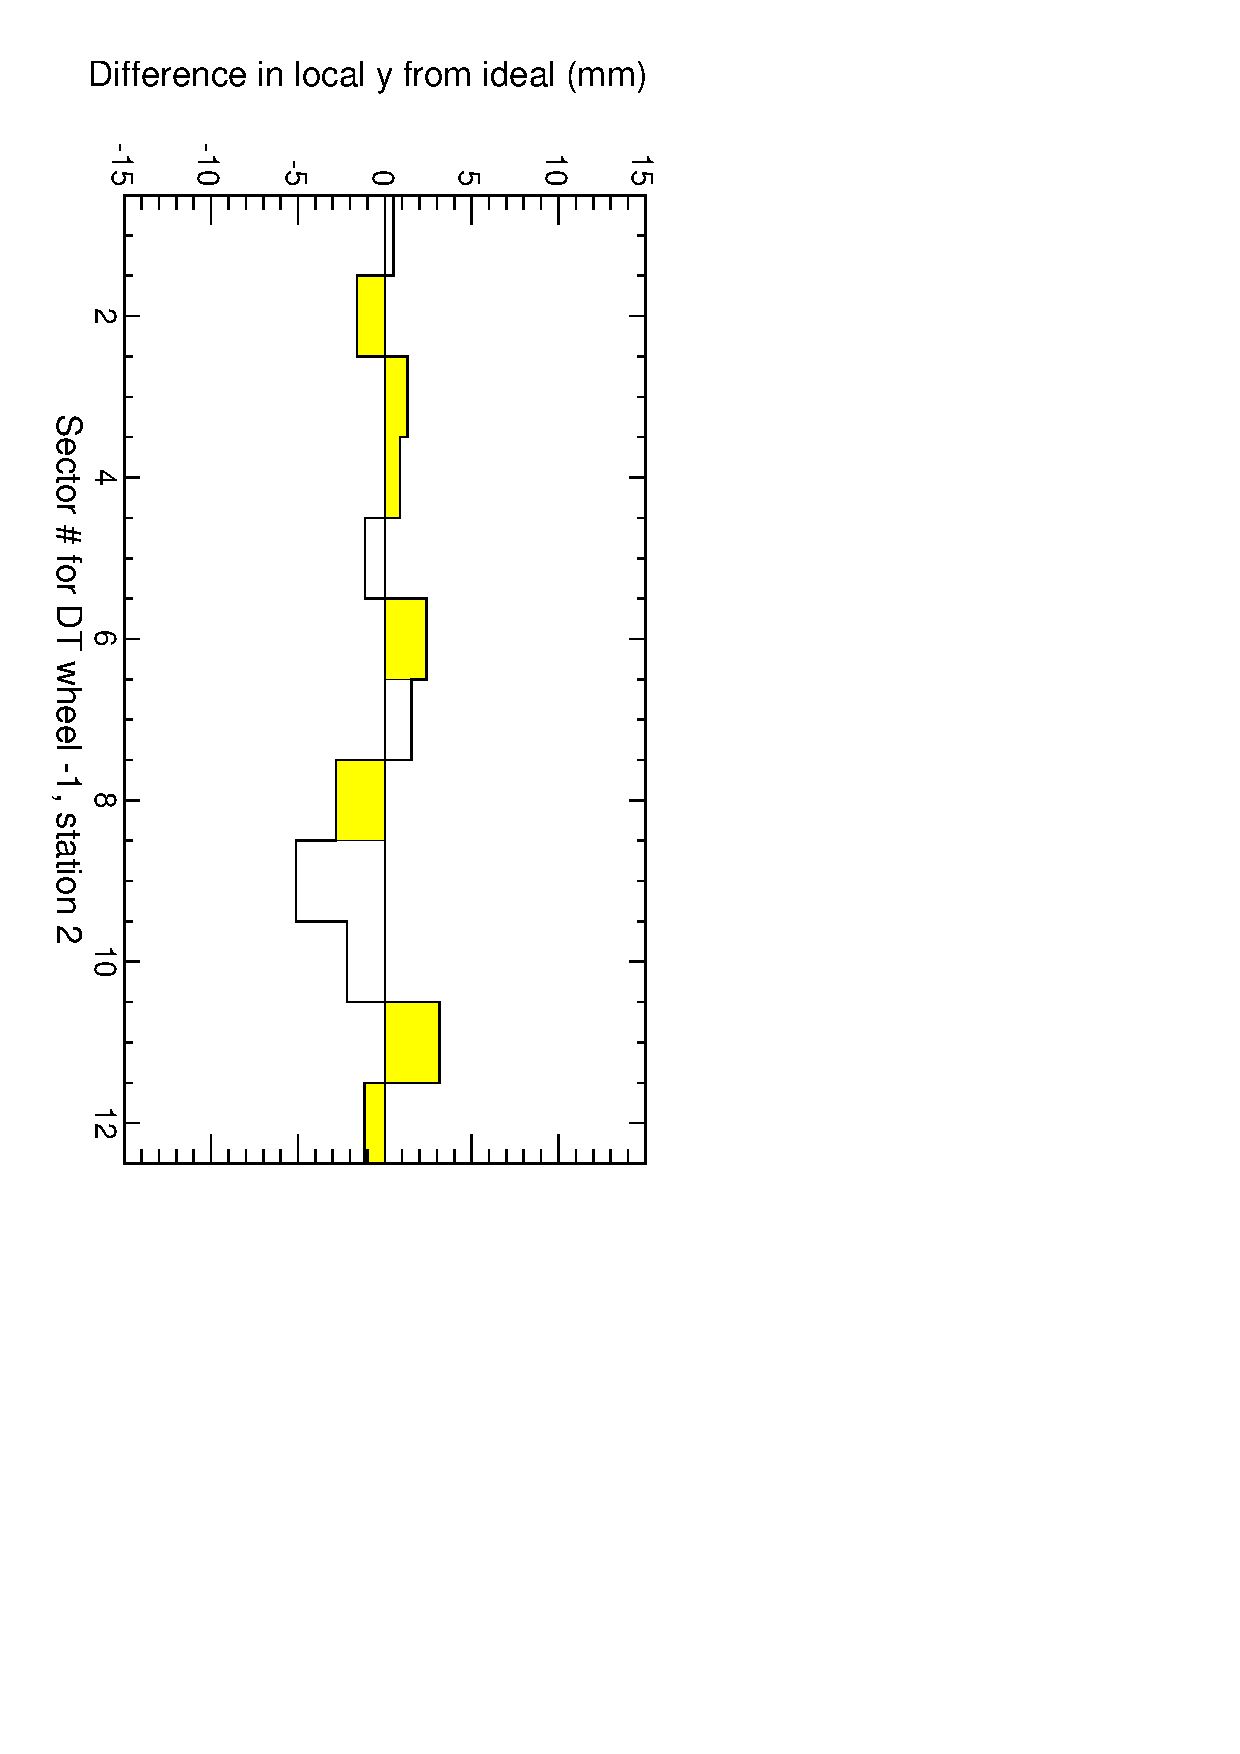
\includegraphics[height=0.5\linewidth, angle=90]{DThist026.pdf} 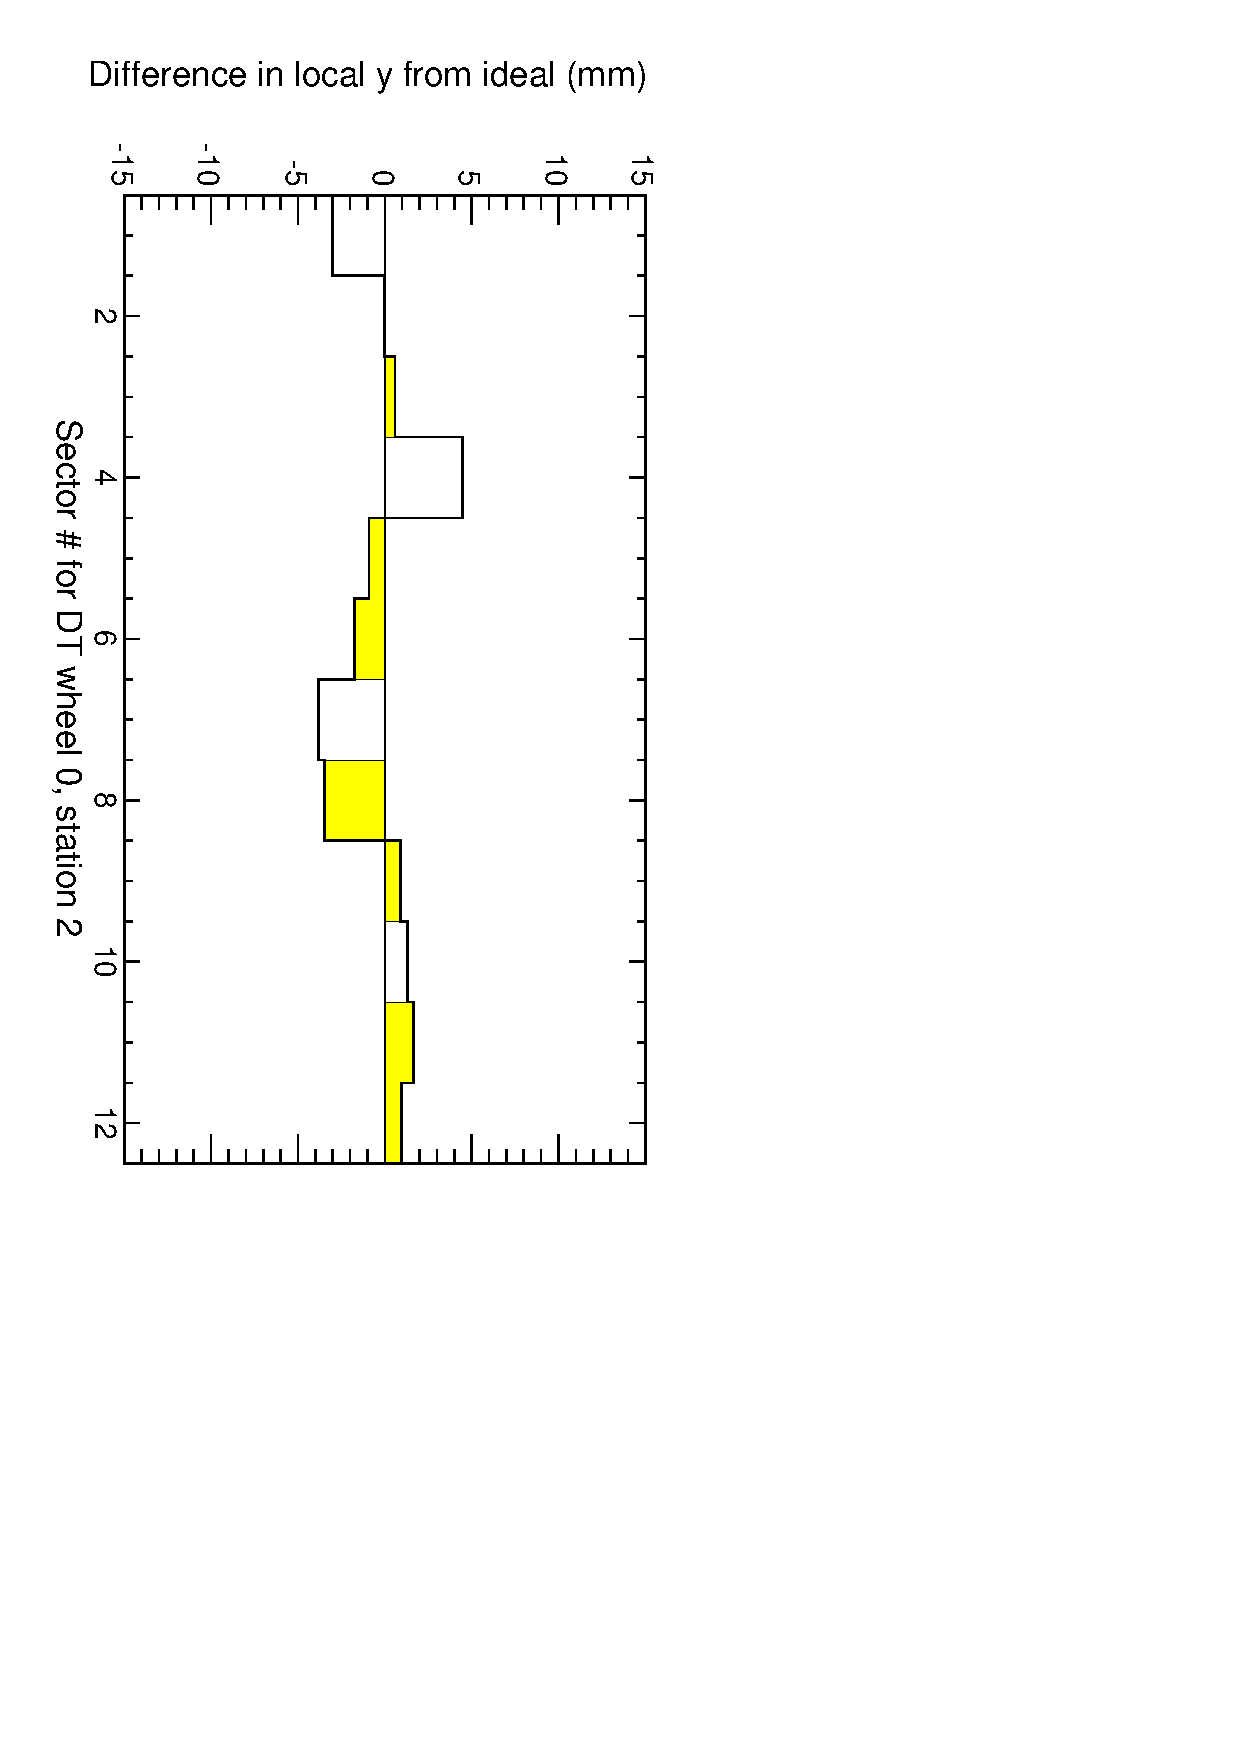
\includegraphics[height=0.5\linewidth, angle=90]{DThist027.pdf}
\end{frame}

\begin{frame}
\frametitle{Reference: all the constants}
\framesubtitle{Yellow denotes a parameter that was aligned with globalMuons}
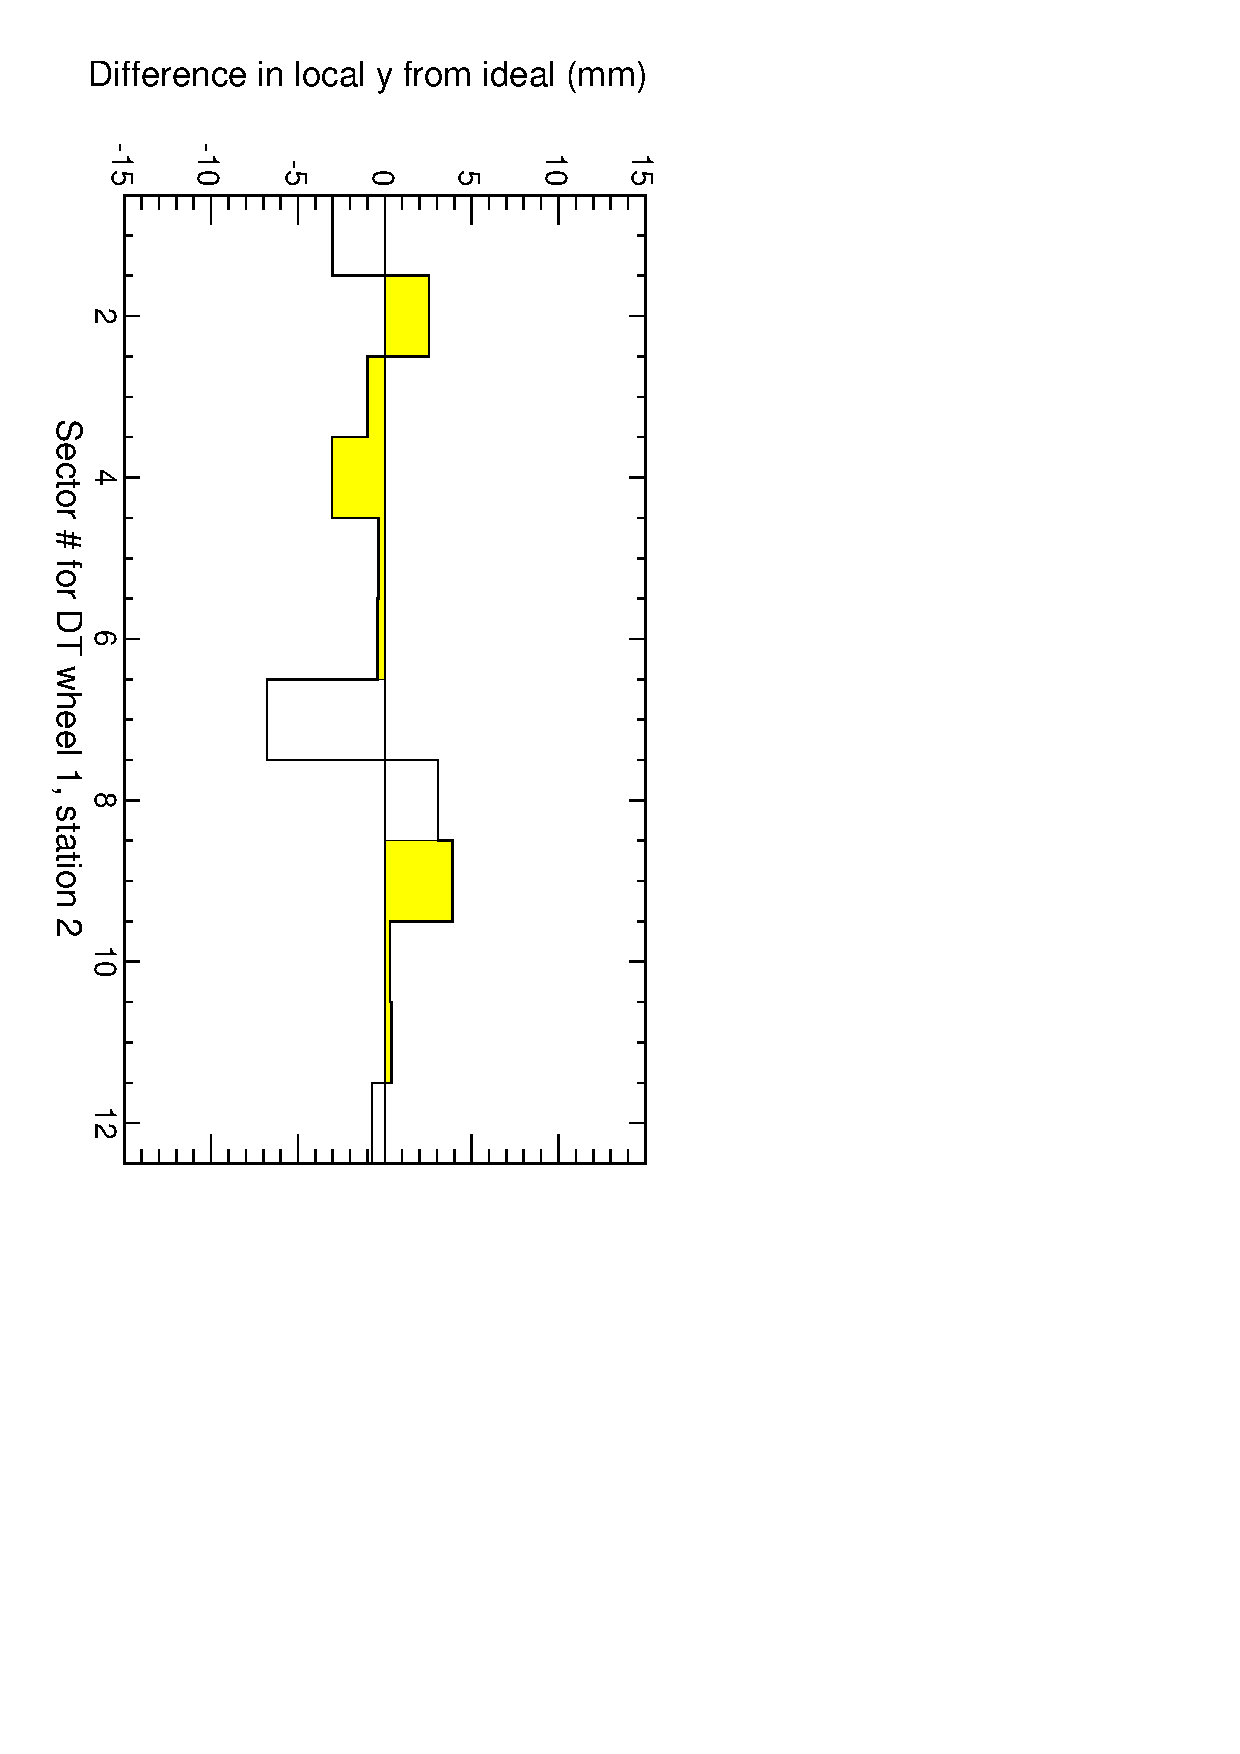
\includegraphics[height=0.5\linewidth, angle=90]{DThist028.pdf} 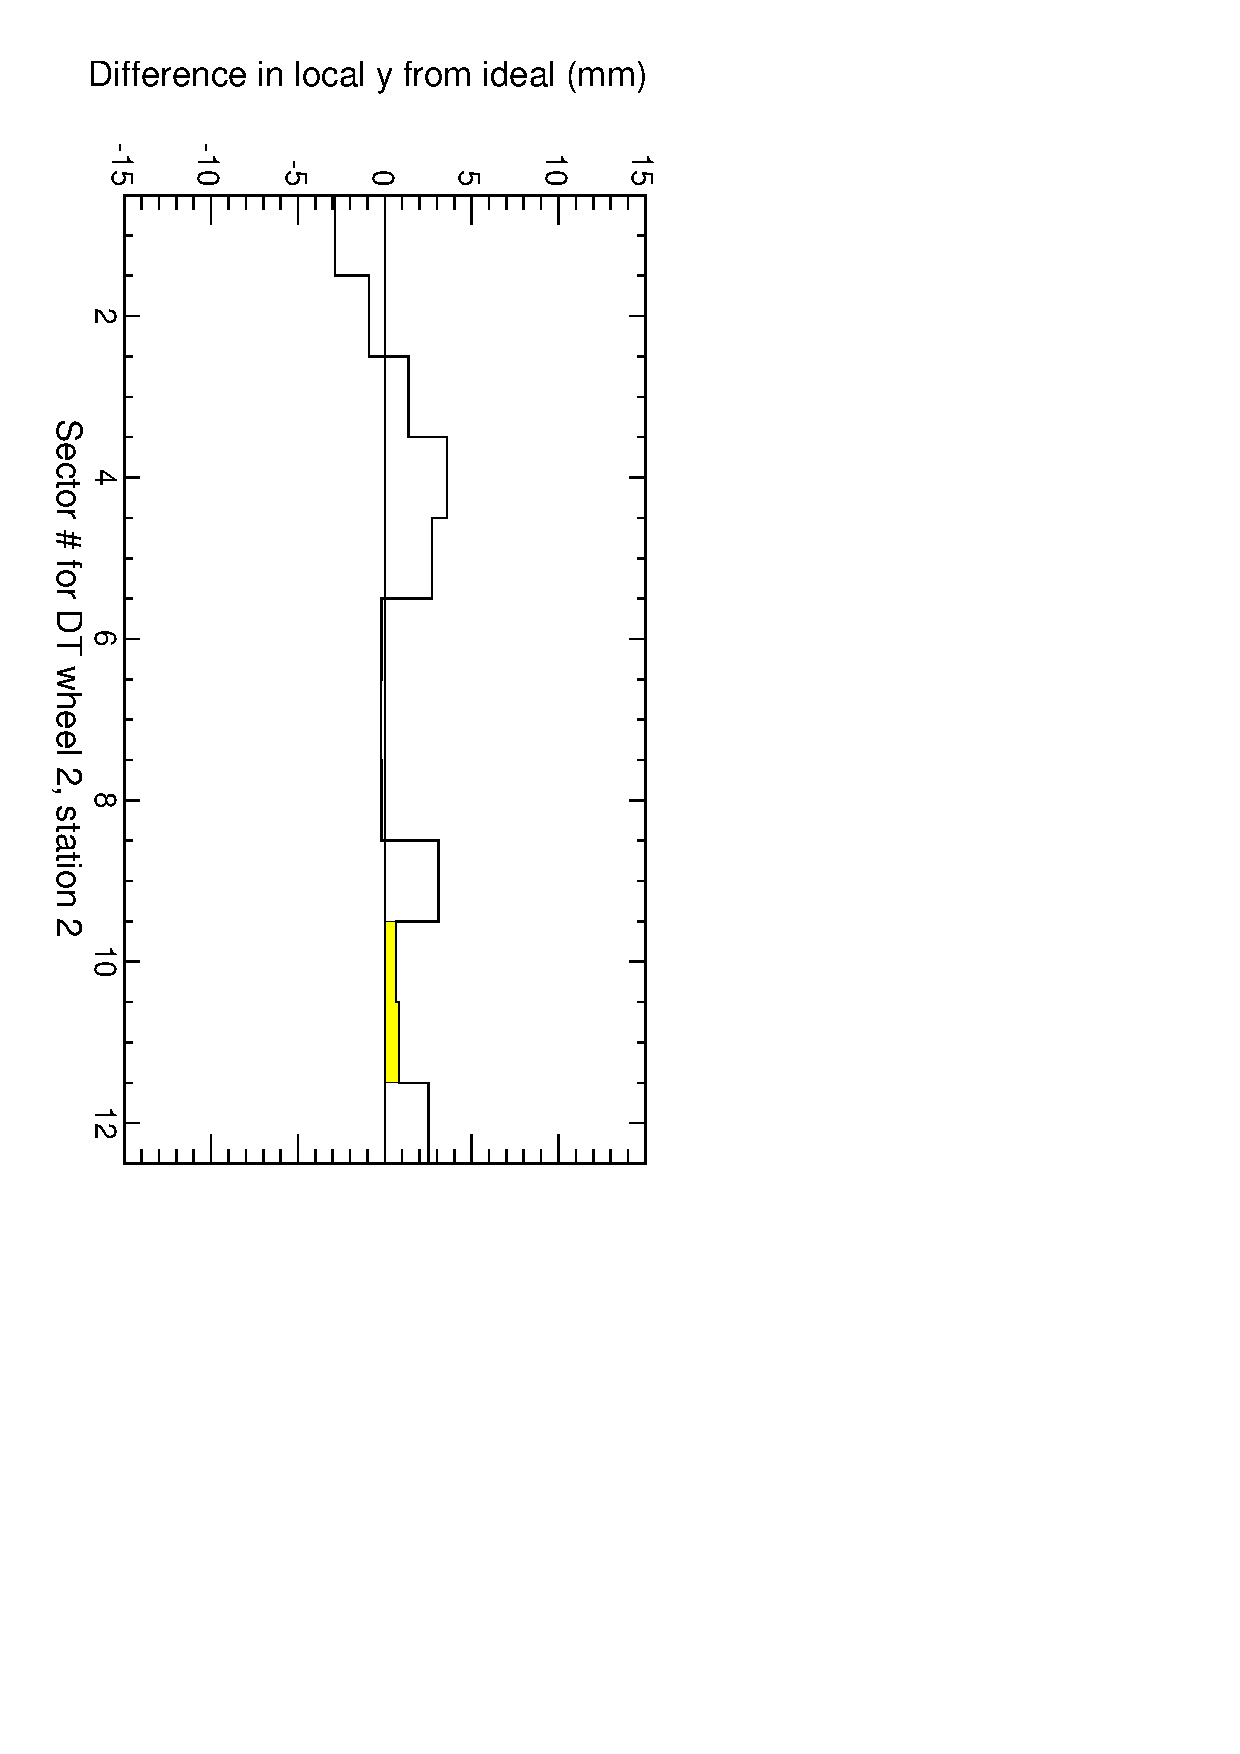
\includegraphics[height=0.5\linewidth, angle=90]{DThist029.pdf} \\
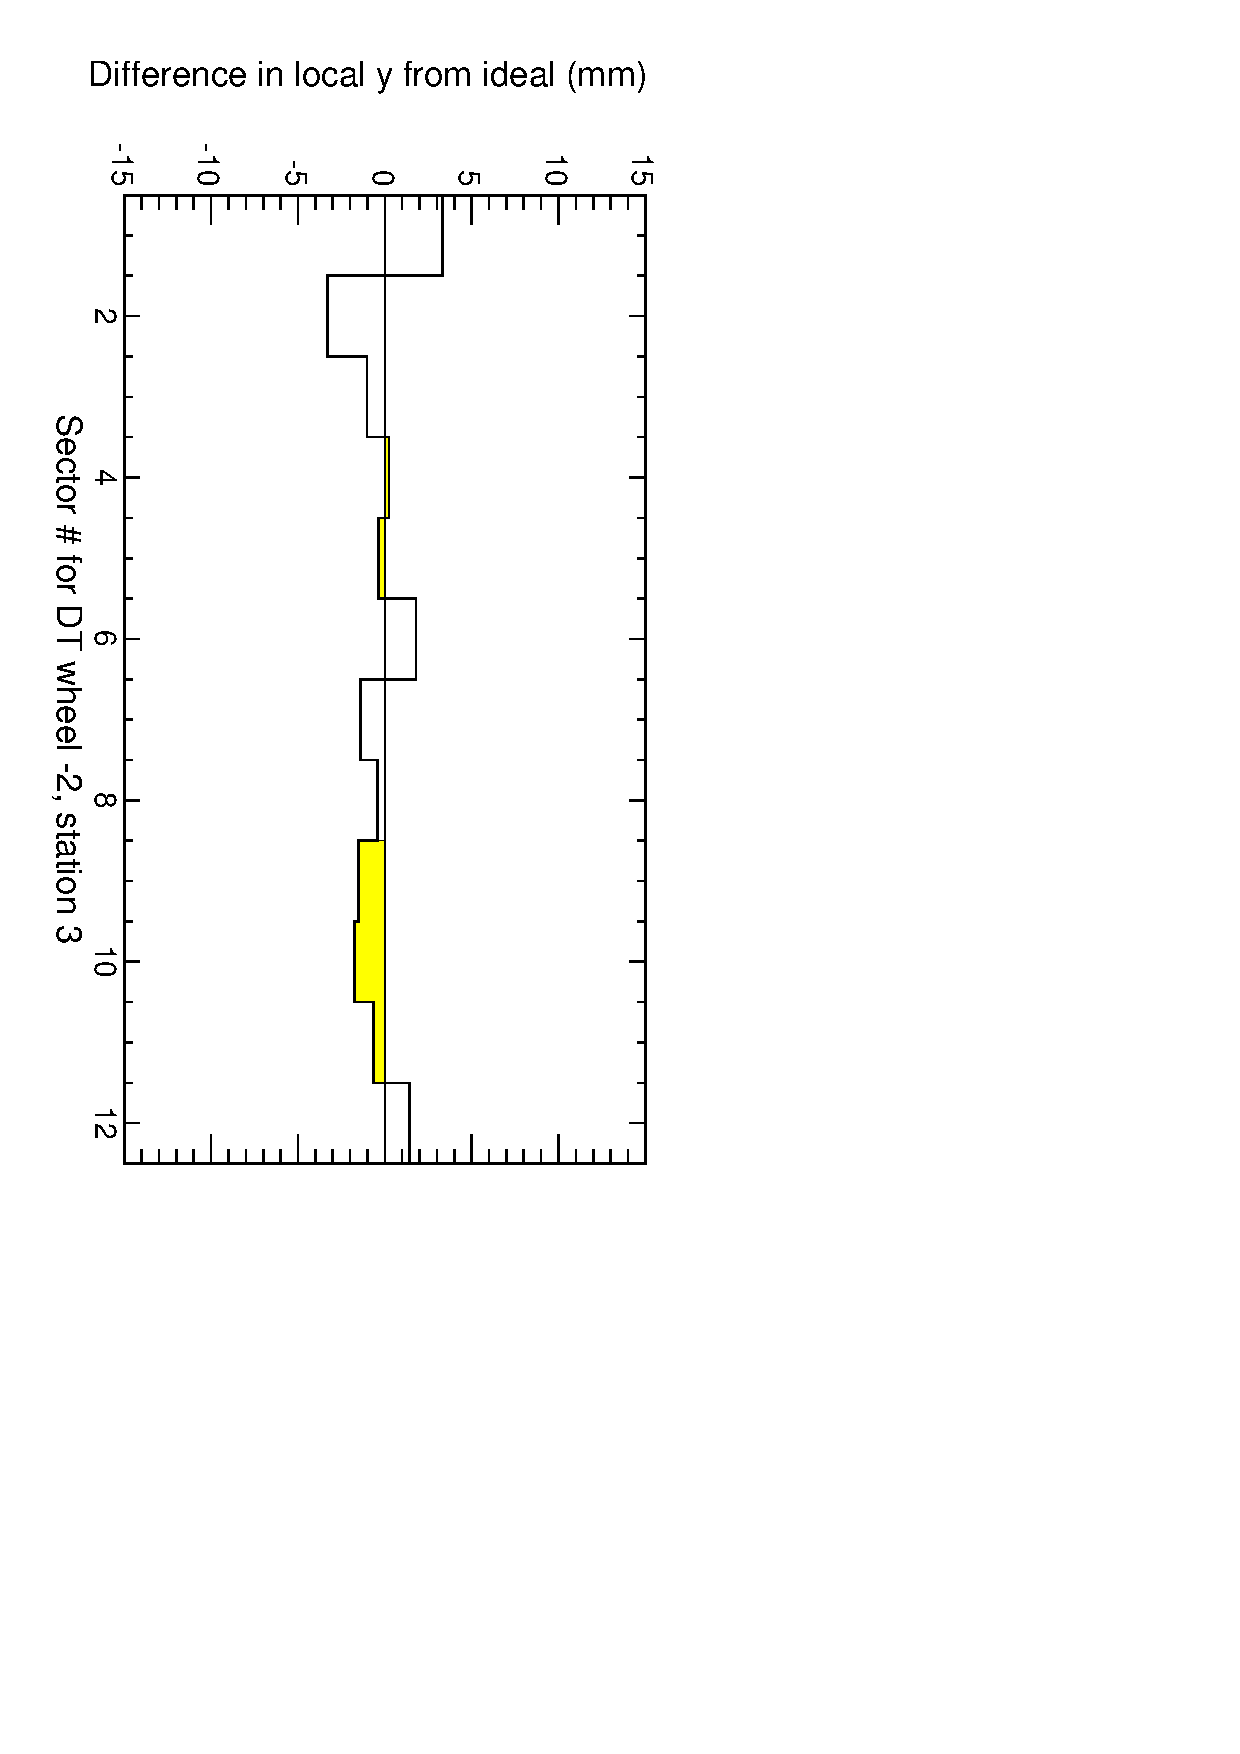
\includegraphics[height=0.5\linewidth, angle=90]{DThist030.pdf} 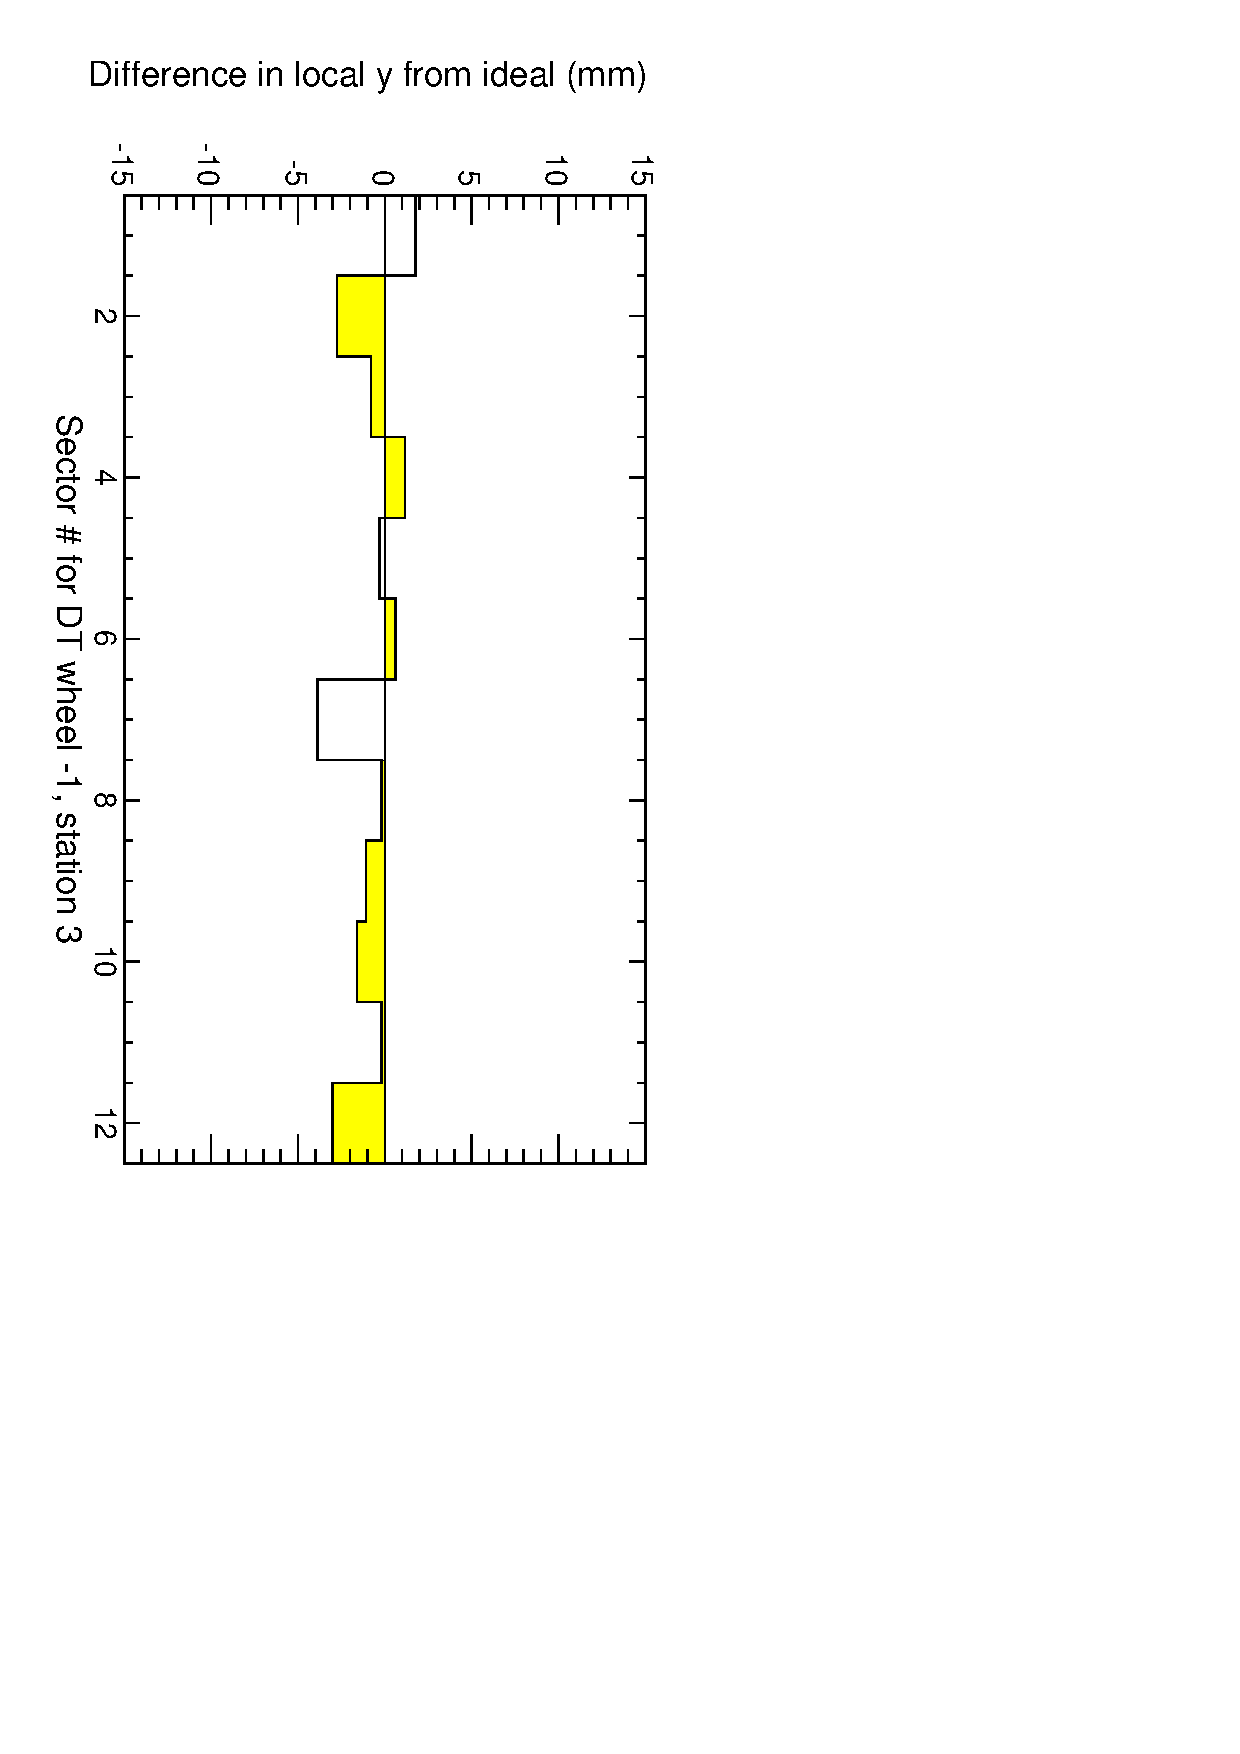
\includegraphics[height=0.5\linewidth, angle=90]{DThist031.pdf}
\end{frame}

\begin{frame}
\frametitle{Reference: all the constants}
\framesubtitle{Yellow denotes a parameter that was aligned with globalMuons}
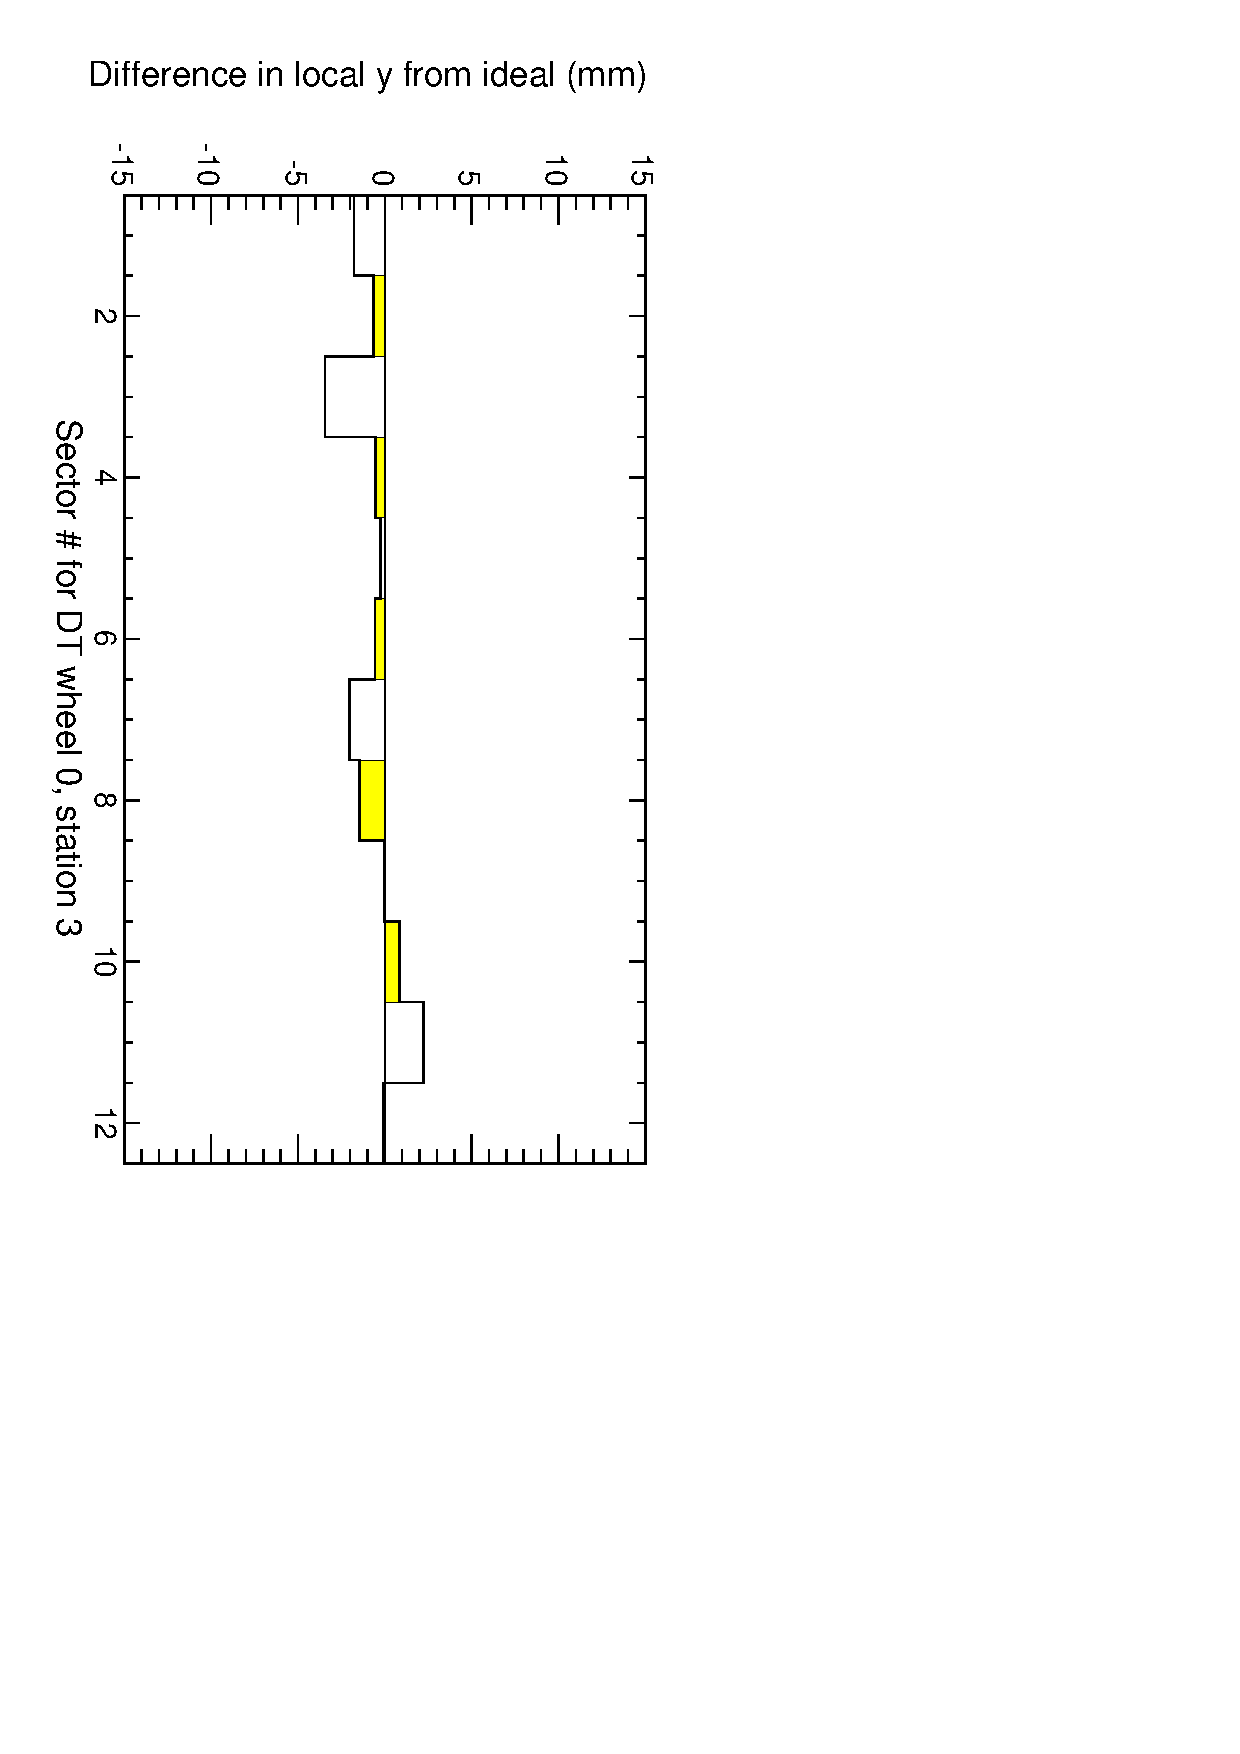
\includegraphics[height=0.5\linewidth, angle=90]{DThist032.pdf} 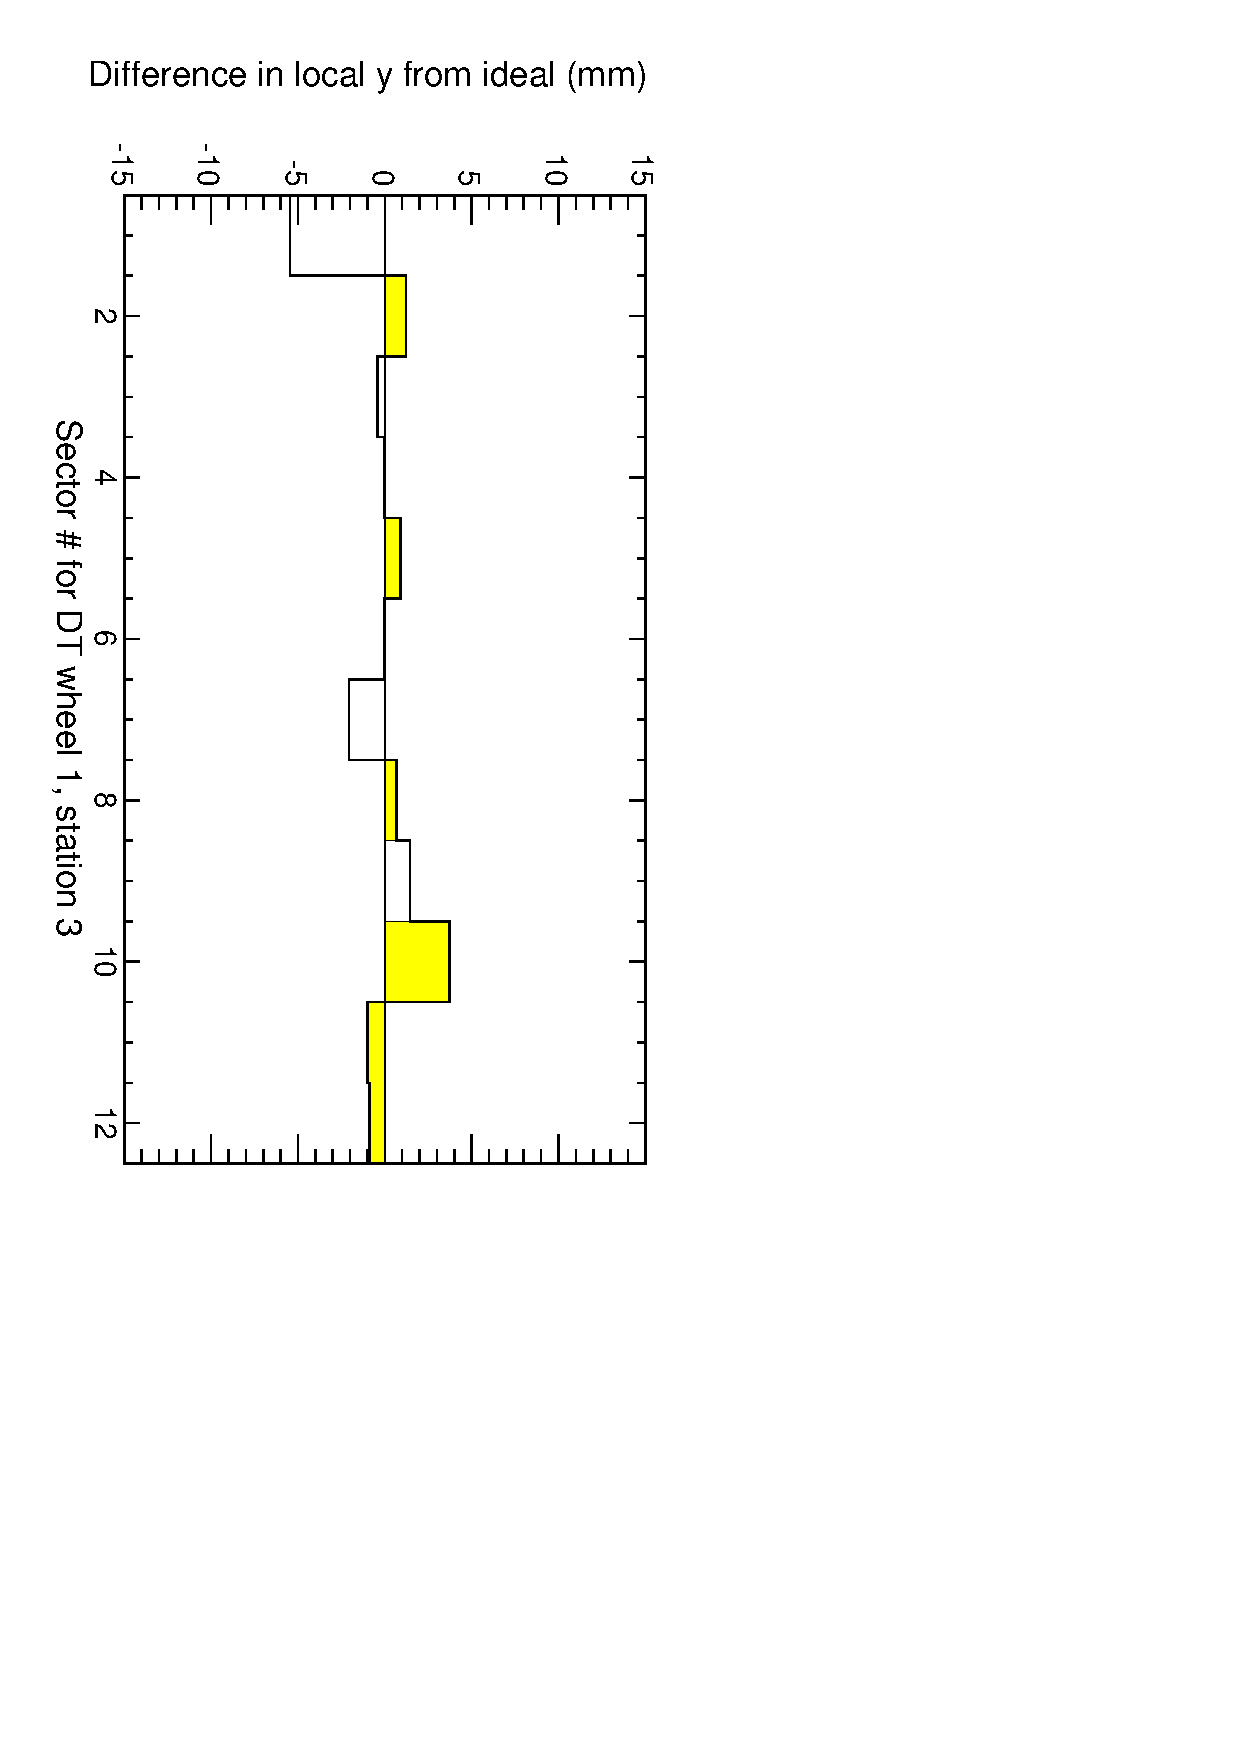
\includegraphics[height=0.5\linewidth, angle=90]{DThist033.pdf} \\
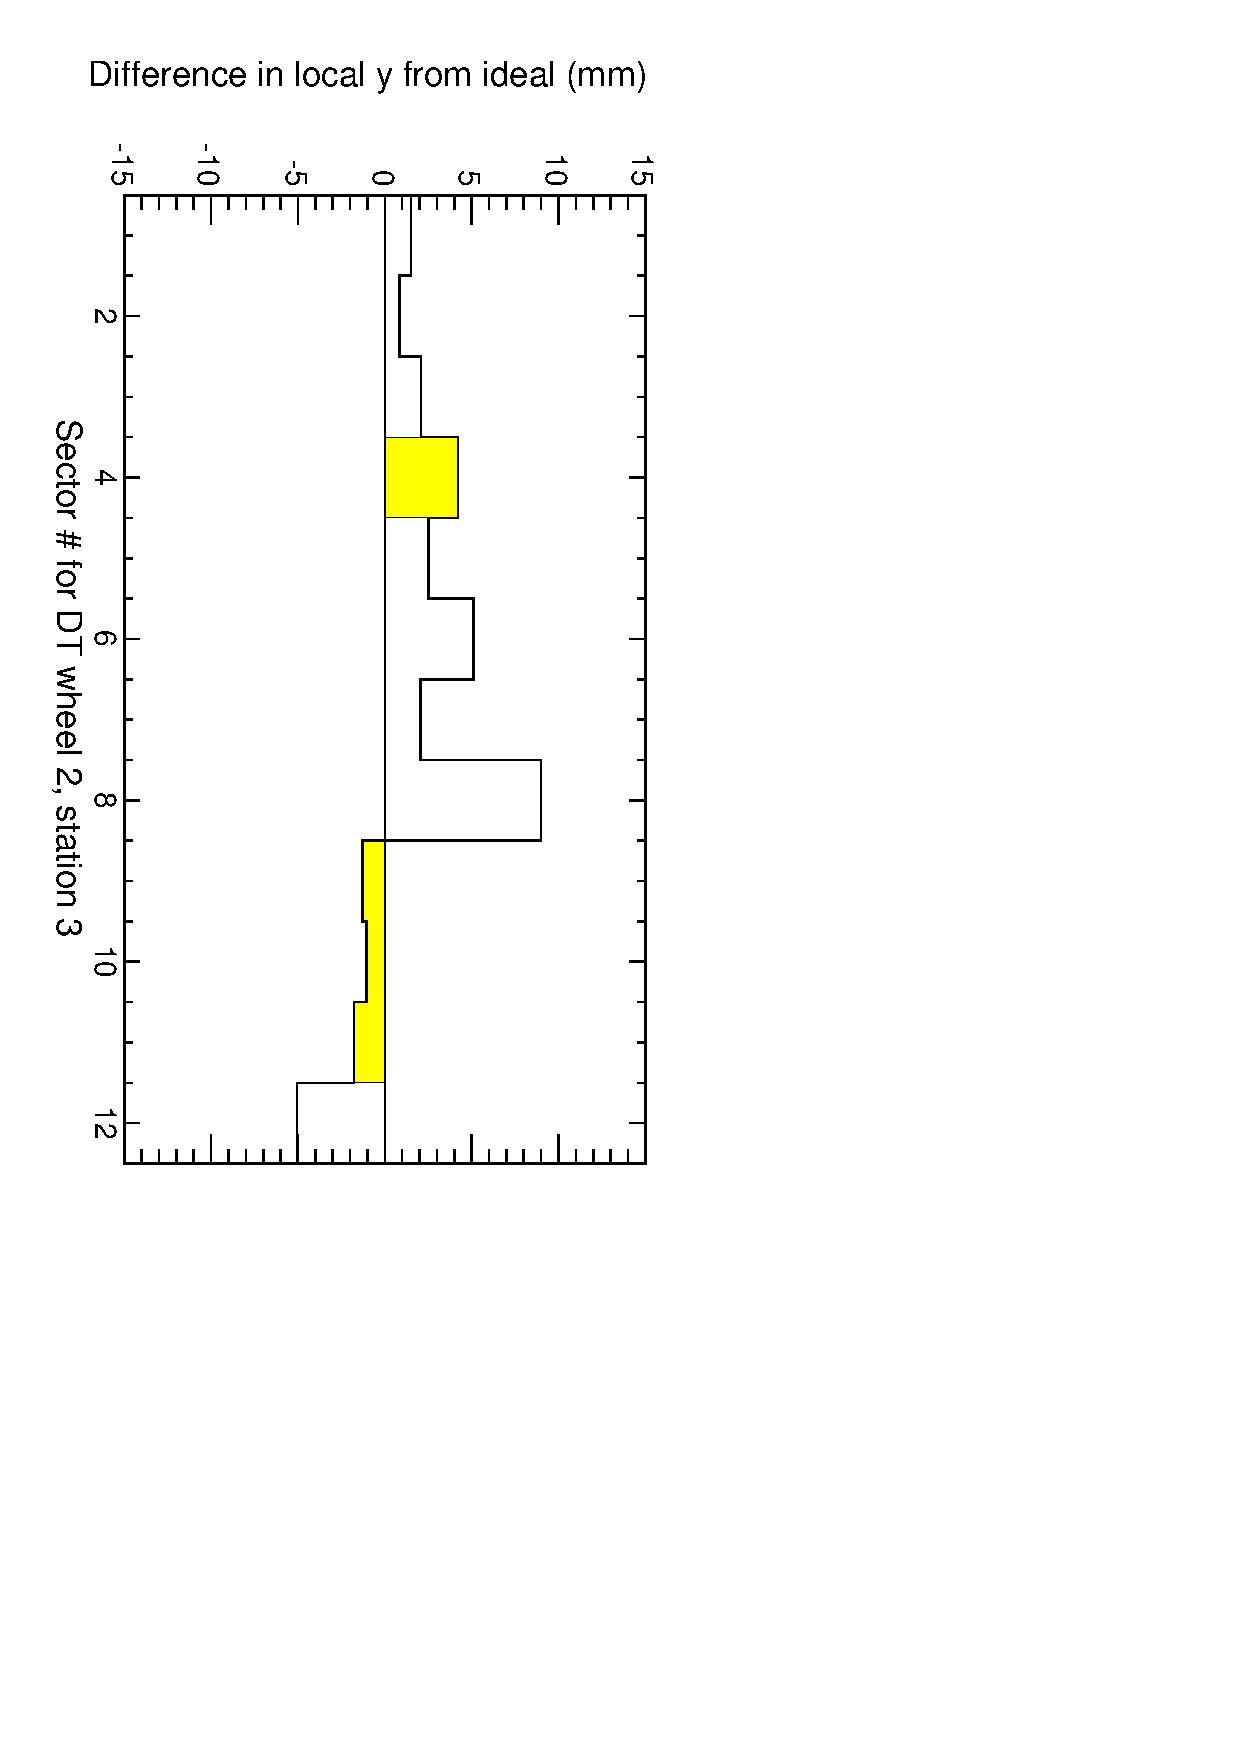
\includegraphics[height=0.5\linewidth, angle=90]{DThist034.pdf} 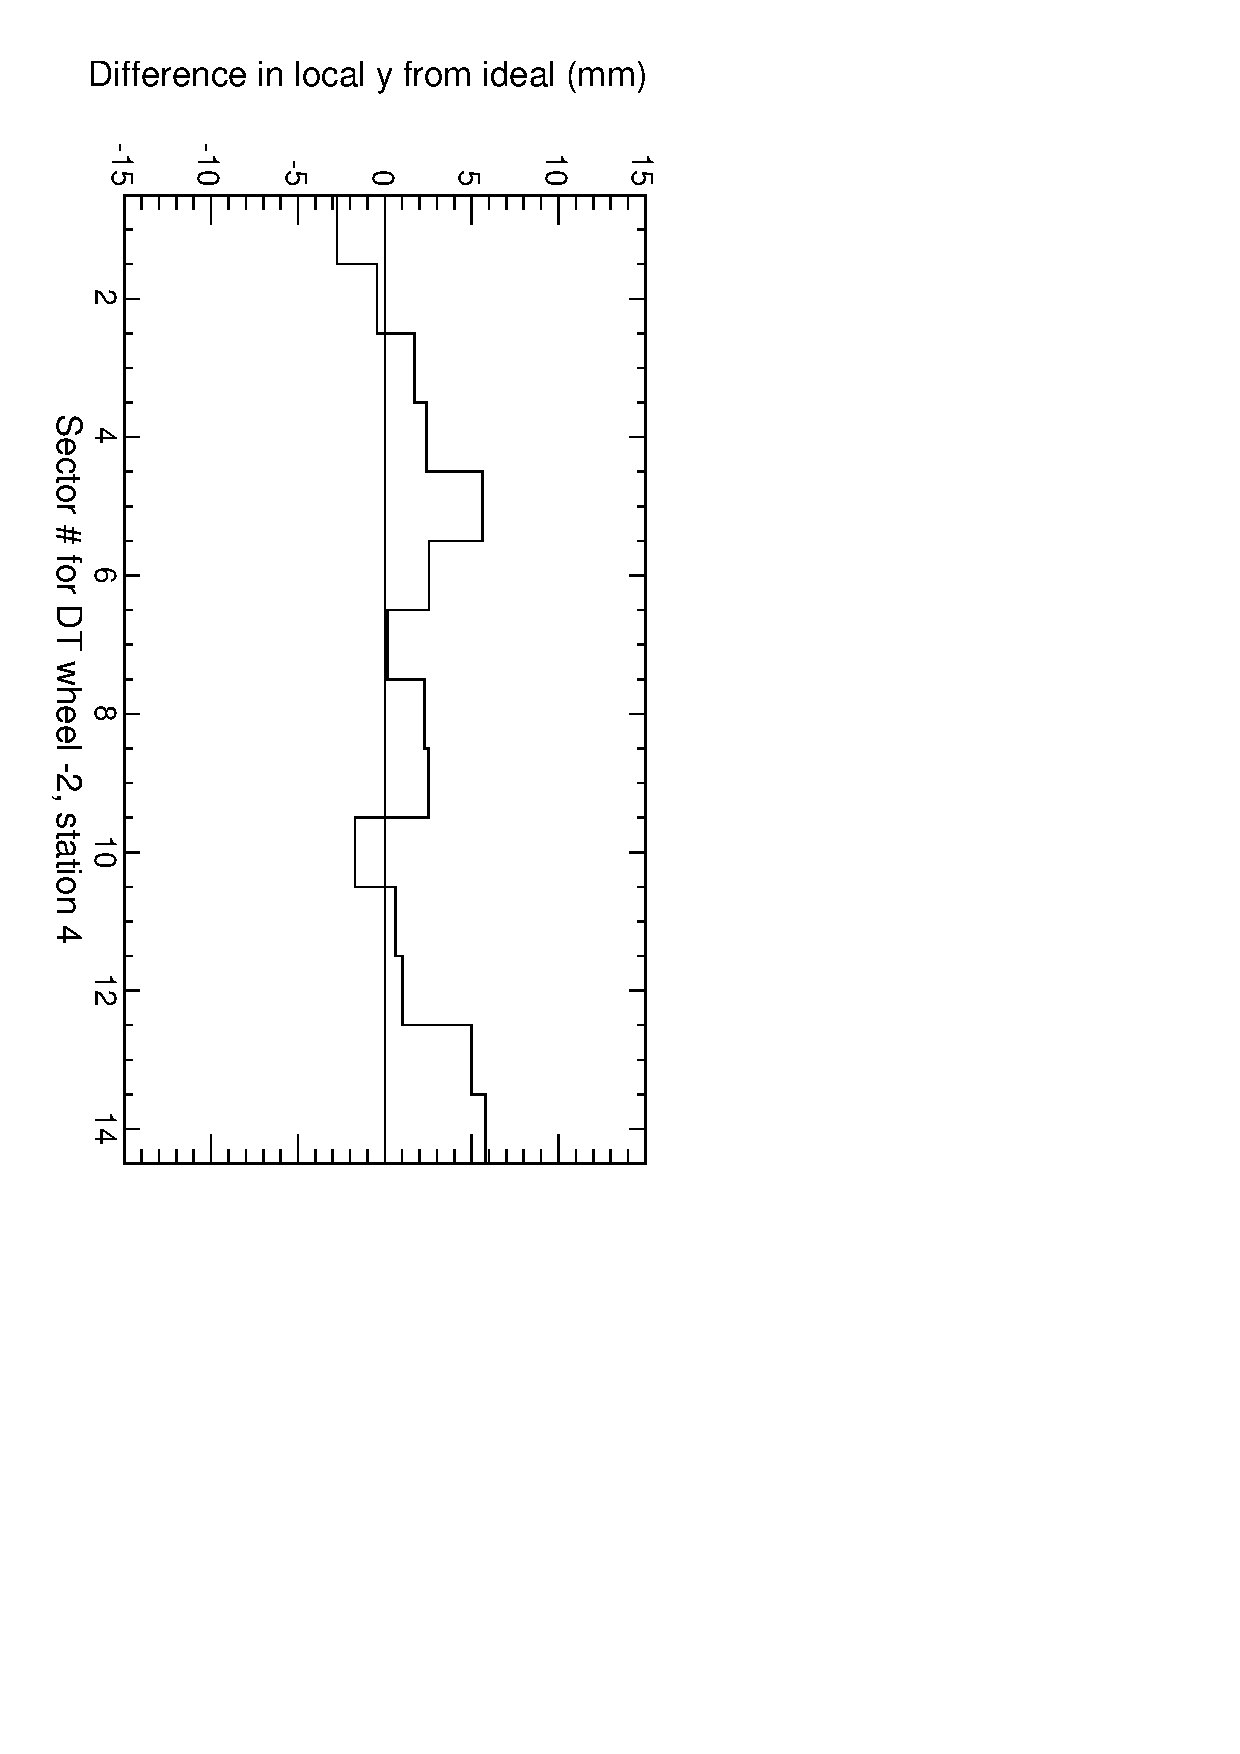
\includegraphics[height=0.5\linewidth, angle=90]{DThist035.pdf}
\end{frame}

\begin{frame}
\frametitle{Reference: all the constants}
\framesubtitle{Yellow denotes a parameter that was aligned with globalMuons}
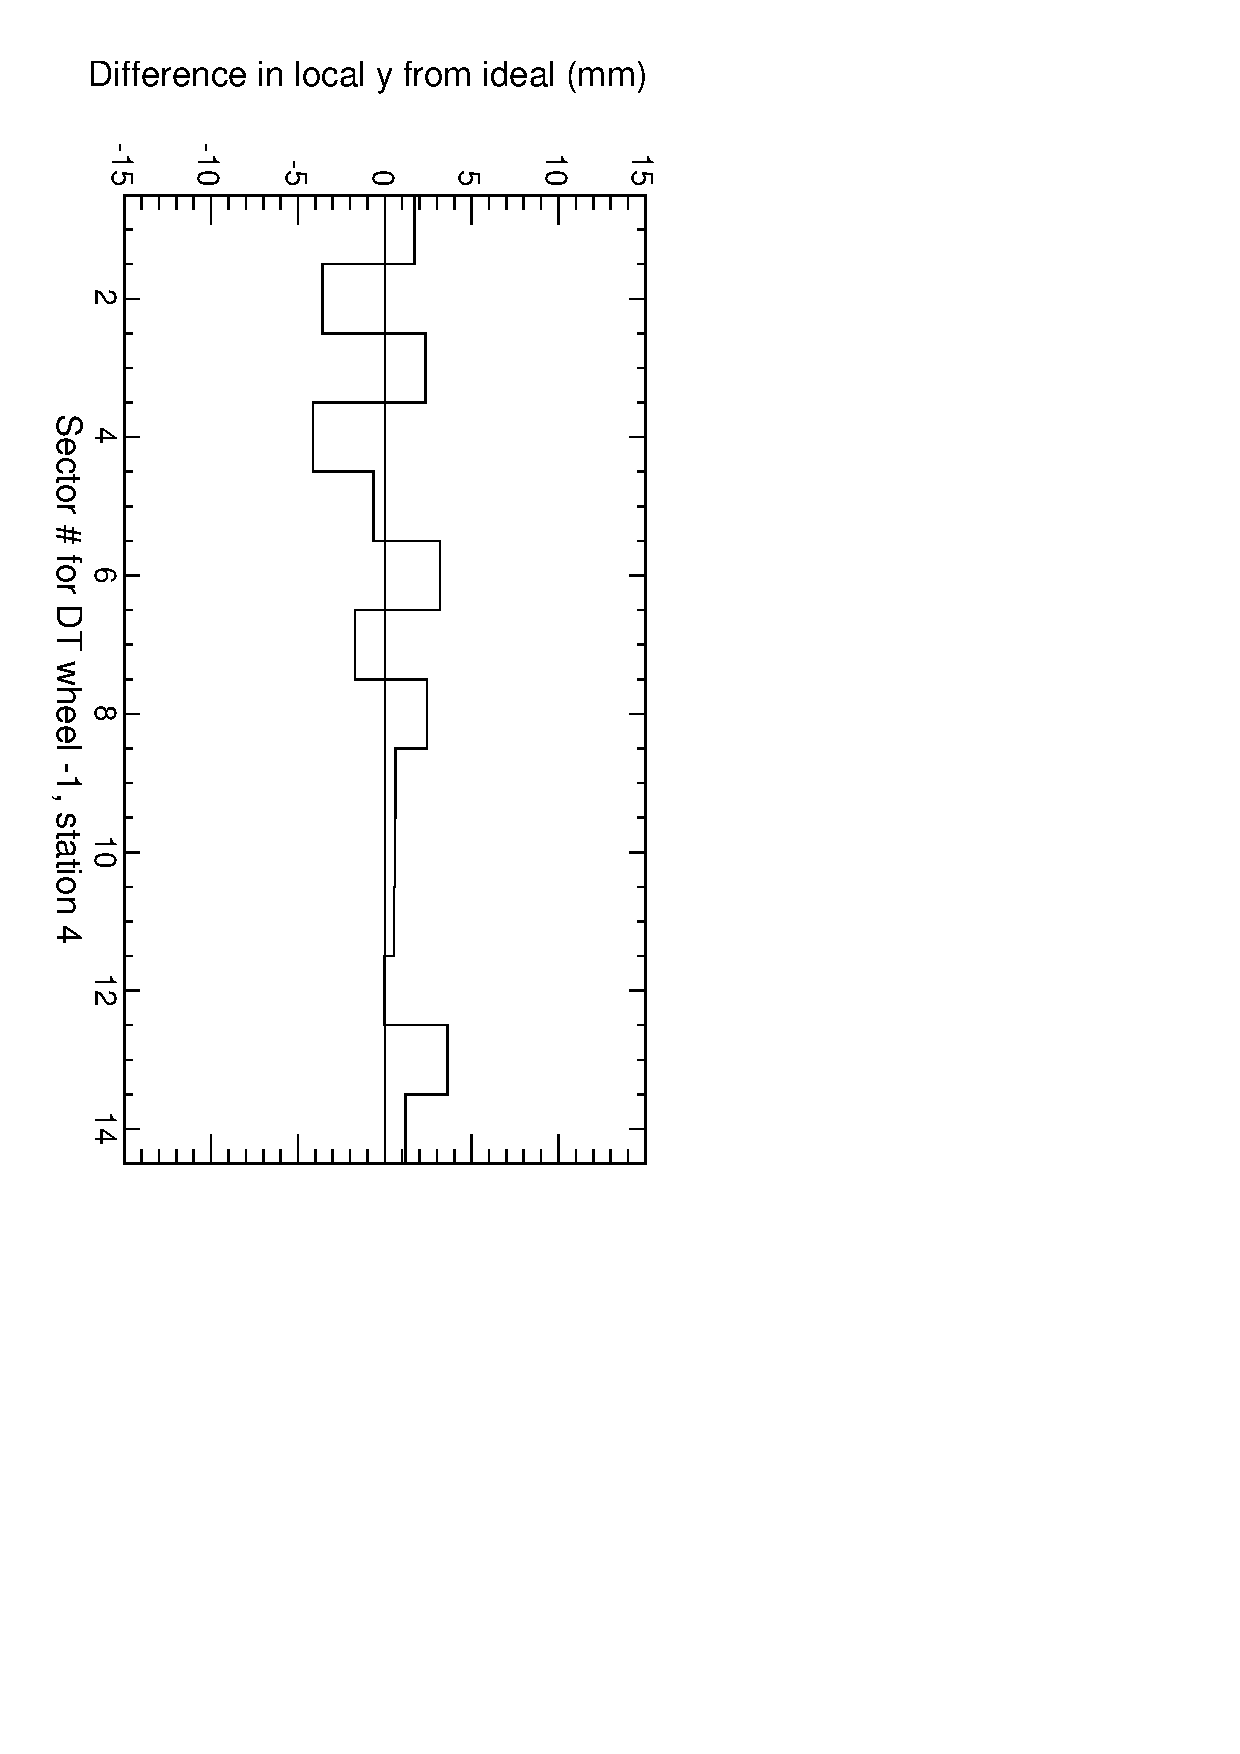
\includegraphics[height=0.5\linewidth, angle=90]{DThist036.pdf} 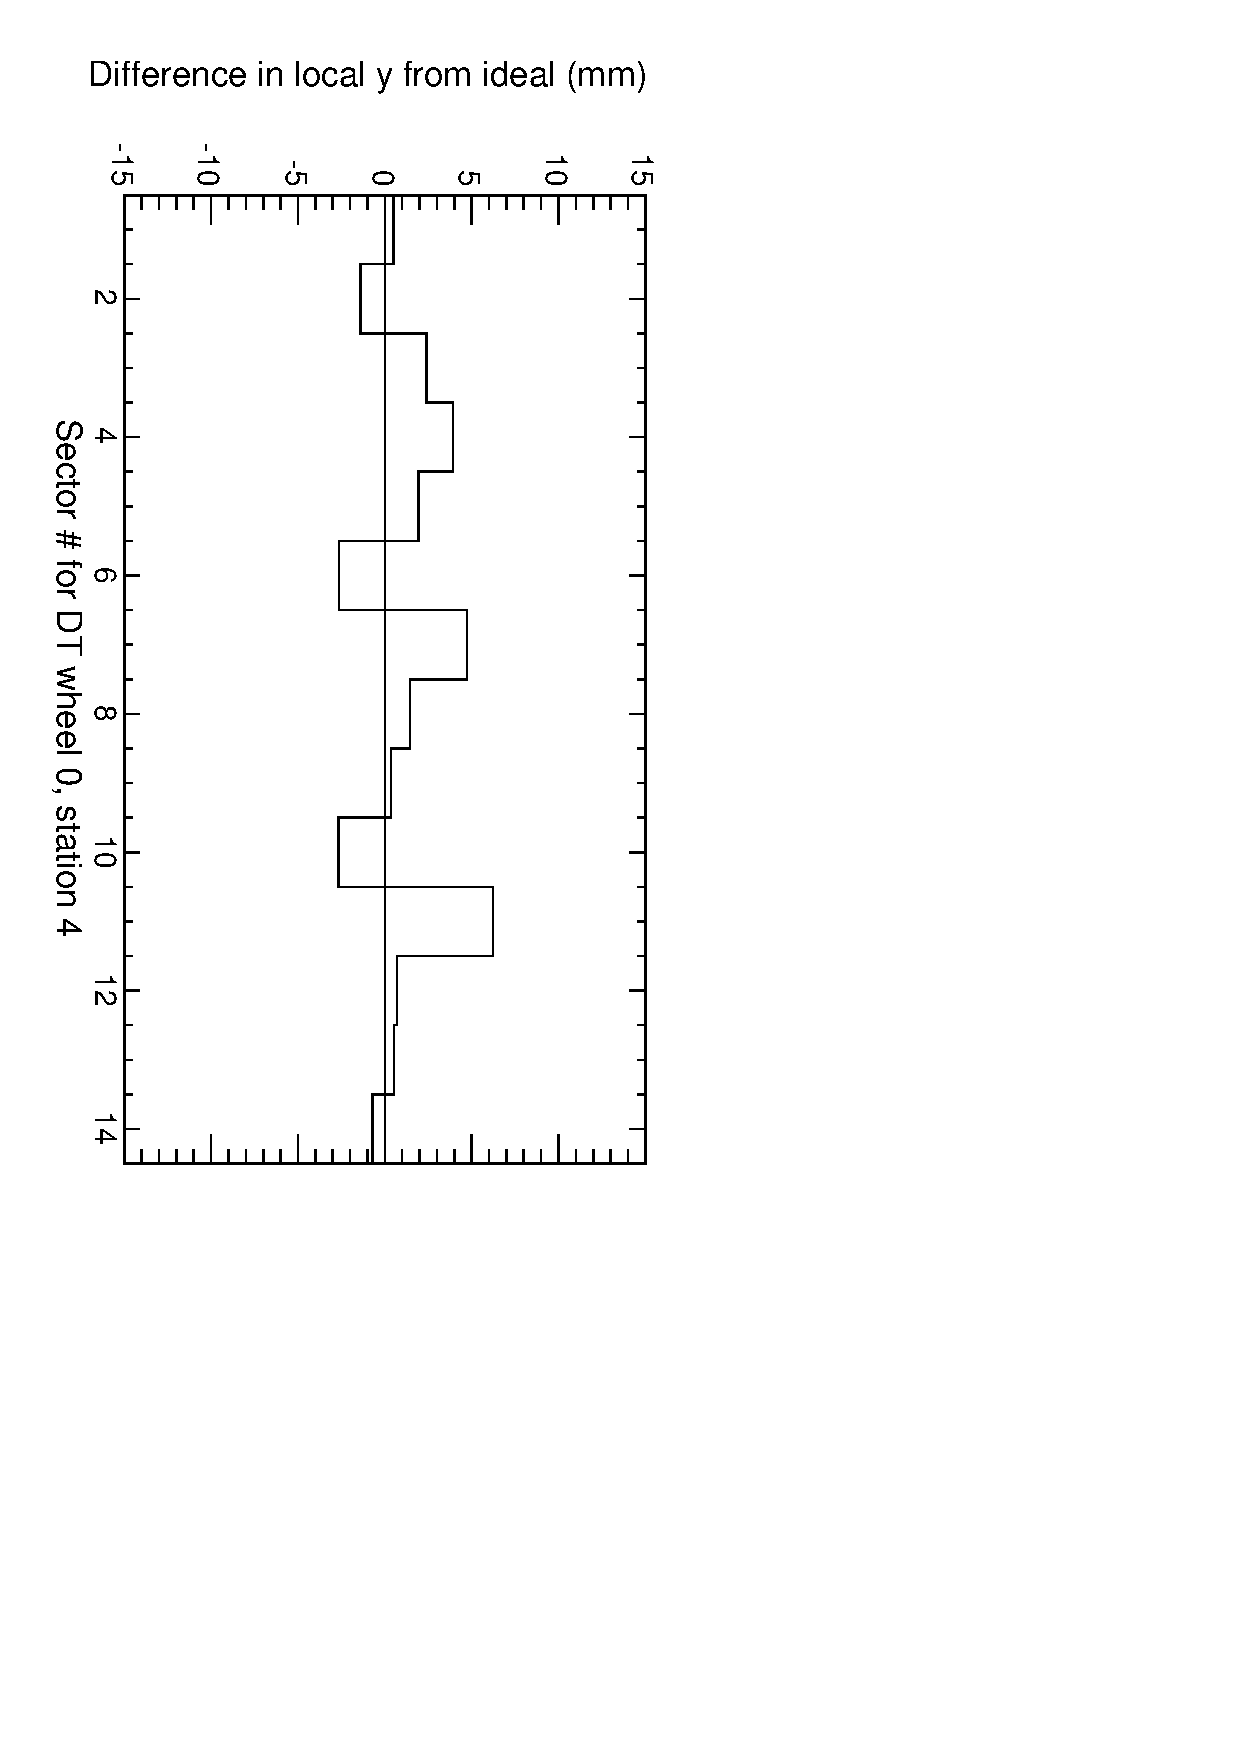
\includegraphics[height=0.5\linewidth, angle=90]{DThist037.pdf} \\
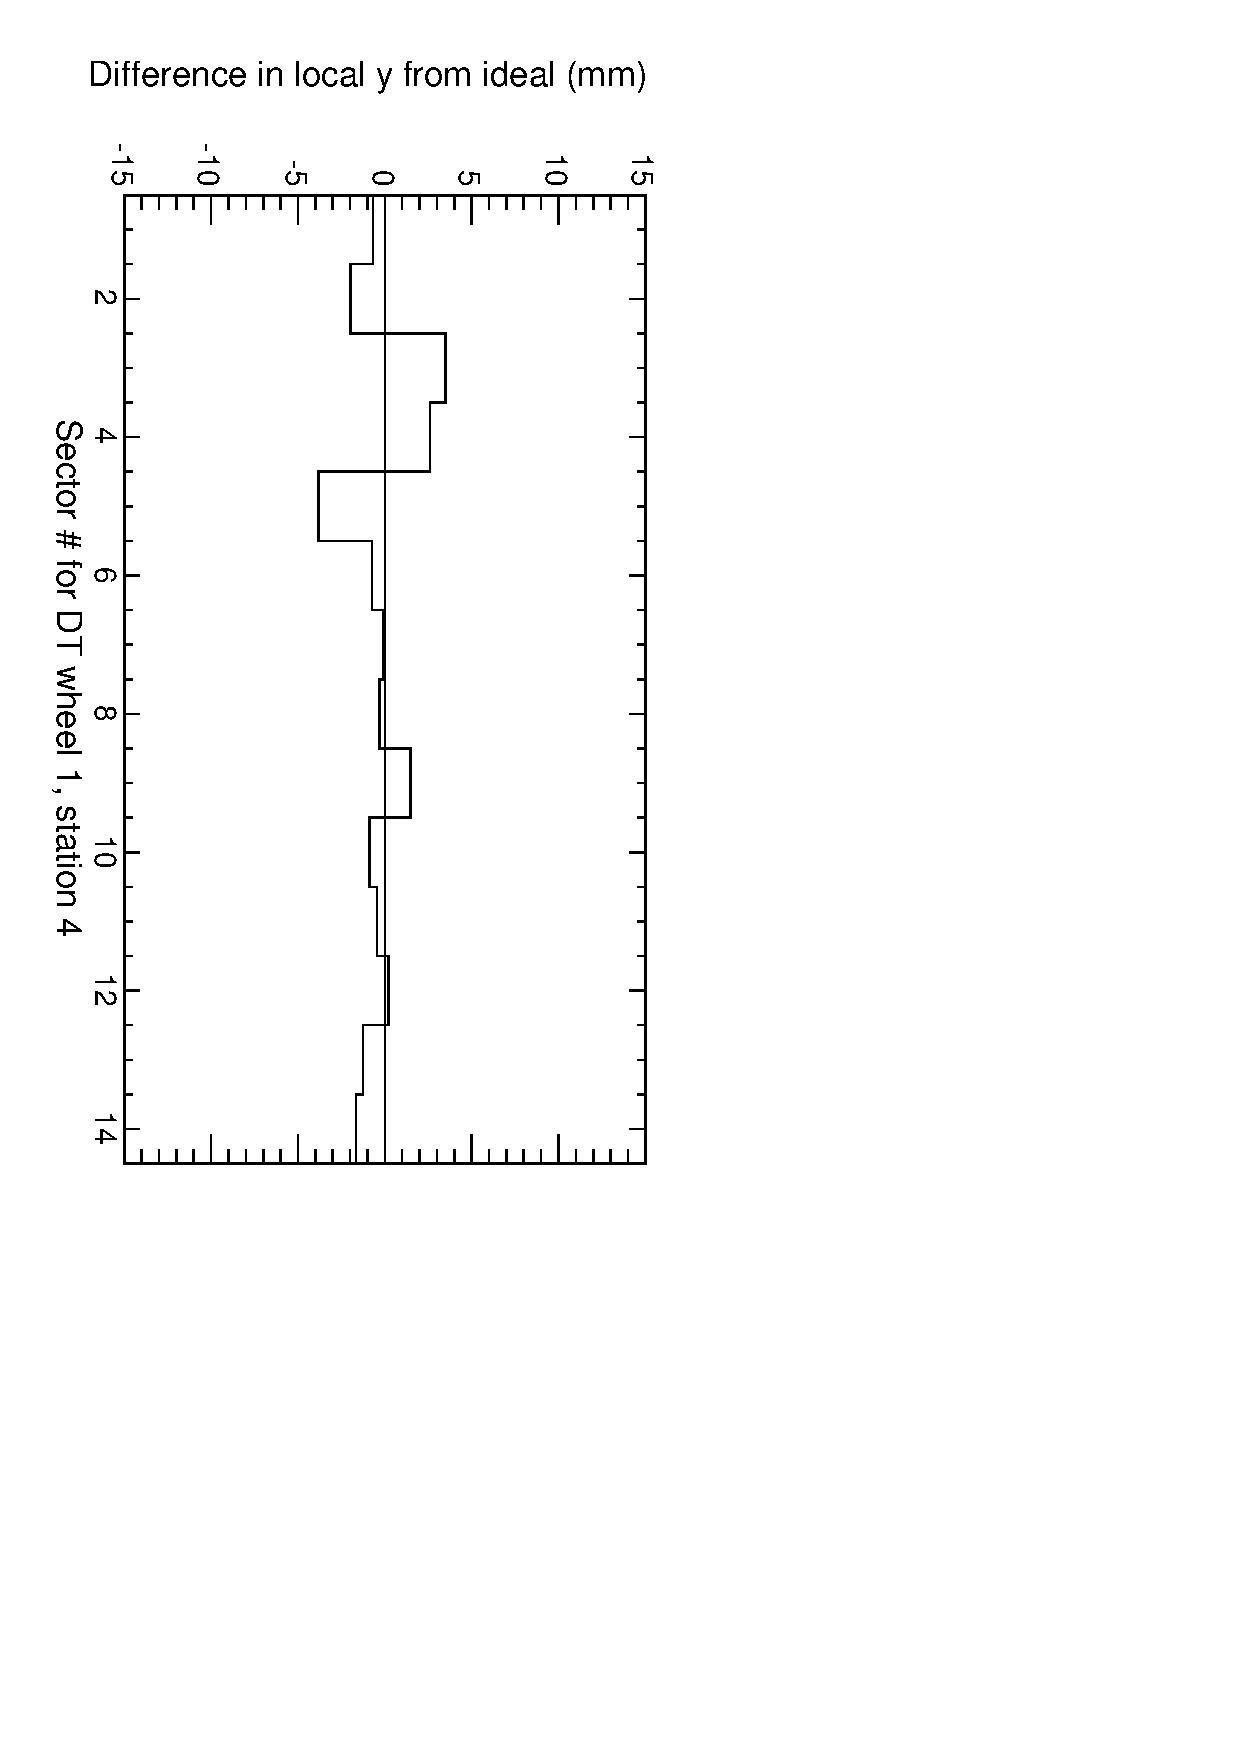
\includegraphics[height=0.5\linewidth, angle=90]{DThist038.pdf} 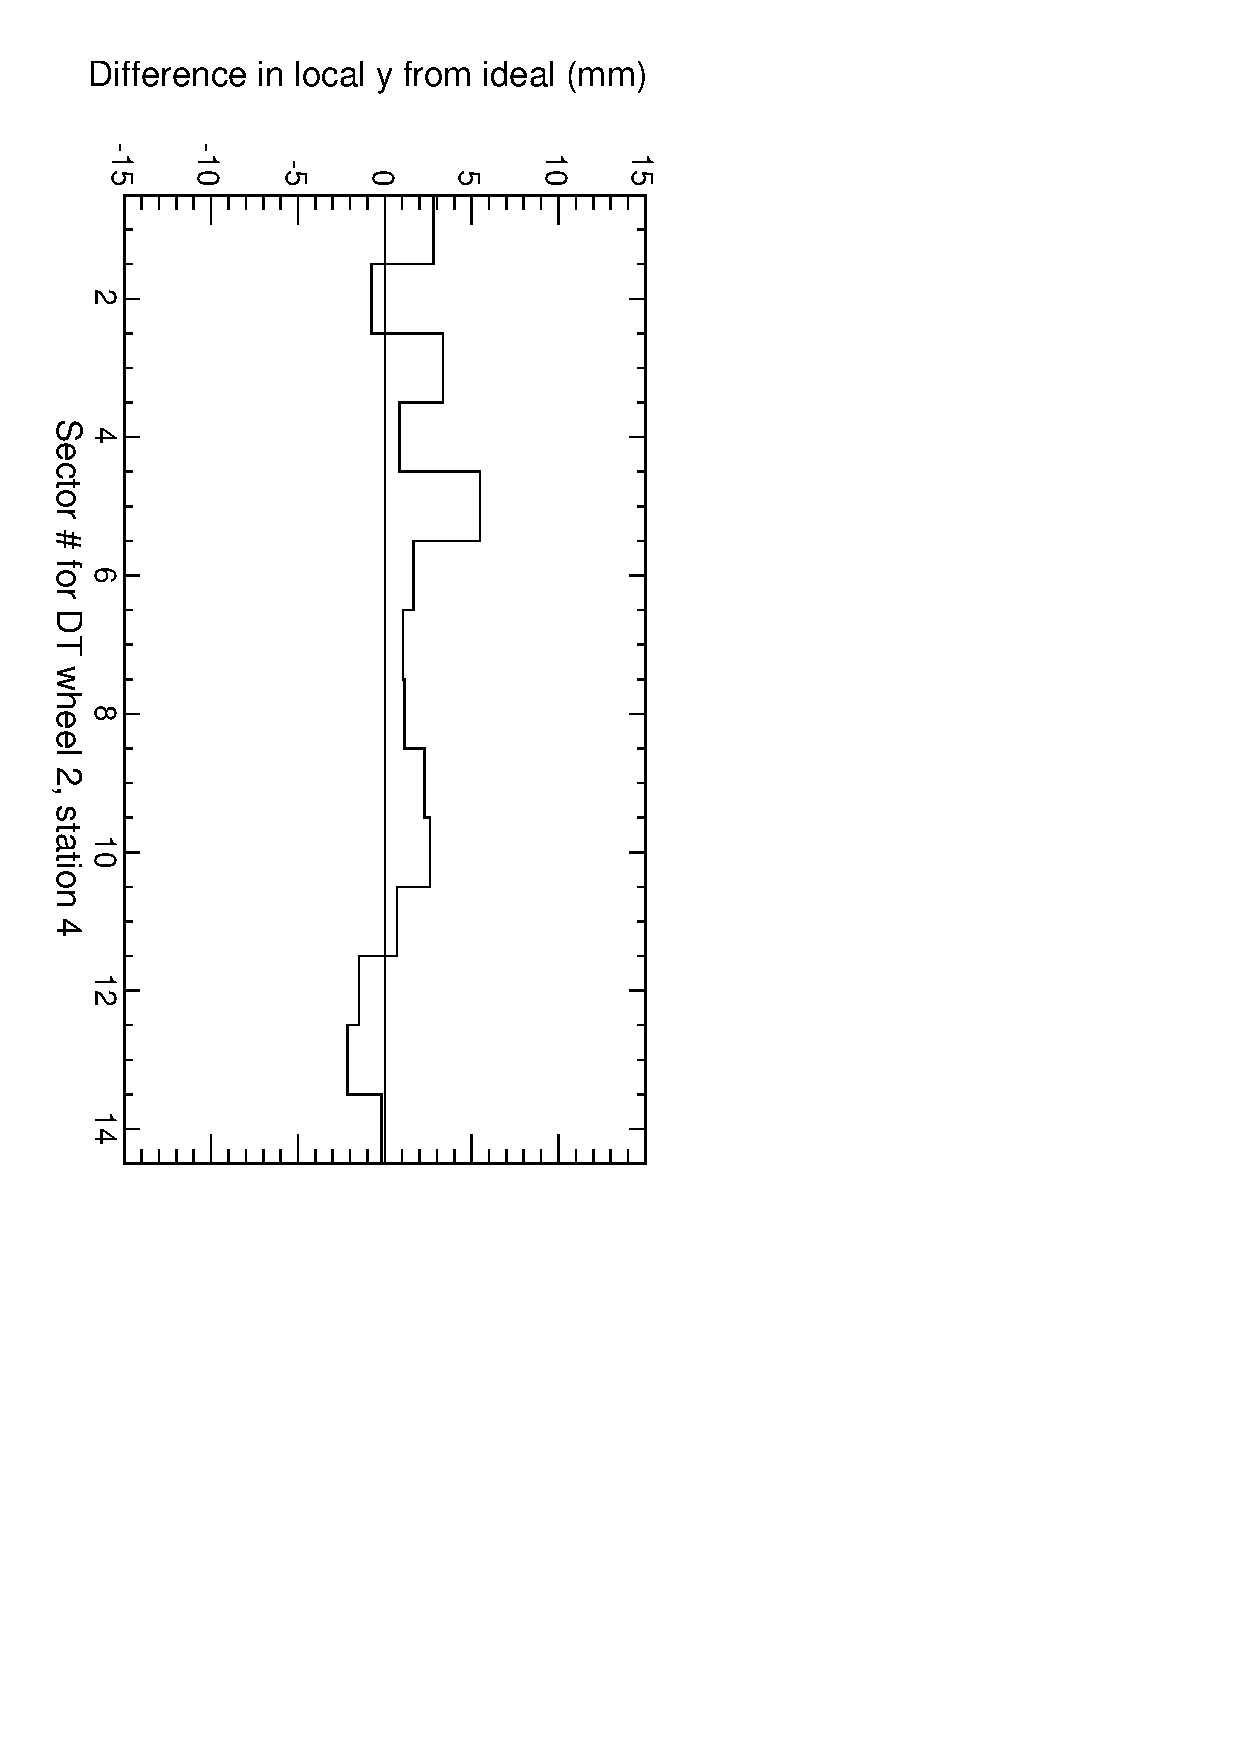
\includegraphics[height=0.5\linewidth, angle=90]{DThist039.pdf}
\end{frame}

\begin{frame}
\frametitle{Reference: all the constants}
\framesubtitle{Yellow denotes a parameter that was aligned with globalMuons}
\includegraphics[height=0.5\linewidth, angle=90]{DThist040.pdf} \includegraphics[height=0.5\linewidth, angle=90]{DThist041.pdf} \\
\includegraphics[height=0.5\linewidth, angle=90]{DThist042.pdf} \includegraphics[height=0.5\linewidth, angle=90]{DThist043.pdf}
\end{frame}

\begin{frame}
\frametitle{Reference: all the constants}
\framesubtitle{Yellow denotes a parameter that was aligned with globalMuons}
\includegraphics[height=0.5\linewidth, angle=90]{DThist044.pdf} \includegraphics[height=0.5\linewidth, angle=90]{DThist045.pdf} \\
\includegraphics[height=0.5\linewidth, angle=90]{DThist046.pdf} \includegraphics[height=0.5\linewidth, angle=90]{DThist047.pdf}
\end{frame}

\begin{frame}
\frametitle{Reference: all the constants}
\framesubtitle{Yellow denotes a parameter that was aligned with globalMuons}
\includegraphics[height=0.5\linewidth, angle=90]{DThist048.pdf} \includegraphics[height=0.5\linewidth, angle=90]{DThist049.pdf} \\
\includegraphics[height=0.5\linewidth, angle=90]{DThist050.pdf} \includegraphics[height=0.5\linewidth, angle=90]{DThist051.pdf}
\end{frame}

\begin{frame}
\frametitle{Reference: all the constants}
\framesubtitle{Yellow denotes a parameter that was aligned with globalMuons}
\includegraphics[height=0.5\linewidth, angle=90]{DThist052.pdf} \includegraphics[height=0.5\linewidth, angle=90]{DThist053.pdf} \\
\includegraphics[height=0.5\linewidth, angle=90]{DThist054.pdf} \includegraphics[height=0.5\linewidth, angle=90]{DThist055.pdf}
\end{frame}

\begin{frame}
\frametitle{Reference: all the constants}
\framesubtitle{Yellow denotes a parameter that was aligned with globalMuons}
\includegraphics[height=0.5\linewidth, angle=90]{DThist056.pdf} \includegraphics[height=0.5\linewidth, angle=90]{DThist057.pdf} \\
\includegraphics[height=0.5\linewidth, angle=90]{DThist058.pdf} \includegraphics[height=0.5\linewidth, angle=90]{DThist059.pdf}
\end{frame}

\begin{frame}
\frametitle{Reference: all the constants}
\framesubtitle{Yellow denotes a parameter that was aligned with globalMuons}
\includegraphics[height=0.5\linewidth, angle=90]{DThist060.pdf} \includegraphics[height=0.5\linewidth, angle=90]{DThist061.pdf} \\
\includegraphics[height=0.5\linewidth, angle=90]{DThist062.pdf} \includegraphics[height=0.5\linewidth, angle=90]{DThist063.pdf}
\end{frame}

\begin{frame}
\frametitle{Reference: all the constants}
\framesubtitle{Yellow denotes a parameter that was aligned with globalMuons}
\includegraphics[height=0.5\linewidth, angle=90]{DThist064.pdf} \includegraphics[height=0.5\linewidth, angle=90]{DThist065.pdf} \\
\includegraphics[height=0.5\linewidth, angle=90]{DThist066.pdf} \includegraphics[height=0.5\linewidth, angle=90]{DThist067.pdf}
\end{frame}

\begin{frame}
\frametitle{Reference: all the constants}
\framesubtitle{Yellow denotes a parameter that was aligned with globalMuons}
\includegraphics[height=0.5\linewidth, angle=90]{DThist068.pdf} \includegraphics[height=0.5\linewidth, angle=90]{DThist069.pdf} \\
\includegraphics[height=0.5\linewidth, angle=90]{DThist070.pdf} \includegraphics[height=0.5\linewidth, angle=90]{DThist071.pdf}
\end{frame}

\begin{frame}
\frametitle{Reference: all the constants}
\framesubtitle{Yellow denotes a parameter that was aligned with globalMuons}
\includegraphics[height=0.5\linewidth, angle=90]{DThist072.pdf} \includegraphics[height=0.5\linewidth, angle=90]{DThist073.pdf} \\
\includegraphics[height=0.5\linewidth, angle=90]{DThist074.pdf} \includegraphics[height=0.5\linewidth, angle=90]{DThist075.pdf}
\end{frame}

\begin{frame}
\frametitle{Reference: all the constants}
\framesubtitle{Yellow denotes a parameter that was aligned with globalMuons}
\includegraphics[height=0.5\linewidth, angle=90]{DThist076.pdf} \includegraphics[height=0.5\linewidth, angle=90]{DThist077.pdf} \\
\includegraphics[height=0.5\linewidth, angle=90]{DThist078.pdf} \includegraphics[height=0.5\linewidth, angle=90]{DThist079.pdf}
\end{frame}

\begin{frame}
\frametitle{Reference: all the constants}
\framesubtitle{Yellow denotes a parameter that was aligned with globalMuons}
\includegraphics[height=0.5\linewidth, angle=90]{DThist080.pdf} \includegraphics[height=0.5\linewidth, angle=90]{DThist081.pdf} \\
\includegraphics[height=0.5\linewidth, angle=90]{DThist082.pdf} \includegraphics[height=0.5\linewidth, angle=90]{DThist083.pdf}
\end{frame}

\begin{frame}
\frametitle{Reference: all the constants}
\framesubtitle{Yellow denotes a parameter that was aligned with globalMuons}
\includegraphics[height=0.5\linewidth, angle=90]{DThist084.pdf} \includegraphics[height=0.5\linewidth, angle=90]{DThist085.pdf} \\
\includegraphics[height=0.5\linewidth, angle=90]{DThist086.pdf} \includegraphics[height=0.5\linewidth, angle=90]{DThist087.pdf}
\end{frame}

\begin{frame}
\frametitle{Reference: all the constants}
\framesubtitle{Yellow denotes a parameter that was aligned with globalMuons}
\includegraphics[height=0.5\linewidth, angle=90]{DThist088.pdf} \includegraphics[height=0.5\linewidth, angle=90]{DThist089.pdf} \\
\includegraphics[height=0.5\linewidth, angle=90]{DThist090.pdf} \includegraphics[height=0.5\linewidth, angle=90]{DThist091.pdf}
\end{frame}

\begin{frame}
\frametitle{Reference: all the constants}
\framesubtitle{Yellow denotes a parameter that was aligned with globalMuons}
\includegraphics[height=0.5\linewidth, angle=90]{DThist092.pdf} \includegraphics[height=0.5\linewidth, angle=90]{DThist093.pdf} \\
\includegraphics[height=0.5\linewidth, angle=90]{DThist094.pdf} \includegraphics[height=0.5\linewidth, angle=90]{DThist095.pdf}
\end{frame}

\begin{frame}
\frametitle{Reference: all the constants}
\framesubtitle{Yellow denotes a parameter that was aligned with globalMuons}
\includegraphics[height=0.5\linewidth, angle=90]{DThist096.pdf} \includegraphics[height=0.5\linewidth, angle=90]{DThist097.pdf} \\
\includegraphics[height=0.5\linewidth, angle=90]{DThist098.pdf} \includegraphics[height=0.5\linewidth, angle=90]{DThist099.pdf}
\end{frame}

\begin{frame}
\frametitle{Reference: all the constants}
\framesubtitle{Yellow denotes a parameter that was aligned with globalMuons}
\includegraphics[height=0.5\linewidth, angle=90]{DThist100.pdf} \includegraphics[height=0.5\linewidth, angle=90]{DThist101.pdf} \\
\includegraphics[height=0.5\linewidth, angle=90]{DThist102.pdf} \includegraphics[height=0.5\linewidth, angle=90]{DThist103.pdf}
\end{frame}

\begin{frame}
\frametitle{Reference: all the constants}
\framesubtitle{Yellow denotes a parameter that was aligned with globalMuons}
\includegraphics[height=0.5\linewidth, angle=90]{DThist104.pdf} \includegraphics[height=0.5\linewidth, angle=90]{DThist105.pdf} \\
\includegraphics[height=0.5\linewidth, angle=90]{DThist106.pdf} \includegraphics[height=0.5\linewidth, angle=90]{DThist107.pdf}
\end{frame}

\begin{frame}
\frametitle{Reference: all the constants}
\framesubtitle{Yellow denotes a parameter that was aligned with globalMuons}
\includegraphics[height=0.5\linewidth, angle=90]{DThist108.pdf} \includegraphics[height=0.5\linewidth, angle=90]{DThist109.pdf} \\
\includegraphics[height=0.5\linewidth, angle=90]{DThist110.pdf} \includegraphics[height=0.5\linewidth, angle=90]{DThist111.pdf}
\end{frame}

\begin{frame}
\frametitle{Reference: all the constants}
\framesubtitle{Yellow denotes a parameter that was aligned with globalMuons}
\includegraphics[height=0.5\linewidth, angle=90]{DThist112.pdf} \includegraphics[height=0.5\linewidth, angle=90]{DThist113.pdf} \\
\includegraphics[height=0.5\linewidth, angle=90]{DThist114.pdf} \includegraphics[height=0.5\linewidth, angle=90]{DThist115.pdf}
\end{frame}

\begin{frame}
\frametitle{Reference: all the constants}
\framesubtitle{Yellow denotes a parameter that was aligned with globalMuons}
\includegraphics[height=0.5\linewidth, angle=90]{DThist116.pdf} \includegraphics[height=0.5\linewidth, angle=90]{DThist117.pdf} \\
\includegraphics[height=0.5\linewidth, angle=90]{DThist118.pdf} \includegraphics[height=0.5\linewidth, angle=90]{DThist119.pdf}
\end{frame}

\begin{frame}
\frametitle{Reference: all the constants}
\framesubtitle{Yellow denotes a parameter that was aligned with globalMuons}
\includegraphics[height=0.5\linewidth, angle=90]{CSChist000.pdf} \includegraphics[height=0.5\linewidth, angle=90]{CSChist001.pdf} \\
\includegraphics[height=0.5\linewidth, angle=90]{CSChist002.pdf} \includegraphics[height=0.5\linewidth, angle=90]{CSChist003.pdf}
\end{frame}

\begin{frame}
\frametitle{Reference: all the constants}
\framesubtitle{Yellow denotes a parameter that was aligned with globalMuons}
\includegraphics[height=0.5\linewidth, angle=90]{CSChist004.pdf} \includegraphics[height=0.5\linewidth, angle=90]{CSChist005.pdf} \\
\includegraphics[height=0.5\linewidth, angle=90]{CSChist006.pdf} \includegraphics[height=0.5\linewidth, angle=90]{CSChist007.pdf}
\end{frame}

\begin{frame}
\frametitle{Reference: all the constants}
\framesubtitle{Yellow denotes a parameter that was aligned with globalMuons}
\includegraphics[height=0.5\linewidth, angle=90]{CSChist008.pdf} \includegraphics[height=0.5\linewidth, angle=90]{CSChist009.pdf} \\
\includegraphics[height=0.5\linewidth, angle=90]{CSChist010.pdf} \includegraphics[height=0.5\linewidth, angle=90]{CSChist011.pdf}
\end{frame}

\begin{frame}
\frametitle{Reference: all the constants}
\framesubtitle{Yellow denotes a parameter that was aligned with globalMuons}
\includegraphics[height=0.5\linewidth, angle=90]{CSChist012.pdf} \includegraphics[height=0.5\linewidth, angle=90]{CSChist013.pdf} \\
\includegraphics[height=0.5\linewidth, angle=90]{CSChist014.pdf} \includegraphics[height=0.5\linewidth, angle=90]{CSChist015.pdf}
\end{frame}

\begin{frame}
\frametitle{Reference: all the constants}
\framesubtitle{Yellow denotes a parameter that was aligned with globalMuons}
\includegraphics[height=0.5\linewidth, angle=90]{CSChist016.pdf} \includegraphics[height=0.5\linewidth, angle=90]{CSChist017.pdf} \\
\includegraphics[height=0.5\linewidth, angle=90]{CSChist018.pdf} \includegraphics[height=0.5\linewidth, angle=90]{CSChist019.pdf}
\end{frame}

\begin{frame}
\frametitle{Reference: all the constants}
\framesubtitle{Yellow denotes a parameter that was aligned with globalMuons}
\includegraphics[height=0.5\linewidth, angle=90]{CSChist020.pdf} \includegraphics[height=0.5\linewidth, angle=90]{CSChist021.pdf} \\
\includegraphics[height=0.5\linewidth, angle=90]{CSChist022.pdf} \includegraphics[height=0.5\linewidth, angle=90]{CSChist023.pdf}
\end{frame}

\begin{frame}
\frametitle{Reference: all the constants}
\framesubtitle{Yellow denotes a parameter that was aligned with globalMuons}
\includegraphics[height=0.5\linewidth, angle=90]{CSChist024.pdf} \includegraphics[height=0.5\linewidth, angle=90]{CSChist025.pdf} \\
\includegraphics[height=0.5\linewidth, angle=90]{CSChist026.pdf} \includegraphics[height=0.5\linewidth, angle=90]{CSChist027.pdf}
\end{frame}

\begin{frame}
\frametitle{Reference: all the constants}
\framesubtitle{Yellow denotes a parameter that was aligned with globalMuons}
\includegraphics[height=0.5\linewidth, angle=90]{CSChist028.pdf} \includegraphics[height=0.5\linewidth, angle=90]{CSChist029.pdf} \\
\includegraphics[height=0.5\linewidth, angle=90]{CSChist030.pdf} \includegraphics[height=0.5\linewidth, angle=90]{CSChist031.pdf}
\end{frame}

\begin{frame}
\frametitle{Reference: all the constants}
\framesubtitle{Yellow denotes a parameter that was aligned with globalMuons}
\includegraphics[height=0.5\linewidth, angle=90]{CSChist032.pdf} \includegraphics[height=0.5\linewidth, angle=90]{CSChist033.pdf} \\
\includegraphics[height=0.5\linewidth, angle=90]{CSChist034.pdf} \includegraphics[height=0.5\linewidth, angle=90]{CSChist035.pdf}
\end{frame}

\begin{frame}
\frametitle{Reference: all the constants}
\framesubtitle{Yellow denotes a parameter that was aligned with globalMuons}
\includegraphics[height=0.5\linewidth, angle=90]{CSChist036.pdf} \includegraphics[height=0.5\linewidth, angle=90]{CSChist037.pdf} \\
\includegraphics[height=0.5\linewidth, angle=90]{CSChist038.pdf} \includegraphics[height=0.5\linewidth, angle=90]{CSChist039.pdf}
\end{frame}

\begin{frame}
\frametitle{Reference: all the constants}
\framesubtitle{Yellow denotes a parameter that was aligned with globalMuons}
\includegraphics[height=0.5\linewidth, angle=90]{CSChist040.pdf} \includegraphics[height=0.5\linewidth, angle=90]{CSChist041.pdf} \\
\includegraphics[height=0.5\linewidth, angle=90]{CSChist042.pdf} \includegraphics[height=0.5\linewidth, angle=90]{CSChist043.pdf}
\end{frame}

\begin{frame}
\frametitle{Reference: all the constants}
\framesubtitle{Yellow denotes a parameter that was aligned with globalMuons}
\includegraphics[height=0.5\linewidth, angle=90]{CSChist044.pdf} \includegraphics[height=0.5\linewidth, angle=90]{CSChist045.pdf} \\
\includegraphics[height=0.5\linewidth, angle=90]{CSChist046.pdf} \includegraphics[height=0.5\linewidth, angle=90]{CSChist047.pdf}
\end{frame}

\begin{frame}
\frametitle{Reference: all the constants}
\framesubtitle{Yellow denotes a parameter that was aligned with globalMuons}
\includegraphics[height=0.5\linewidth, angle=90]{CSChist048.pdf} \includegraphics[height=0.5\linewidth, angle=90]{CSChist049.pdf} \\
\includegraphics[height=0.5\linewidth, angle=90]{CSChist050.pdf} \includegraphics[height=0.5\linewidth, angle=90]{CSChist051.pdf}
\end{frame}

\begin{frame}
\frametitle{Reference: all the constants}
\framesubtitle{Yellow denotes a parameter that was aligned with globalMuons}
\includegraphics[height=0.5\linewidth, angle=90]{CSChist052.pdf} \includegraphics[height=0.5\linewidth, angle=90]{CSChist053.pdf} \\
\includegraphics[height=0.5\linewidth, angle=90]{CSChist054.pdf} \includegraphics[height=0.5\linewidth, angle=90]{CSChist055.pdf}
\end{frame}

\begin{frame}
\frametitle{Reference: all the constants}
\framesubtitle{Yellow denotes a parameter that was aligned with globalMuons}
\includegraphics[height=0.5\linewidth, angle=90]{CSChist056.pdf} \includegraphics[height=0.5\linewidth, angle=90]{CSChist057.pdf} \\
\includegraphics[height=0.5\linewidth, angle=90]{CSChist058.pdf} \includegraphics[height=0.5\linewidth, angle=90]{CSChist059.pdf}
\end{frame}

\begin{frame}
\frametitle{Reference: all the constants}
\framesubtitle{Yellow denotes a parameter that was aligned with globalMuons}
\includegraphics[height=0.5\linewidth, angle=90]{CSChist060.pdf} \includegraphics[height=0.5\linewidth, angle=90]{CSChist061.pdf} \\
\includegraphics[height=0.5\linewidth, angle=90]{CSChist062.pdf} \includegraphics[height=0.5\linewidth, angle=90]{CSChist063.pdf}
\end{frame}

\begin{frame}
\frametitle{Reference: all the constants}
\framesubtitle{Yellow denotes a parameter that was aligned with globalMuons}
\includegraphics[height=0.5\linewidth, angle=90]{CSChist064.pdf} \includegraphics[height=0.5\linewidth, angle=90]{CSChist065.pdf} \\
\includegraphics[height=0.5\linewidth, angle=90]{CSChist066.pdf} \includegraphics[height=0.5\linewidth, angle=90]{CSChist067.pdf}
\end{frame}

\begin{frame}
\frametitle{Reference: all the constants}
\framesubtitle{Yellow denotes a parameter that was aligned with globalMuons}
\includegraphics[height=0.5\linewidth, angle=90]{CSChist068.pdf} \includegraphics[height=0.5\linewidth, angle=90]{CSChist069.pdf} \\
\includegraphics[height=0.5\linewidth, angle=90]{CSChist070.pdf} \includegraphics[height=0.5\linewidth, angle=90]{CSChist071.pdf}
\end{frame}

\begin{frame}
\frametitle{Reference: all the constants}
\framesubtitle{Yellow denotes a parameter that was aligned with globalMuons}
\includegraphics[height=0.5\linewidth, angle=90]{CSChist072.pdf} \includegraphics[height=0.5\linewidth, angle=90]{CSChist073.pdf} \\
\includegraphics[height=0.5\linewidth, angle=90]{CSChist074.pdf} \includegraphics[height=0.5\linewidth, angle=90]{CSChist075.pdf}
\end{frame}

\begin{frame}
\frametitle{Reference: all the constants}
\framesubtitle{Yellow denotes a parameter that was aligned with globalMuons}
\includegraphics[height=0.5\linewidth, angle=90]{CSChist076.pdf} \includegraphics[height=0.5\linewidth, angle=90]{CSChist077.pdf} \\
\includegraphics[height=0.5\linewidth, angle=90]{CSChist078.pdf} \includegraphics[height=0.5\linewidth, angle=90]{CSChist079.pdf}
\end{frame}

\begin{frame}
\frametitle{Reference: all the constants}
\framesubtitle{Yellow denotes a parameter that was aligned with globalMuons}
\includegraphics[height=0.5\linewidth, angle=90]{CSChist080.pdf} \includegraphics[height=0.5\linewidth, angle=90]{CSChist081.pdf} \\
\includegraphics[height=0.5\linewidth, angle=90]{CSChist082.pdf} \includegraphics[height=0.5\linewidth, angle=90]{CSChist083.pdf}
\end{frame}

\begin{frame}
\frametitle{Reference: all the constants}
\framesubtitle{Yellow denotes a parameter that was aligned with globalMuons}
\includegraphics[height=0.5\linewidth, angle=90]{CSChist084.pdf} \includegraphics[height=0.5\linewidth, angle=90]{CSChist085.pdf} \\
\includegraphics[height=0.5\linewidth, angle=90]{CSChist086.pdf} \includegraphics[height=0.5\linewidth, angle=90]{CSChist087.pdf}
\end{frame}

\begin{frame}
\frametitle{Reference: all the constants}
\framesubtitle{Yellow denotes a parameter that was aligned with globalMuons}
\includegraphics[height=0.5\linewidth, angle=90]{CSChist088.pdf} \includegraphics[height=0.5\linewidth, angle=90]{CSChist089.pdf} \\
\includegraphics[height=0.5\linewidth, angle=90]{CSChist090.pdf} \includegraphics[height=0.5\linewidth, angle=90]{CSChist091.pdf}
\end{frame}

\begin{frame}
\frametitle{Reference: all the constants}
\framesubtitle{Yellow denotes a parameter that was aligned with globalMuons}
\includegraphics[height=0.5\linewidth, angle=90]{CSChist092.pdf} \includegraphics[height=0.5\linewidth, angle=90]{CSChist093.pdf} \\
\includegraphics[height=0.5\linewidth, angle=90]{CSChist094.pdf} \includegraphics[height=0.5\linewidth, angle=90]{CSChist095.pdf}
\end{frame}

\begin{frame}
\frametitle{Reference: all the constants}
\framesubtitle{Yellow denotes a parameter that was aligned with globalMuons}
\includegraphics[height=0.5\linewidth, angle=90]{CSChist096.pdf} \includegraphics[height=0.5\linewidth, angle=90]{CSChist097.pdf} \\
\includegraphics[height=0.5\linewidth, angle=90]{CSChist098.pdf} \includegraphics[height=0.5\linewidth, angle=90]{CSChist099.pdf}
\end{frame}

\begin{frame}
\frametitle{Reference: all the constants}
\framesubtitle{Yellow denotes a parameter that was aligned with globalMuons}
\includegraphics[height=0.5\linewidth, angle=90]{CSChist100.pdf} \includegraphics[height=0.5\linewidth, angle=90]{CSChist101.pdf} \\
\includegraphics[height=0.5\linewidth, angle=90]{CSChist102.pdf} \includegraphics[height=0.5\linewidth, angle=90]{CSChist103.pdf}
\end{frame}

\begin{frame}
\frametitle{Reference: all the constants}
\framesubtitle{Yellow denotes a parameter that was aligned with globalMuons}
\includegraphics[height=0.5\linewidth, angle=90]{CSChist104.pdf} \includegraphics[height=0.5\linewidth, angle=90]{CSChist105.pdf} \\
\includegraphics[height=0.5\linewidth, angle=90]{CSChist106.pdf} \includegraphics[height=0.5\linewidth, angle=90]{CSChist107.pdf}
\end{frame}

\end{document}
